%%%%%%%%%%%%%%%%%%%%%%%%%%%%%%%%%%%%%%%%%%%%%%%%%%%%%%%
%                 File: OSAtemp.tex                   %
%                Date: Sept. 2. 2009                  %
%                                                     %
%    LaTeX template file for use with OSA journals    %
%         JOSA A, JOSA B, and Applied Optics          %
%
%                                                     %
%   This file requires the substyle file osajnl2.rtx, %
%       running under REVTeX 4.0 and LaTeX 2e,        %
%                           or                        %
%   the style file osajnl2.sty, running under LaTeX 2e%
%                                                     %
%       USE THE FOLLOWING REVTEX 4.0 OPTIONS:         %
%  \documentclass[osajnl2,preprint,showpacs]{revtex4} %
%                                                     %
%         USE THE FOLLOWING LaTeX OPTIONS:            %
%           \documentclass[12pt]{article}             %
%           \usepackage{osajnl2}                      %
%                                                     %
%                                                     %
%      (C) 2009 The Optical Society of America        %
%                                                     %
%%%%%%%%%%%%%%%%%%%%%%%%%%%%%%%%%%%%%%%%%%%%%%%%%%%%%%%

%\documentclass[12pt,osajnl2,preprint,showpacs]{revtex4}  %% REVTeX 4.0

%%%%%%%%%%%%%%%%%%%%%%%%%%%%%%%%%%%%%%%%%%%%%%%%%%%%%%%%%%%%%%%%
%% Delete any REVTEX output files before running in LaTeX mode
%%%%%%%%%%%%%%%%%%%%%%%%%%%%%%%%%%%%%%%%%%%%%%%%%%%%%%%%%%%%%%%%%

\documentclass[letterpaper,12pt]{article}   %% LaTeX 2e (preferred)
\usepackage{osajnl2} %% do not use with REVTeX4
\usepackage[draft,implicit=false]{hyperref} %% optional
\usepackage{caption}
\usepackage{subcaption}
\usepackage{algcompatible}
\usepackage{algorithm}
%\usepackage{algorithmic}
\usepackage{chngpage}
\usepackage{geometry}
\usepackage{wrapfig}
\usepackage{amsfonts}
%This then gives you access to:
%\begin{wrapfigure}[lineheight]{position}{width}

%****************************************************************************
% Shireen Elhabian formating additions

\newenvironment{myindentpar}[1]%
     {\begin{list}{}%
             {\setlength{\leftmargin}{#1}\setlength{\rightmargin}{#1}}%
             \item[]%
     }
     {\end{list}}
     

\setlength{\parskip}{0pt}
\setlength{\parsep}{0pt}
\setlength{\headsep}{0pt}
\setlength{\topskip}{0pt}
\setlength{\topmargin}{0pt}
\setlength{\topsep}{0pt}
\setlength{\partopsep}{0pt}
\setlength{\itemsep}{0pt}
\setlength{\textfloatsep}{0.1in}%{-0.2in}
\setlength{\intextsep}{0pt}
\setlength{\dblfloatsep}{0.05in}
\setlength{\dbltextfloatsep}{0.1in}
\setlength{\belowcaptionskip}{0in}
\setlength{\abovecaptionskip}{0in}
%\setlength{\bibsep}{0.0pt}
\setlength{\belowdisplayskip}{0pt} \setlength{\belowdisplayshortskip}{0pt}
\setlength{\abovedisplayskip}{0pt} \setlength{\abovedisplayshortskip}{0pt}


%****************************************************************************
\usepackage{amsmath}
\usepackage{listings}
%\newcommand{\argmin}{\operatornamewithlimits{argmin}}
%\newcommand{\argmax}{\operatornamewithlimits{argmax}}

\DeclareMathOperator*{\argmax}{arg\!\max}

%% to have figures at the top of the page
%\makeatletter
%\setlength{\@fptop}{0pt}
%\makeatother

\lstdefinestyle{BashInputStyle}{
  language=bash,
  basicstyle=\small\ttfamily,
  %numbers=left,
  numberstyle=\tiny,
  numbersep=3pt,
  %frame=tb,
  framerule=1pt,
  %columns=fullflexible
  frame=single,
  breaklines=true,
  postbreak=\raisebox{0ex}[0ex][0ex]{\ensuremath{\color{red}\hookrightarrow\space}}
}

\usepackage{wrapfig}
\graphicspath{{figures/}}
\begin{document}

\title{ShapeWorksStudio v2.2 \\ Particle-based Shape Correspondence and Visualization Software}
\begin{figure}
\centering
%
\includegraphics[scale=1]{figs/shapes-icon.png}

\includegraphics[scale=0.9]{figs_v2/studio.png}\vspace{0.05in}
\end{figure}

%% For REVTeX it is possible to automate superscript and e-mail callouts with the superscriptaddress option; see REVTeX4 documentation.


%\author{ShapeWorks Team}
\author{Shireen Elhabian, Praful Agrawal, Joshua Cates, Manasi Datar, Ross Whitaker}
\vspace{0.05in}
\email{shapeworks-users@sci.utah.edu}
\vspace{0.2in}
\address{Scientific Computing and Imaging Institute, School of Computing, \\University of Utah, Salt Lake City, UT 84112, USA}

\vspace{0.2in}

\hrule
\vspace{0.1in}
\noindent Shapeworks\footnote{\texttt{https://www.sci.utah.edu/software/shapeworks.html}} and the associated user-friendly graphical interface ShapeworksStudio\footnote{\texttt{https://github.com/SCIInstitute/ShapeworksStudio/releases}} are open-source distributions of a new method for
constructing compact statistical point-based models of ensembles of similar shapes that does not rely on any specific surface parameterization. It is developed by the NIH Center for Integrative Biomedical Computing at the University of Utah Scientific Computing and Imaging (SCI) Institute.
\vspace{0.1in}
\hrule

\tableofcontents
%\vspace{0.02in}
\hrule
\newpage

\section{License}

ShapeWorks and its graphical user interface ShapeWorksStudio are available for free and are open source under the MIT License. For more information, please refer to \texttt{https://www.sci.utah.edu/software/shapeworks.html}.

The MIT License Copyright (c) 2012 Scientific Computing and Imaging Institute, University of Utah. License for the specific language governing rights and limitations under Permission is hereby granted, free of charge, to any person obtaining a copy of this software and associated documentation files (the "Software"), to deal in the Software without restriction, including without limitation the rights to use, copy, modify, merge, publish, distribute, sublicense, and/or sell copies of the Software, and to permit persons to whom the Software is furnished to do so, subject to the following conditions: The above copyright notice and this permission notice shall be included in all copies or substantial portions of the Software. THE SOFTWARE IS PROVIDED "AS IS", WITHOUT WARRANTY OF ANY KIND, EXPRESS OR IMPLIED, INCLUDING BUT NOT LIMITED TO THE WARRANTIES OF MERCHANTABILITY, FITNESS FOR A PARTICULAR PURPOSE AND NONINFRINGEMENT. IN NO EVENT SHALL THE AUTHORS OR COPYRIGHT HOLDERS BE LIABLE FOR ANY CLAIM, DAMAGES OR OTHER LIABILITY, WHETHER IN AN ACTION OF CONTRACT, TORT OR OTHERWISE, ARISING FROM, OUT OF OR IN CONNECTION WITH THE SOFTWARE OR THE USE OR OTHER DEALINGS IN THE SOFTWARE.

\section{Acknowledgement}

If you use ShapeWorks and/or ShapeWorksStudio in work that leads to published research, we humbly ask that you add the following to the 'Acknowledgments' section of your paper: \textit{"This project was supported by the National Institute of General Medical Sciences of the National Institutes of Health under grant number P41 GM103545-18."}

\section{Introduction}

This software is an open source distribution of the algorithm for constructing correspondence-based statistical models of sets of similar shapes, originally created and maintained by the research group of Dr. Whitaker at the University of Utah \cite{cates2006entropy,cates2007shape,cates2008particle,oguz2015entropy,cates2017shapeworks}.  The scientific and clinical effectiveness of ShapeWorks and its underlying scientific premise of particle-based shape modeling have been demonstrated in a range of applications, including neuroscience \cite{cates2008particle,oguz2008cortical,oguz2009cortical,datar2009particle,datar2013geodesic,sultana2016towards},
biological phenotyping \cite{cates2008shape,jones2013toward}, orthopedics \cite{jones2013toward,harris2013statistical,atkins2016quantitative}, and cardiology \cite{cates2015computational,gardner2013point}. This document is intended to provide necessary background information for understanding and using the ShapeWorksStudio software, including a basic tutorial and reference. This section gives a technical overview of correspondence shape models and the correspondence optimization algorithm that is implemented in the ShapeWorks software. For a more detailed explanation of the ShapeWorks optimization algorithm, please refer to \cite{cates2007shape,cates2017shapeworks}.

\subsection{Particle-based correspondence models} 


\textit{Manually defined landmarks} have been the most popular choice for a light-weight, general shape representation that is suitable for statistical analysis and visual communication of the results \cite{sarkalkan2014statistical,zachow2015computational}. ShapeWorks provides an important paradigm shift from manually defined anatomical homologies to computationally derived {\em correspondence shape models} that are constructed automatically from 3D images of anatomy (i.e., computed tomography (CT) and magnetic resonance imaging (MRI)). Without relying on any surface parameterization, ShapeWorks enables a generalized and flexible approach to handling general anatomy with arbitrary topology compared to existing tools for surface-based analysis that are either tailored to specific anatomical structures or restrict modeling to spherical topologies. In particular, ShapeWorks computes a statistically optimal representation of the population variability by choosing landmark positions that minimize the overall information content of the model while maintaining a good sampling of surface geometry. 

Correspondence point models represent shape by sampling each shape surface in a consistently ordered fashion so as to define homologous surface points across the population of shapes. These homologous surface points are called \textit{correspondences}. Once chosen, the 3D positions of all $m$ correspondences on a shape sample can be encoded as a $3m$ shape vector, which is the point-based representation of that shape. The ordering of the particles on each shape implies a correspondence among shapes, and the distribution of all of the shape samples in this $3m$-dimensional vector space (\textit{shape space}) gives rise to the statistical analysis. The problem of how to choose the correspondence positions, and thus the shape-space distribution of the sample population, is a model selection problem. Model selection problems in statistics are typically resolved by choosing the simplest model that explains the observed data (see, e.g., \cite{hansen2001model}). Consistent with this idea, the ShapeWorks correspondence optimization algorithm seeks a compact distribution for its correspondences in the shape space (for model simplicity), while simultaneously seeking good surface samplings in order to accurately represent the data. Fig \ref{fig:overview} illustrates these basic concepts for a population of hand shapes. The figure shows the mapping of all the surface point samples from a single shape to a single point in the higher- dimensional shape space, and the relative compactness of the distribution of all samples in that shape space after optimization.


\begin{figure}[!htp]
	\centering
	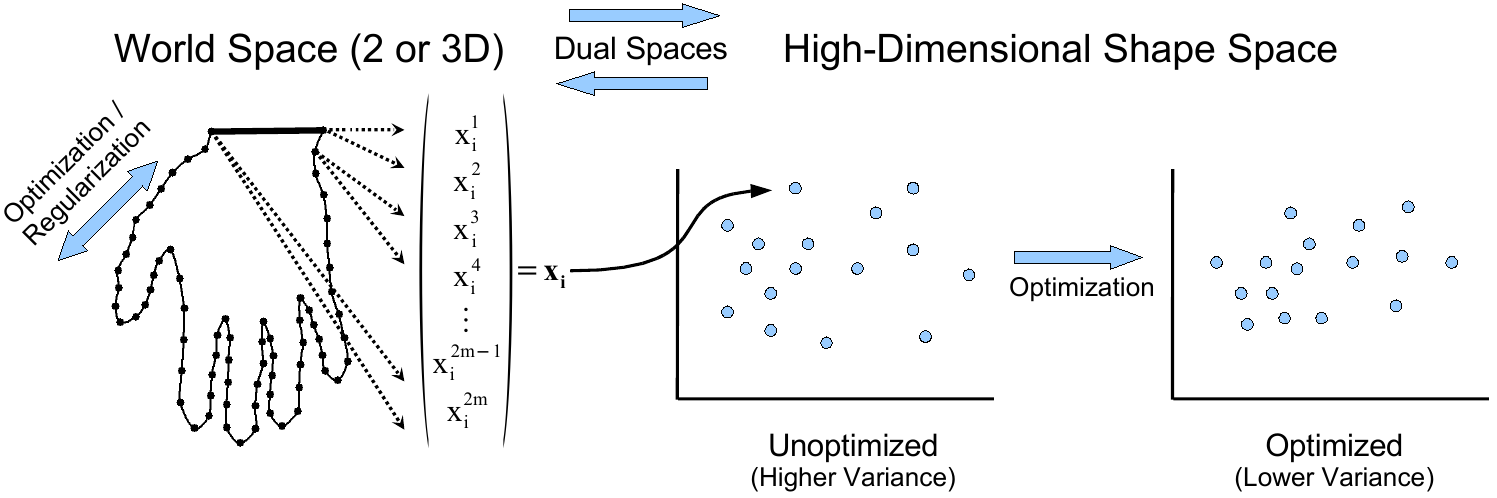
\includegraphics[width=0.9\textwidth]{figs_v2/overview.png}
	\caption{An illustration of the basic concepts the ShapeWorks point-based correspondence optimization.}
	\label{fig:overview}
\end{figure}


\subsection{Correspondence optimization}

The correspondence optimization currently implemented in ShapeWorks works by modeling the correspondence positions as sets of dynamic particles that are constrained to lie on the set of sample shape surfaces. The positions of the correspondences are optimized by gradient descent on an energy function that balances the negative entropy of the distribution of particles on each shape surface with the positive entropy of the distribution of the shape samples shape space. More specifically, and with reference to Fig \ref{fig:overview}, we consider $\mathbf{x}_k \in \mathbb{R}^{3m}$ as an instance of a random variable $\mathbf{Z}$ and minimize the energy function
\begin{equation}
Q =  \alpha H(\mathbf{Z}) -  \sum_k H(\mathbf{x}_k)
\end{equation}

\noindent where $H$ is an estimation of differential entropy. Minimizing the first term in $Q$ produces a compact distribution of samples in shape space, while the second term seeks uniform surface samplings for accurate shape representation. This latter term can also be modified to adaptively over-sample in response to local surface features such as curvature. The free parameter $\alpha$ balances the tradeoff between model compactness and accurate shape representation. Since correspondence points in this formulation are not tied to a specific parameterization, the method operates directly on volumetric data and extends easily to arbitrary shapes, even non-manifold surfaces.

\subsection{Shape modeling pipeline}

This software distribution consists of several applications that together make up a full processing pipeline for correspondence computation and visualization. The stages of the pipeline are as follows, (1) preprocessing, (2) alignment, (3) initialization, (4) optimization, and (5) visualization \& analysis. This section gives an overview of the steps involved in the pipeline. 

\vspace{0.1in}
\noindent\textbf{Preprocessing:} Any set of implicitly defined surfaces, such as a set of binary segmentations, is appropriate as input to this pipeline. By default, the software will assume a closed surface, but can also handle open boundaries (specified by cutting planes). % and non-manifold surfaces consisting of multiple closed surfaces.
A binary mask, such as the output of an image segmentation process, for example, contains an implicit shape surface at the interface of the labeled pixels and the background. Binary masks contain aliasing artifacts, however, that should first be removed. Typically we follow an antialiasing step with a very slight Gaussian blurring to remove the high-frequency artifacts that can occur as a result of numerical approximations.

\vspace{0.1in}
\noindent\textbf{Alignment:} A collection of shape segmentations must often be aligned in a common coordinate frame for modeling and analysis. The ShapeWorks software does not provide full support for this stage of the pipeline, since every new dataset may require a different process of alignment. Some basic alignment tools that are included with ShapeWorks are the ability to align the segmentations with respect to their centers of mass and the orientation of their first principal eigenvectors. For some classes of data, this method is effective as a rough alignment and is followed, during the optimization process, by iterative Procrustes alignments based on the correspondence point positions \cite{goodall1991procrustes}. ShapeWorks distinguishes between two separate coordinate frames: a local coordinate frame for each shape sample, and a common coordinate frame in which all shape samples are co-registered. For applications in which the input data is completely registered, these two coordinate frames are the same. Where there is a distinction, ShapeWorks will maintain and output appropriate transformations to the common coordinate frame for each shape sample, as well as separate correspondence files for each coordinate frame.

\vspace{0.1in}
\noindent\textbf{Correspondence initialization:} Typically, we initialize the correspondence optimization with a single particle that finds the nearest zero of the implicit surface, and then splits under optimization (producing a new, nearby particle) at regular intervals until a specific number of particles are produced and reach a steady state. This initialization procedure is supported within ShapeWorks and its Studio software. We have found this procedure to be generally applicable to classes of closed shapes with reasonably smooth surfaces. %For more complicated shapes, it may be necessary to specify initial particle positions for the optimization using other means. Initial particle positions may be computed offline and supplied to ShapeWorks as a text file input (see Section 3.2).

\vspace{0.1in}
\noindent\textbf{Correspondence optimization:} The optimization stage proceeds as described earlier starting with an initial set of particle positions and a set of implicit surfaces (e.g., signed distance transforms). Several types of optimization procedures are supported: adaptive gradient descent, Jacobi updates, and Gauss-Seidel updates. By default, gradient descent with Gauss-Seidel updates is used. Important parameters to consider for the optimization are the regularization on the covariance matrix for the shape-space entropy estimation, and the parameter $\alpha$ from Equation 1 which controls the trade-off between the uniformity of the surface sampling and the compactness of the optimized model. Also consider whether iterative Procrustes alignment is necessary and how often to it can be performed. %and whether or not to remove Procrustes scale from the correspondence model.

\vspace{0.1in}
\noindent\textbf{Visualization and analysis:} Statistical analysis of point-based shape models is difficult because point-wise statistical tests require multiple-comparisons corrections that significantly reduce statistical power \cite{cates2008hypothesis}. Analysis in the full shape space, however, is problematic due to the high number of dimensions and the difficulty of obtaining sufficient samples. A common solution is to employ dimensionality reduction reduction by choosing a subspace in which to project the data for traditional multivariate analysis (see, e.g., \cite{cates2008particle,cates2008hypothesis}). This software does not include specific code for statistical analysis of the correspondences. It does, however, provide principal component analysis (PCA), which can be used for dimensionality reduction prior to subsequent statistical analysis, and visualization of orthogonal modes of variation in the model (see, e.g,. \cite{cates2008particle,cates2008hypothesis}). ShapeWorks also includes methods for computing and visualizing the Euclidean mean shapes and the median shapes of populations. Typically, we use a separate statistical package, such as R (the R Foundation, www.r-project.org), for analysis of the PCA loadings of the correspondence positions. The user-friendly Studio package provides tools to export different optimization outputs for subsequent statistical analysis. For more ideas regarding visualization and statistical analysis of correspondence models, see the various publications listed in the bibliography section of this document.


\section{Documentation}
For documentation, please see: \texttt{http://sciinstitute.github.io/shapeworks.pages}

\section{Sample datasets}

Studio's release page\footnote{\texttt{https://github.com/SCIInstitute/ShapeworksStudio/releases}} contains links to the following datasets.

\begin{itemize}
	\item [-] \textbf{Ellipsoid dataset:} 9 binary image volumes of pre-aligned ellipsoids with varying major radius (i.e. one dominant mode).
		\item [-] \textbf{Torus dataset:} 20 binary image volumes of pre-aligned tori with varying inner and outer radii (i.e. two dominant modes). This dataset contains a couple of thin tori whose geometries are affected by the Gaussian blurring sigma (in the Groom stage), best sigma setting would be 2.
		\item [-] \textbf{Torus subset dataset:} 10 binary image volumes of pre-aligned tori with varying inner and outer radii (i.e. two dominant modes). This dataset can be used to quickly test parameter settings for the full torus dataset.
		\item [-] \textbf{Femur dataset:} 10 binary image volumes of roughly pre-aligned healthy femurs with a cutting plane to limit particles distribution above the lesser trochanter.
\end{itemize} 


\section{System requirements}

\subsection{Minimum recommended system configuration:}
\begin{itemize}
	\item[-] Windows 7+, OSX 10.9+, and OpenSuse 13.1+ Recommended. Other platforms may work, but are not officially supported.
		\item[-] CPU: Core Duo or higher, recommended i5 or i7
	\item[-] 	Memory: 4Gb, recommended 8Gb or more
	\item[-] 	Graphics Memory: minimum 128MB, recommended 256MB or more
\end{itemize}

\subsection{Windows}
The current source code must be compiled with the 64-bit version of Visual Studio 2015.

\subsection{Mac OS X}
The source code base was built with Xcode as well as GNU Make and works for both environments on OS X 10.9+.

\subsection{Linux specifications}
The code base has been tested for use with GCC, and this is the recommended compiler for linux. Compiler must support C++11.

\subsection{Build from source}
ShapeworksStudio can be (compiled) from source on Linux platforms (OpenSuSE, Ubuntu etc.), OSX, and Windows. It requires at least the following:
\begin{itemize}
\item[-] C++11 64-bit compatible compiler
\item[-] Git 1.8 or higher (https://git-scm.com/)
\item[-] CMake 2.8+ (http://www.cmake.org/)
\item[-] Visualization ToolKit (VTK 7.* recommended) (http://www.vtk.org/)
\item[-] Insight Toolkit (ITK 4.7+ recommended) (http://www.itk.org/)
\item[-] Qt 5.* (http://www.qt.io/developers/)
\item[-] NVIDIA card and drivers for Linux
\item[-] Graphics cards must support OpenGL 2.0 or greater (not available on older Intel embedded graphics cards).
\end{itemize}

\noindent Consult the distribution-specific section for additional package information and the developer documentation for build instructions.

\subsection{OpenSuSE}

We are currently testing on 64-bit Leap 42.1 (OpenSuSE package repository information). OpenSuSE RPMs: gcc, gcc-c++, Make, CMake, git, glu-devel, libXmu-devel, CMake-gui, CMake.

\section{ Build instructions}

\subsection{Dependencies}

ShapeWorks and ShapeWorksStudio software depends on several open-source, freely-available software toolkits. To build the full set of tools, including the graphical interfaces, you will need the following packages.

\noindent\textbf{Qt:} Qt binaries and packages are available on the Qt website or can be built from source code. Gcc/Clang/MSVC with C++11 support is required.\\
\textbf{CMake:} CMake versions 2.8 - 3.4 are supported.\\
\textbf{ITK:} ITK Insight Toolkit (ITK 4.7+ recommended)\\
\textbf{VTK:} VTK Visualization ToolKit (VTK 7. recommended)\\

\subsection{Supported platforms}

ShapeWorks and ShapeWorksStudio softwares are written ANSI C++ code and has been built successfully on Windows 64-bit, Mac OS X, and Linux 64-bit. Any platform for which ITK, VTK, and Qt are supported should, in theory, also support the ShapeWorks and ShapeWorksStudio softwares.


\subsection{Binary distributions}

Binary distributions of ShapeWorksStudio software for Windows 64-bit and Mac OS X platforms are also available for download\footnote{\texttt{https://github.com/SCIInstitute/ShapeworksStudio/releases}}. Unless you intend to do development with the ShapeWorks source code, it is highly recommended that you use a binary distribution, if one is available for your system.


\subsection{Compiling dependencies from source}

Once you have obtained a compatible compiler and installed Qt on your system, you need to download and install CMake (http://www.cmake.org) to actually build the software. CMake is a platform independent configuring system that is used for generating Makefiles,Visual Studio project files, or Xcode project files.

\vspace{0.6in}
\noindent\textbf{Compiling ITK:} 

Configure with:
\begin{lstlisting}[style=BashInputStyle]
CMAKE_CXX_FLAGS+="-std=c++11"
BUILD_SHARED_LIBS=FALSE
BUILD_EXAMPLES=FALSE
BUILD_TESTING=FALSE
ITKV3_COMPATIBILTY=TRUE
\end{lstlisting}

Then build ITK.

\begin{lstlisting}[style=BashInputStyle]
make -j12 all
\end{lstlisting}

You may need to use the CMake GUI in Windows. It is best to configure with “NMake Makefiles”. Once you have configured and generated, you can build in a command prompt.

\begin{lstlisting}[style=BashInputStyle]
cd Path/To/Your/ITK
mkdir build
cd build
nmake all
\end{lstlisting}

\vspace{0.1in}
\noindent\textbf{Compiling VTK:}

Configure with:

\begin{lstlisting}[style=BashInputStyle]
VTK_Group_Qt=ON
VTK_QT_VERSION=5
Qt5_DIR="/PATH/TO/YOUR/Qt5
BUILD_SHARED_LIBS=FALSE
BUILD_EXAMPLES=FALSE
BUILD_TESTING=FALSE
\end{lstlisting}

Then build VTK. Note: Be sure that you are linking VTK with the same Qt5 Library you are using to build Studio.

\begin{lstlisting}[style=BashInputStyle]
make -j12 all
\end{lstlisting}

You may need to use the CMake GUI in Windows. It is best to configure with “NMake Makefiles”. Once you have configured and generated, you can build in a command prompt.

\begin{lstlisting}[style=BashInputStyle]
cd Path/To/Your/VTK
mkdir build
cd build
nmake all
\end{lstlisting}

\subsection{Compiling ShapeworksStudio from source}

Once CMake, Qt, ITK, and VTK have been installed and/or built, run CMake from your build directory and give a path to the ShapeworksStudio directory containing the master CMakeLists.txt file.

\vspace{0.1in}
\noindent\textbf{Unix and OSX:}

\begin{lstlisting}[style=BashInputStyle]
mkdir ShapeWorksStudio/build
cd ShapeWorksStudio/build
cmake -DVTK_DIR=Path/To/Your/VTK/build -DITK_DIR=Path/To/Your/ITK/build -DQT_DIR=Path/To/Your/Qt5/build -DCMAKE_BUILD_TYPE=Release ../src
make
\end{lstlisting}

Depending on how you obtained Qt, you may need to specify other Qt directories:

\begin{lstlisting}[style=BashInputStyle]
-DQT5WidgetsDIR=Path/To/Qt/5.6/gcc/lib/cmake/Qt5Widgets
-DQT5OpenGLDIR=Path/To/Qt/5.6/gcc/lib/cmake/Qt5OpenGL
\end{lstlisting}

\vspace{0.1in}
\noindent\textbf{Windows:} Open a Visual Studio 64 bit Native Tools Command Prompt. Follow these commands:

\begin{lstlisting}[style=BashInputStyle]
mkdir Path/To/ShapeWorksStudio/build
cd Path/To/ShapeWorksStudio/build
cmake -G "NMake Makefiles" -DVTK_DIR=Path/To/Your/VTK/build -DITK_DIR=Path/To/Your/ITK/build -DQT_DIR=Path/To/Your/Qt5/build -DCMAKE_BUILD_TYPE=Release ../src
nmake
\end{lstlisting}

\noindent NOTE: Be sure to copy the Qt5 DLL files to the Executable directory for the program to run.

\begin{lstlisting}[style=BashInputStyle]
Path/To/Your/Qt5/build/msvc2015/5.6/bin/Qt5Widgets.dll
Path/To/Your/Qt5/build/msvc2015/5.6/bin/Qt5Core.dll
Path/To/Your/Qt5/build/msvc2015/5.6/bin/Qt5OpenGL.dll
Path/To/Your/Qt5/build/msvc2015/5.6/bin/Qt5Gui.dll
\end{lstlisting}

\vspace{0.1in}
\noindent\textbf{All platforms:} Your paths may differ slightly based on your Qt5, ITK, and VTK versions and where they are installed/built. The console version ccmake, or GUI version can also be used. You may be prompted to specify your location of the Qt installation. If you installed Qt in the default location, it should find Qt automatically. After configuration is done, generate the make files or project files for your favorite development environment and build. The ShapeworksStudio application will be built in bin/Application.
\vspace{0.1in}
\begin{figure}[!htp]
	\centering
	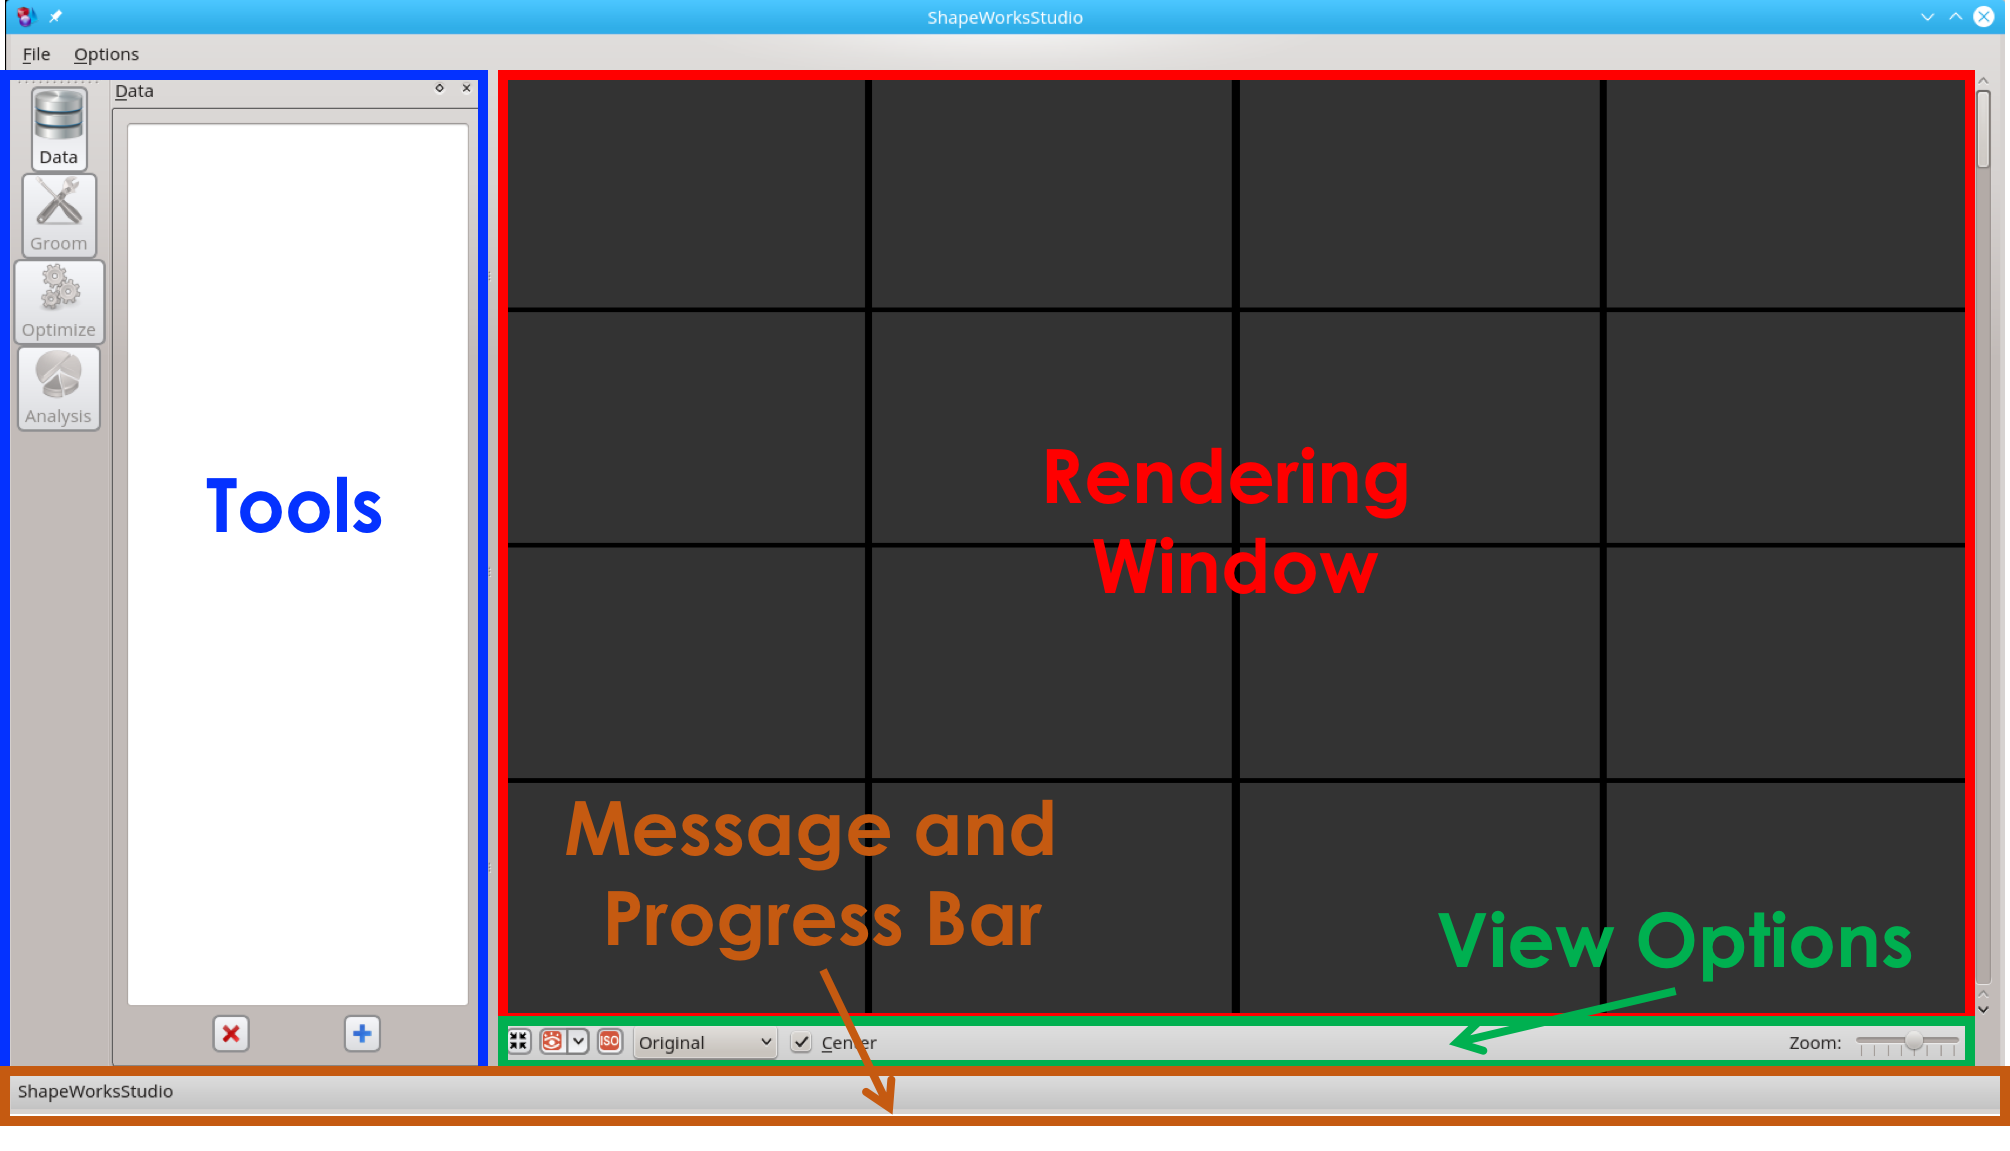
\includegraphics[width=0.9\textwidth]{figs_v2/qtwin.png}
	\caption{Initial ShapeWorksStudio window}
	\label{fig:qtwin}
\end{figure}

\section{Running ShapeWorksStudio}

Studio runs with no command-line arguments. Double click the generated binary file in Windows/Mac or use \texttt{./ShapeWorksStudio} on Linux terminal.  You should have a Qt window that looks similar to the one shown in Fig. \ref{fig:qtwin}. The application has tools on the left, a rendering window, view options on the lower bar, a file menu, and a preferences dialog. Studio messages and progress can be monitored using the bar at the very bottom. It is also recommended to run Studio's binary from a terminal/console in order to monitor the detailed output log of Studio while it is running different stages.

\section{File formats}

%\vspace{0.1in}
\noindent\textbf{Image volumes:} Inputs to ShapeWorksStudio are surfaces embedded in image volumes. ShapeWorks can read and write any image file format supported by the Insight Toolkit. ShapeWorksStudio currently supports NRRD and MHA file formats. For the optimization step, shape surfaces must be represented implicitly as the zero level set of a signed distance transform.

\vspace{0.1in}
\noindent\textbf{Point files:} Correspondence point positions are stored in plain text files. These files contain no header, and are simply a list of the point positions written as follows 

\noindent\texttt{x1 y1 z1}\\
\noindent\texttt{x2 y2 z2}\\
... \\
\noindent\texttt{xm ym zm}

\noindent where \texttt{x y z} are floating point numbers and \texttt{m} is the number of correspondence points. Two point files are maintained for each shape. The first has file extension \texttt{.lpts}, and is the correspondence positions in that shape’s local coordinate space. The second file has extension \texttt{.wpts}, and is the correspondence positions in the common (world) coordinate space. The \texttt{.lpts} files can be used to initialize particles on shape surfaces for optimization, while the \texttt{.wpts} files should be used for any statistical analysis.

\vspace{0.1in}
\noindent\textbf{Parameter files:} ShapeWorksStudio is a project-based graphical user interface (GUI) that uses a well-defined XML project file format specification to support checkpointing, managing/sharing input/output files, restarting optimizations at checkpoints, and offloading the data preprocessing and/or the model optimization to an external machine.
\vspace{0.2in}

\begin{figure}[!htp]
	\centering
	
\includegraphics[width=0.9\textwidth]{figs_v2/add.png}
	\caption{Import binary volumes using the blue "+" button}
	\label{fig:add}
\end{figure}

\begin{figure}[!htp]
	\centering
	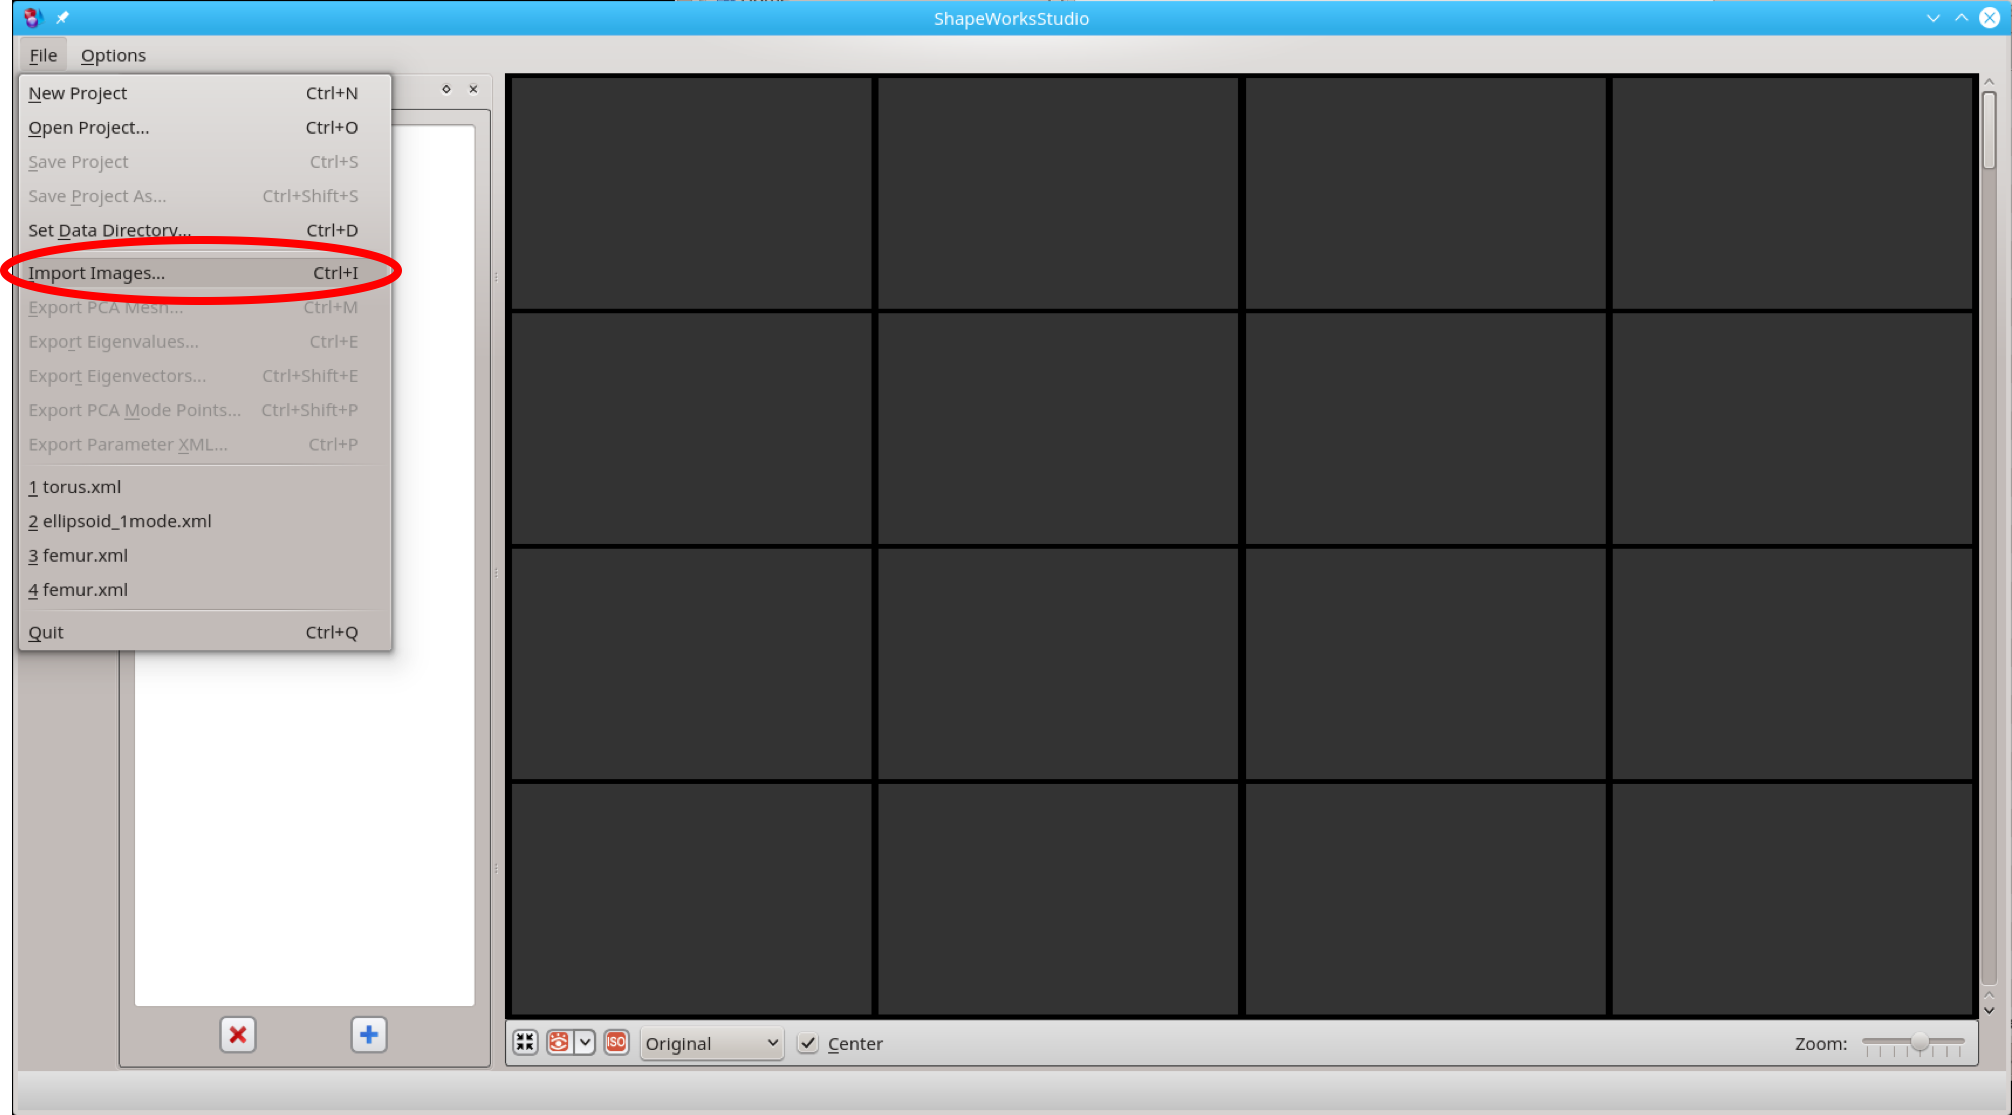
\includegraphics[width=0.9\textwidth]{figs_v2/import.png}
	\caption{Import binary volumes from the file menu}
	\label{fig:import}
\end{figure}

\begin{figure}[!htp]
	\centering
	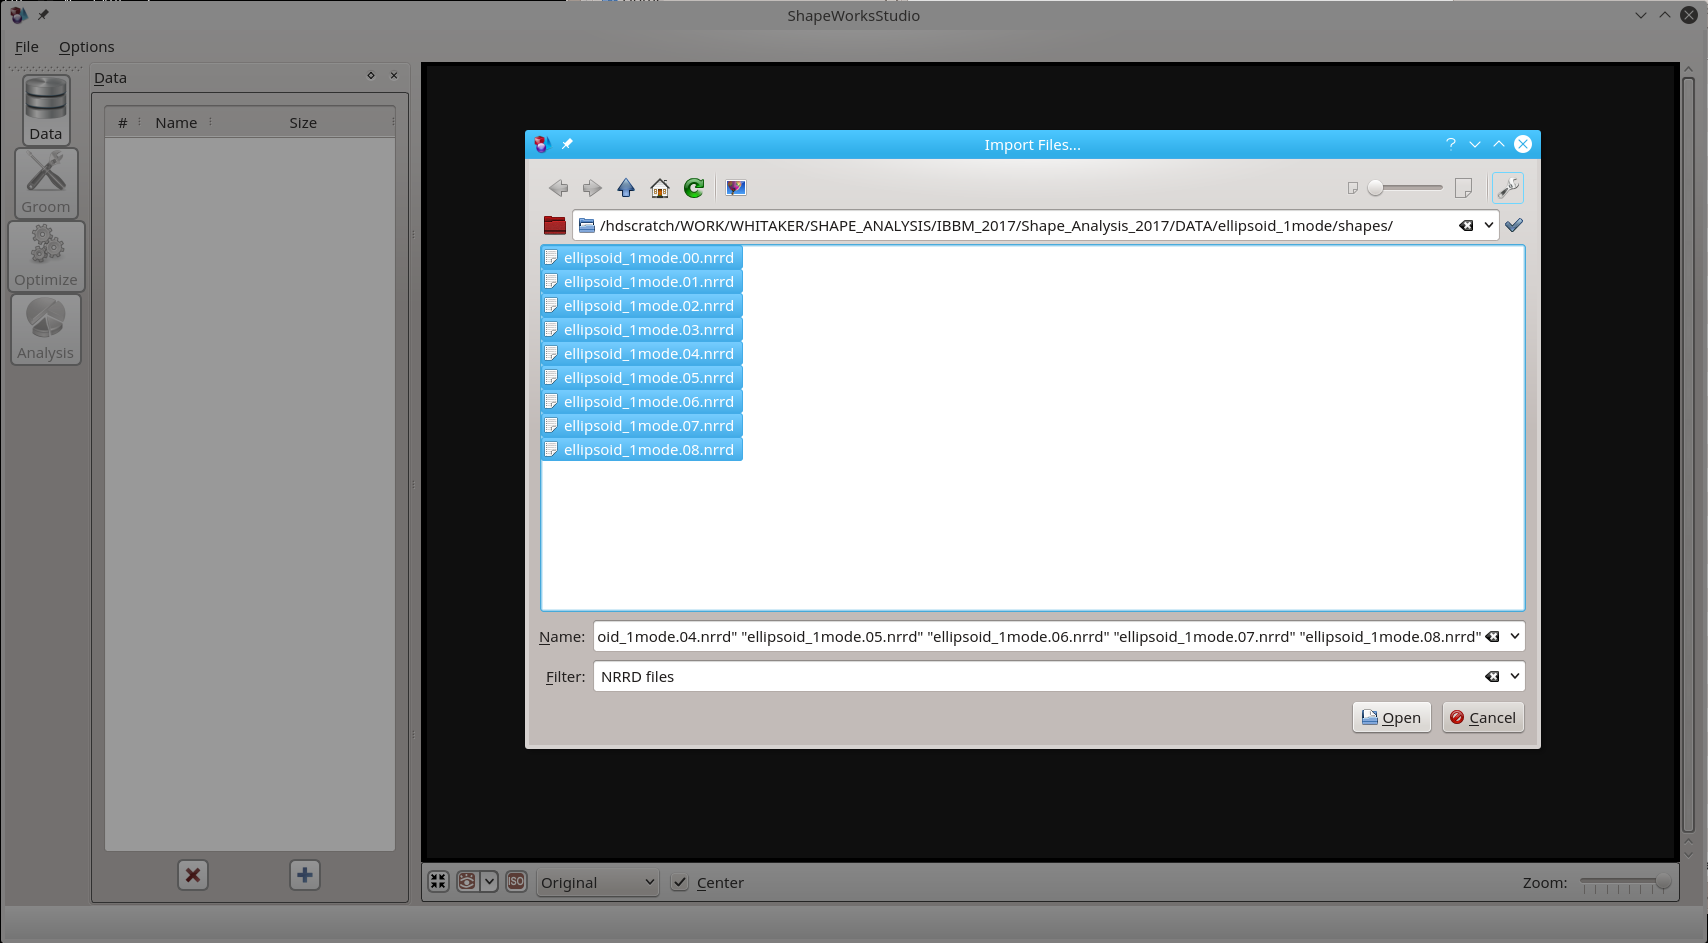
\includegraphics[width=0.9\textwidth]{figs_v2/imagefiles.png}
	\caption{Selection of multiple files to be loaded to your studio project}
	\label{fig:imagefiles}
\end{figure}

\begin{figure}[!htp]
	\centering
	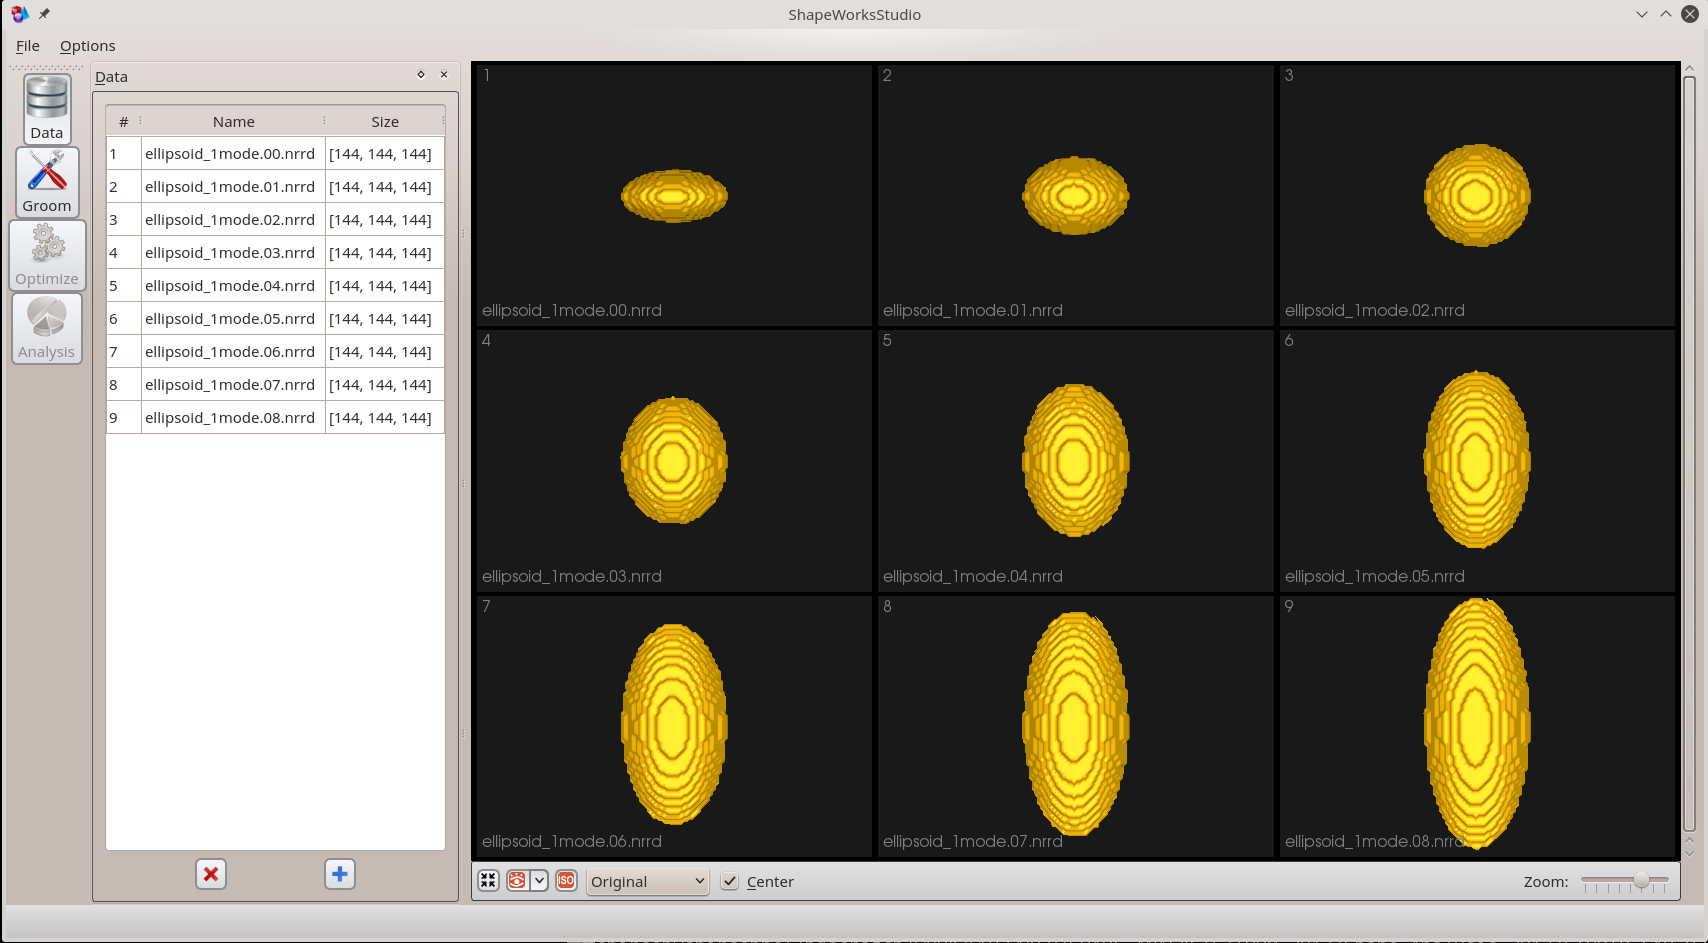
\includegraphics[width=0.9\textwidth]{figs_v2/ellipsoid_images.png}
	\caption{After loading the images: Left: the \texttt{Data} panel shows the files names and the image sizes. Right: the rendering window displays the isosurface of the binary images that have been loaded to your project}
	\label{fig:ellipsoid_images}
\end{figure}

\begin{figure}[!htp]
	\centering
	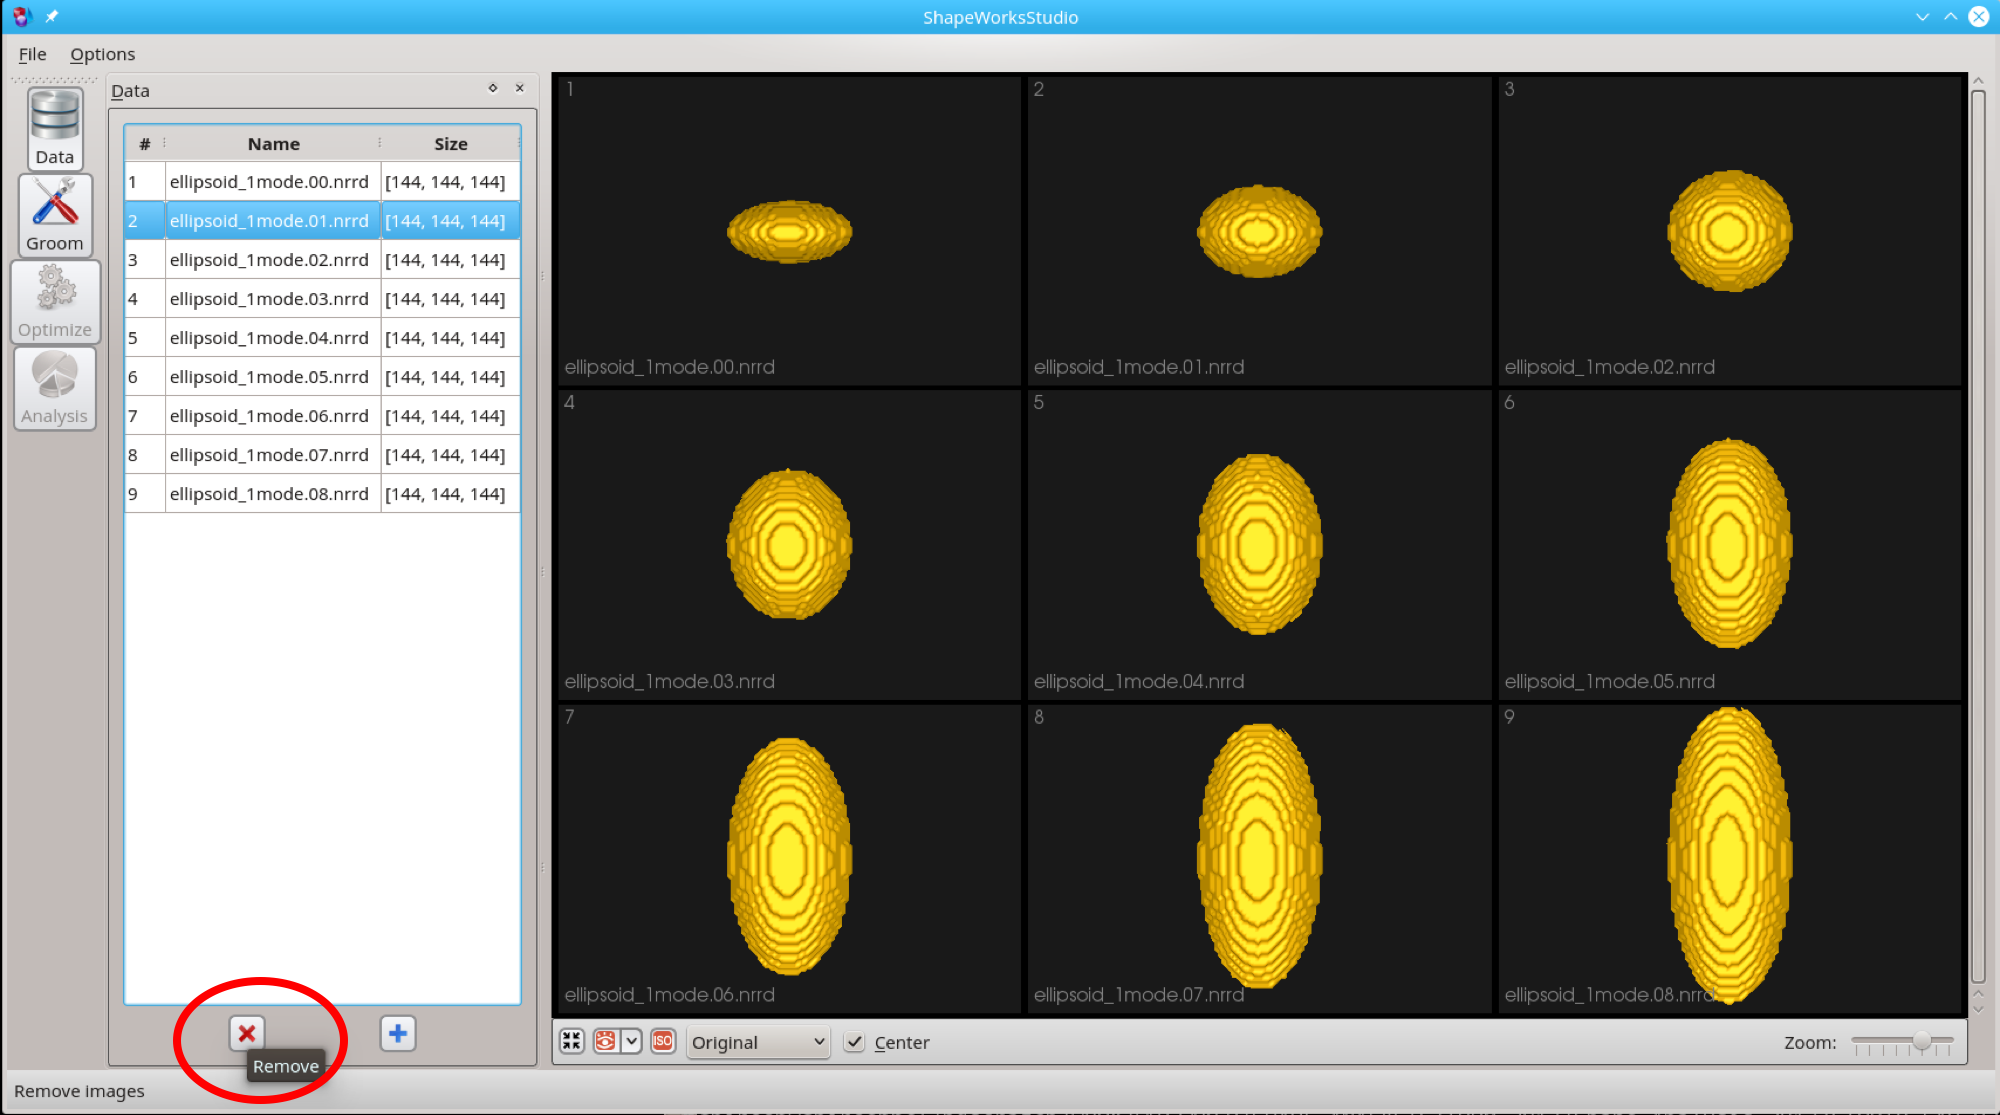
\includegraphics[width=0.9\textwidth]{figs_v2/remove.png}
	\caption{At any time, you can select an image to be removed from your project using the red "x" button}
	\label{fig:remove}
\end{figure}


\section{Tools}

\subsection{Data}

\noindent\textbf{Imorting your data:} This \texttt{Data} panel displays the images (volume files in NRRD or MHA format) that have been loaded. You can select the image files to load by either clicking the blue "+" button at the bottom (see Fig. \ref{fig:add}), or going to \texttt{File -> Import Images} (see Fig. \ref{fig:import}). Once the file import dialog appears, you can select multiple files to be loaded to your Studio project (see Fig. \ref{fig:imagefiles}). Your images will appear on the display once loaded (see Fig. \ref{fig:ellipsoid_images}). You can delete images by selecting the image of choice and clicking the red "x" button at the bottom (see Fig. \ref{fig:remove}). 

\vspace{0.1in}
\noindent\textbf{Saving your project:} It is recommended to continuously save your project by pressing \texttt{Ctrl+S} or using the file menu (see Fig. \ref{fig:save}) in order to be able to resume your project after closing the current session. By default, Studio saves the current project in the directory from which you loaded your images. In order to change the output directory, use \texttt{File -> Set Data Directory} (see Fig. \ref{fig:setdir})  to set the data directory for where generated images will be written when your project is saved. Note that in case you want to change the path of the current project or saving it as a new project (using \texttt{File -> Save Project As}), you need to set the data directory to the new path such that all Studio output will be saved in this path. This is helpful in case you wanted to save Studio output for different combination of parameter settings. Studio is smart enough to ask you to save your project upon leaving (see Fig. \ref{fig:close}). Studio project file is an xml file containing the list of images being imported to your project and the corresponding files generated from different stages (i.e. grooming, optimization and analysis). \vspace{0.2in}

\begin{figure}[!htp]
	\centering
	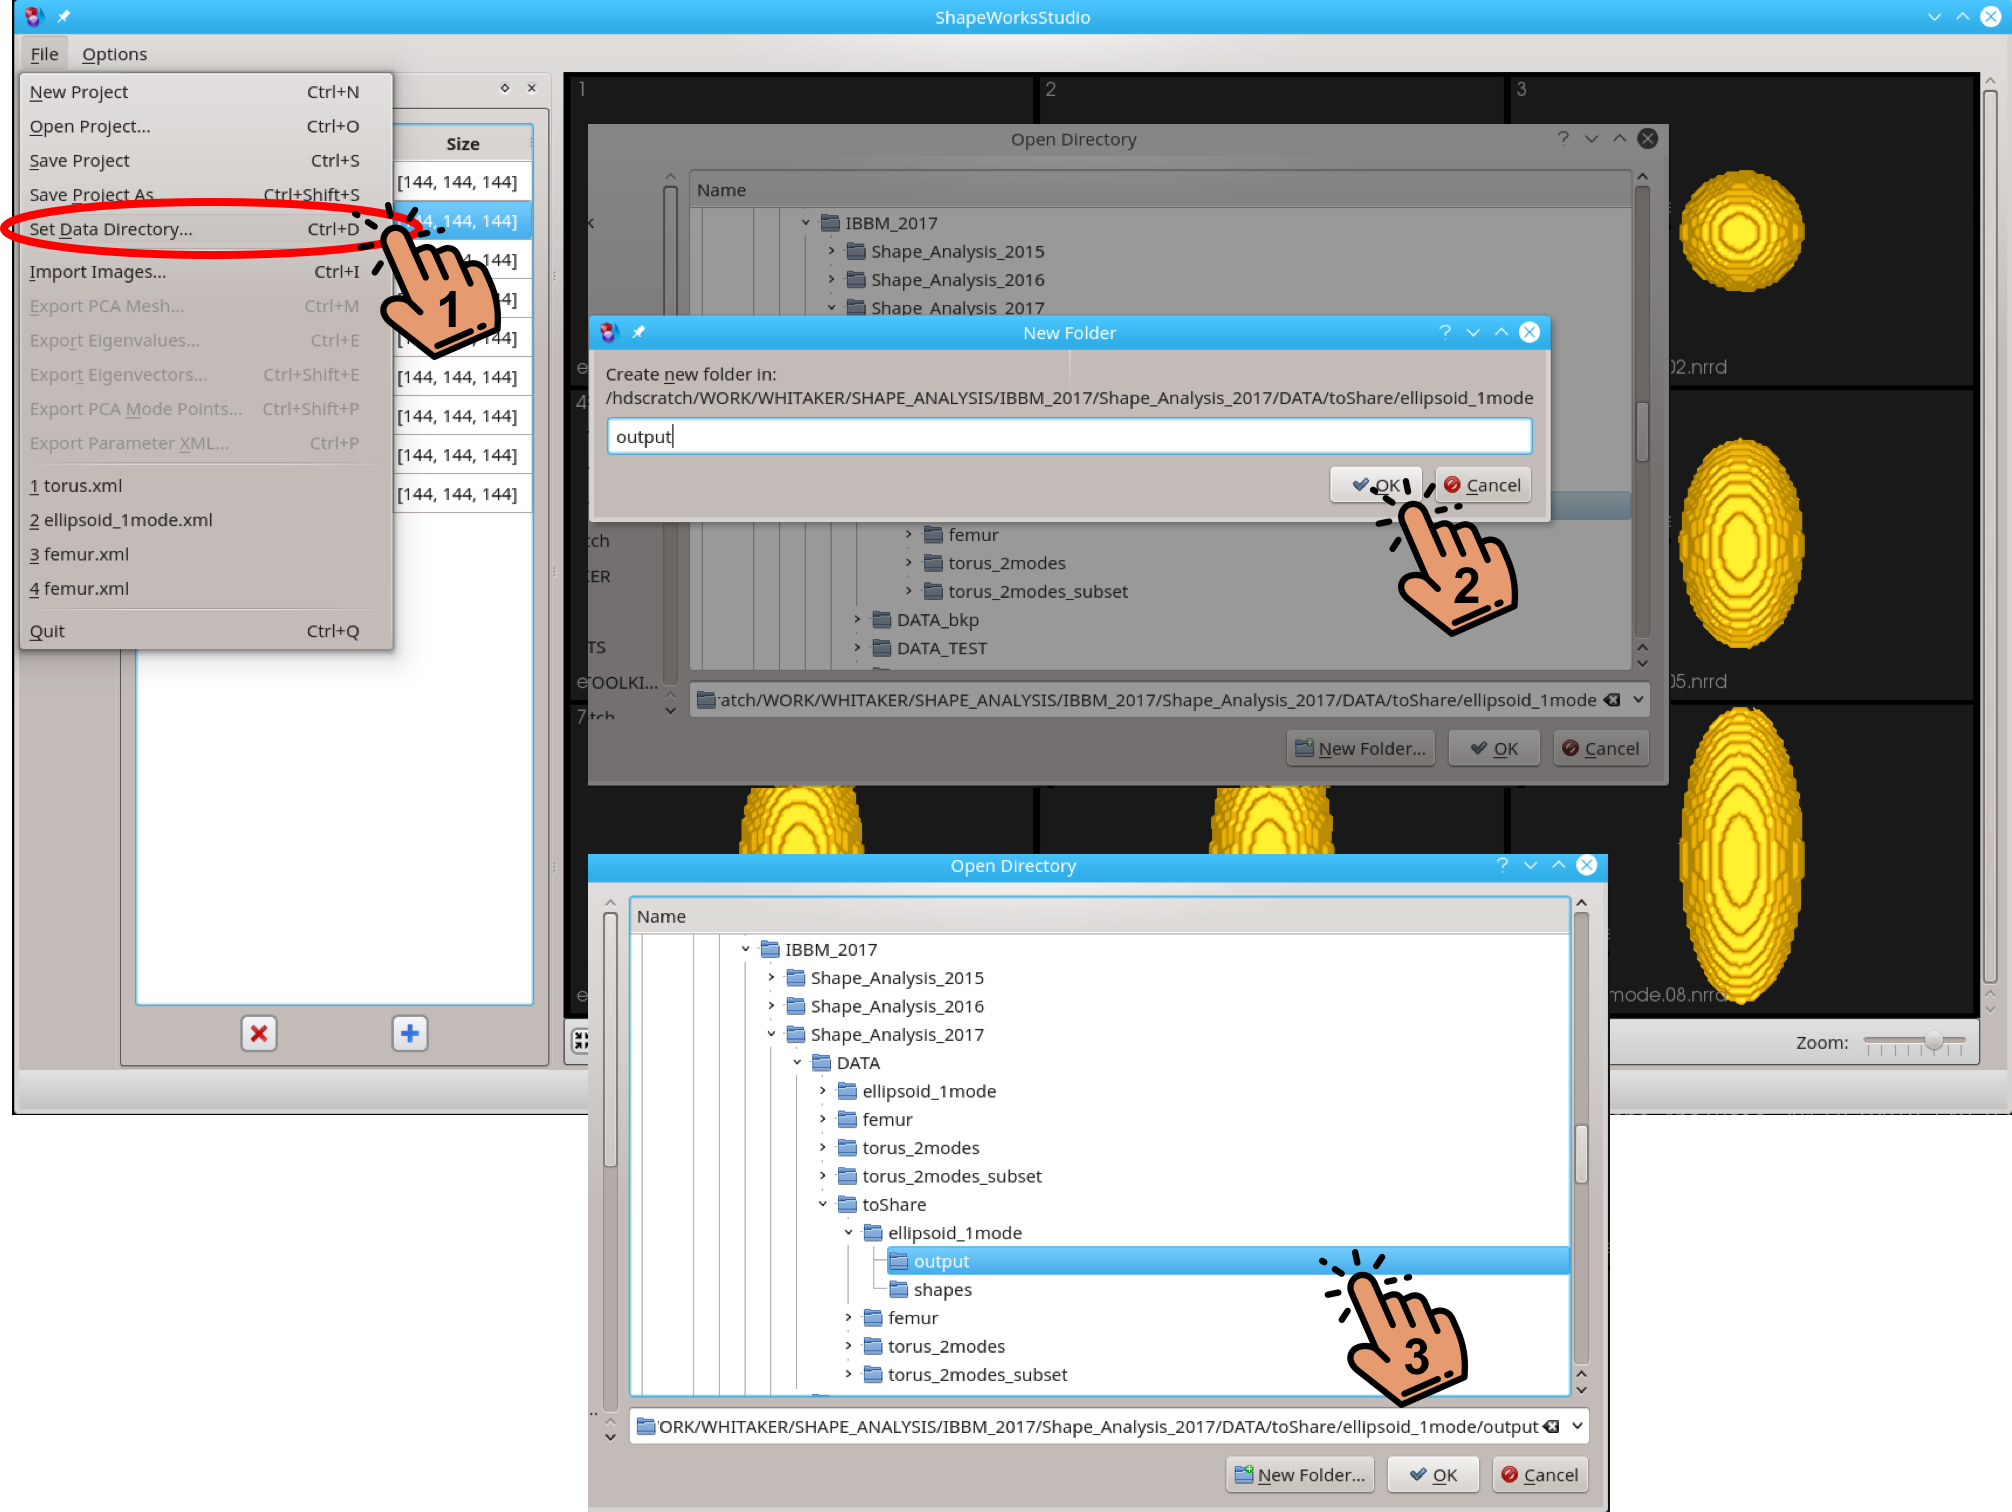
\includegraphics[width=0.9\textwidth]{figs_v2/set_dir.png}
	\caption{Setting data directory}
	\label{fig:setdir}
\end{figure}

\begin{figure}[!htp]
\centering
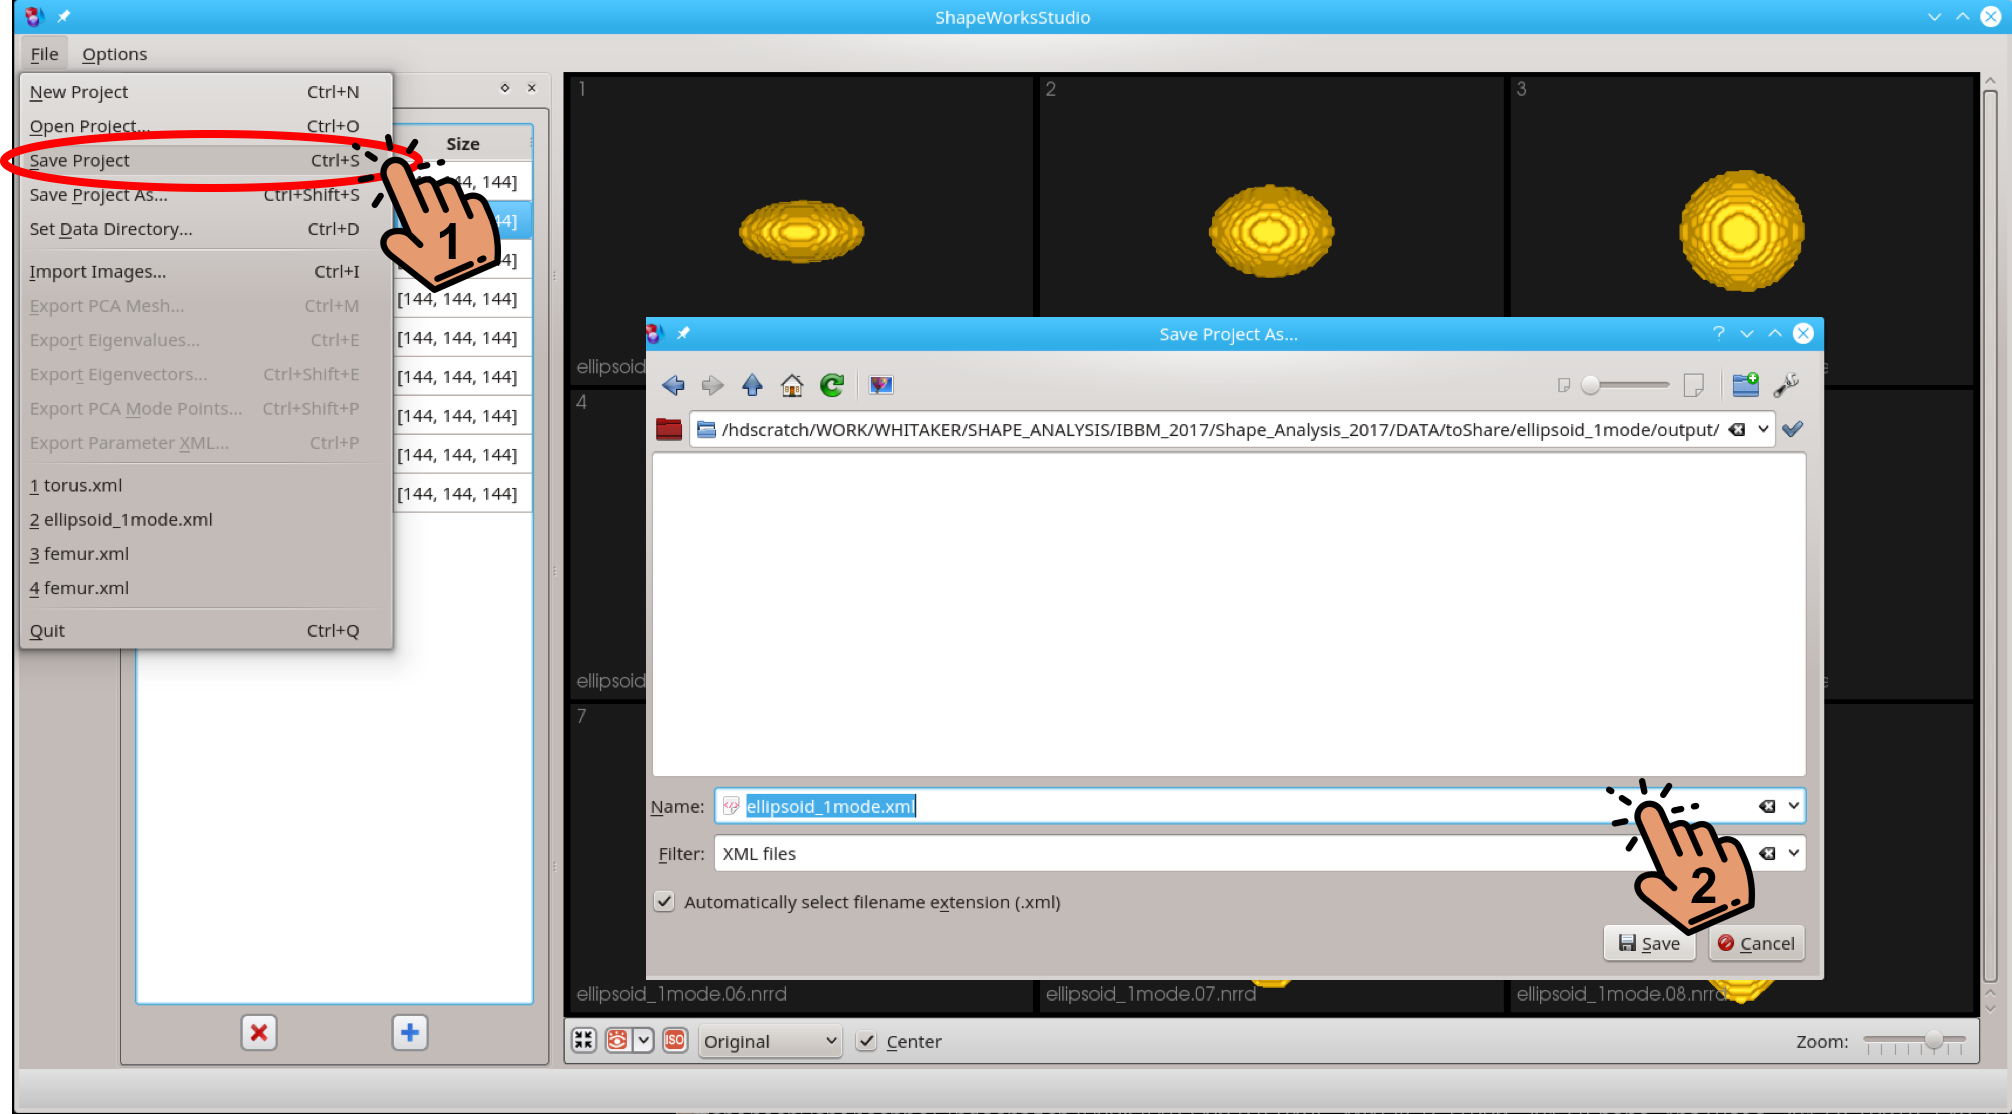
\includegraphics[width=0.9\textwidth]{figs_v2/save.png}
\caption{Saving your project}
\label{fig:save}
\end{figure}

\begin{figure}[!htp]
\centering
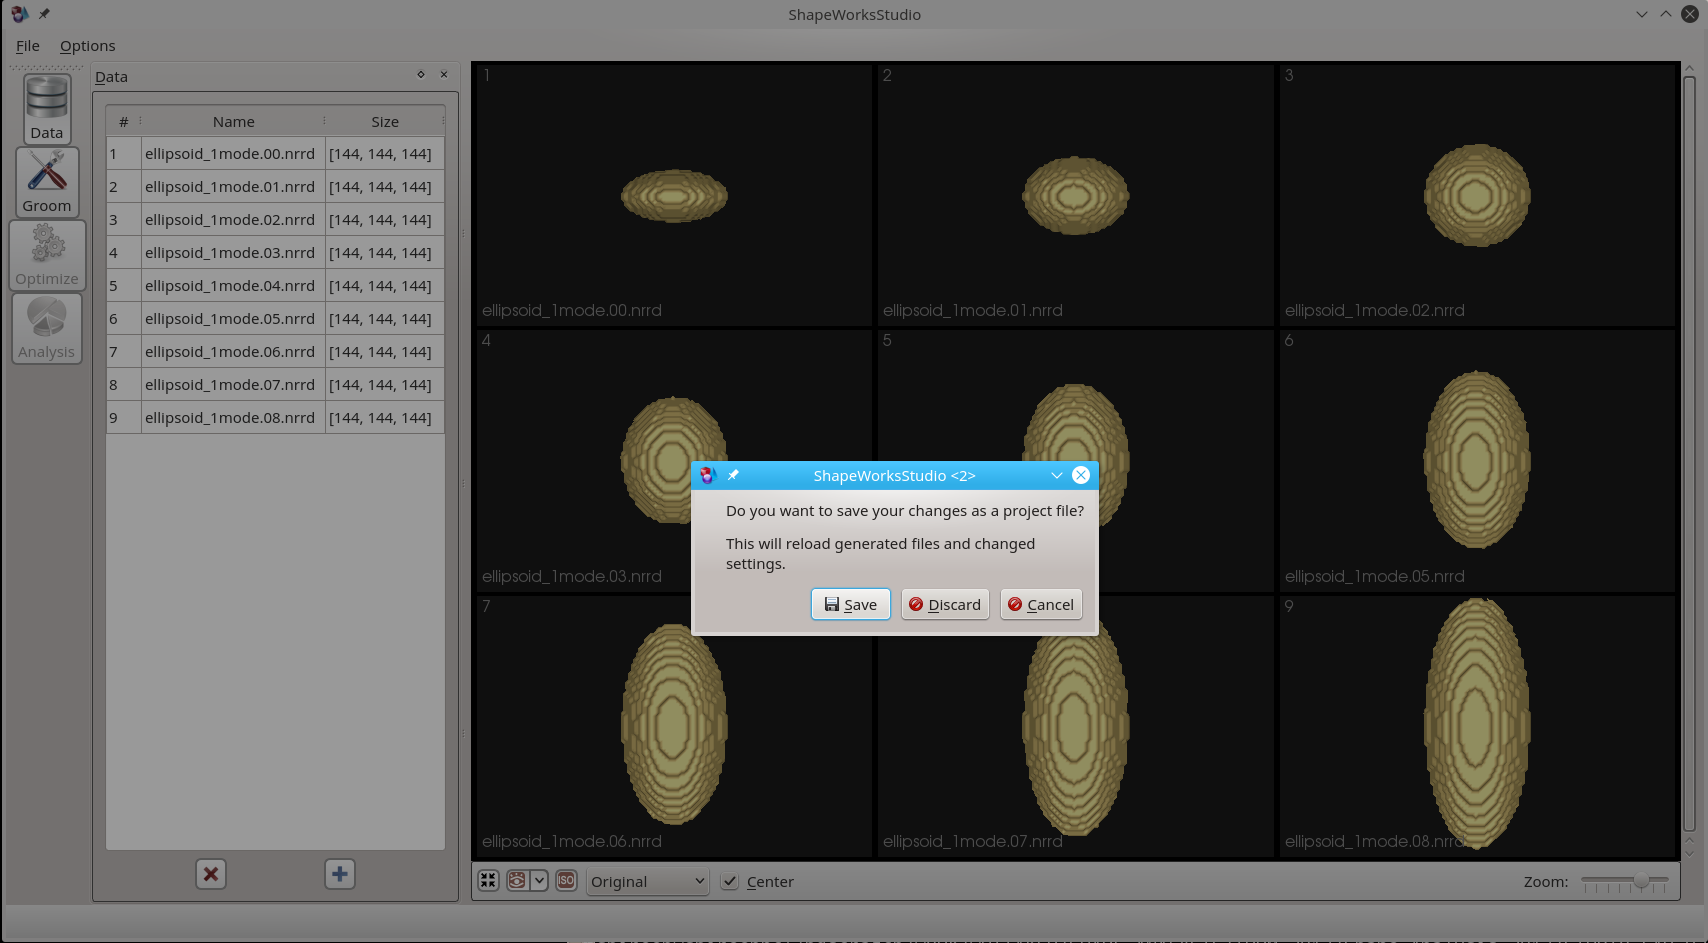
\includegraphics[width=0.9\textwidth]{figs_v2/close.png}
\caption{Studio asks you to save your project upon closing}
\label{fig:close}
\end{figure}

\vspace{0.05in}
\begin{figure}[!htp]
	\begin{minipage}[c]{0.6\textwidth}
		\centering
		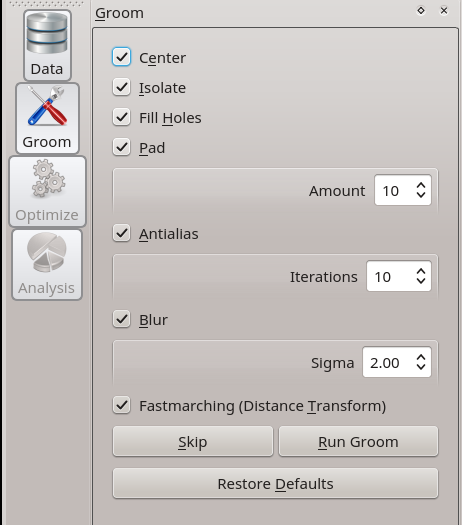
\includegraphics[width=0.8\textwidth]{figs_v2/groom.png}
	\end{minipage}\hfill
	\begin{minipage}[c]{0.3\textwidth}
		\centering
		\caption{\texttt{Groom}-ing your shapes is a preprocessing step that would convert the input binary images to their corresponding implicit representation for ShapeWorks while taking care of aliasing artifacts} 
		\label{fig:groom}
	\end{minipage}
\end{figure}

\subsection{Groom}

Once more than 1 image is loaded, the preprocessing step, \texttt{Groom} is next. Its primary purpose is to convert binary, volumetric image segmentations (label masks) into distance transforms that are suitable for input to the correspondence optimization step. Filtering operations are implemented using ITK (The Insight Toolkit), and are applied in batch processing mode. Some of the filtering operations that Studio supports are antialiasing, hole-filling, smoothing, and distance transforms. You can select several options for grooming (see Fig. \ref{fig:groom}).

\begin{itemize}
\item[-] \textbf{Center:} This option attempts to align the segmentations to a common center if they are not the same sizes.
\item[-] \textbf{Isolate:} This option isolates the foreground (non-zero voxels) from the background.
\item[-] \textbf{Fill Holes:} This option fills any existing holes in the loaded segmentations.
\item[-] \textbf{Pad:} This option adds a padding around the shapes. This is helpful when the segmentations are very close to or touching the volume boundaries. Padding the volumes would help the optimization step to keep the particles within the volume boundaries without shooting the particles outside, especially at high curvature regions. The selected padding amount is the number of voxels to be padded in each dimension.
\item[-] \textbf{Antialias:} This option antialiases the binary segmentation in order to remove the staircase effect at shapes' isosurfaces resulting from the abrupt change of a binary image between a background and a foreground voxel. The resulting antialiased volumes will have a smooth transition between foreground and background regions. You can select the number of antialias iterations with more iterations resulting in a smoother transition.
\item[-] \textbf{Blur:} This option blurs the resulting distance transforms to get rid of high-frequency artifacts. You can choose an appropriate sigma for the blurring with higher sigma values resulting in smoother surfaces. Sigma values are relative to the images spacing (i.e., voxel size). It is recommended not to use high values of sigma that would erode (remove/affect) thin structures in your shapes.
\item[-] \textbf{Fastmarching:} This option computes a signed distance transform of the surface using the Fast Marching method.
\item[-] \textbf{Run Groom:} Click this when you are ready for grooming. This step takes some time. You can monitor the output messages on the terminal or refer to ShapeWorksStudioTools.log file next to the executable. A progress indicator shows the tool is working (see Fig. \ref{fig:grooming}). In case you are not satisfied with the groomed shapes, e.g., too smooth, you can always modify any of the aforementioned parameters and click "Run Groom" again.
\item[-] \textbf{Skip:} Click this if you believe your data to already be pre-processed to your liking. This is helpful in case you have a set of distance transforms to be loaded directly from previously preprocessed segmentations.
\item[-] \textbf{Restore Defaults:} Click this to restore all parameter values to their program defaults. 
\end{itemize}

\begin{figure}[!htp]
	\centering
	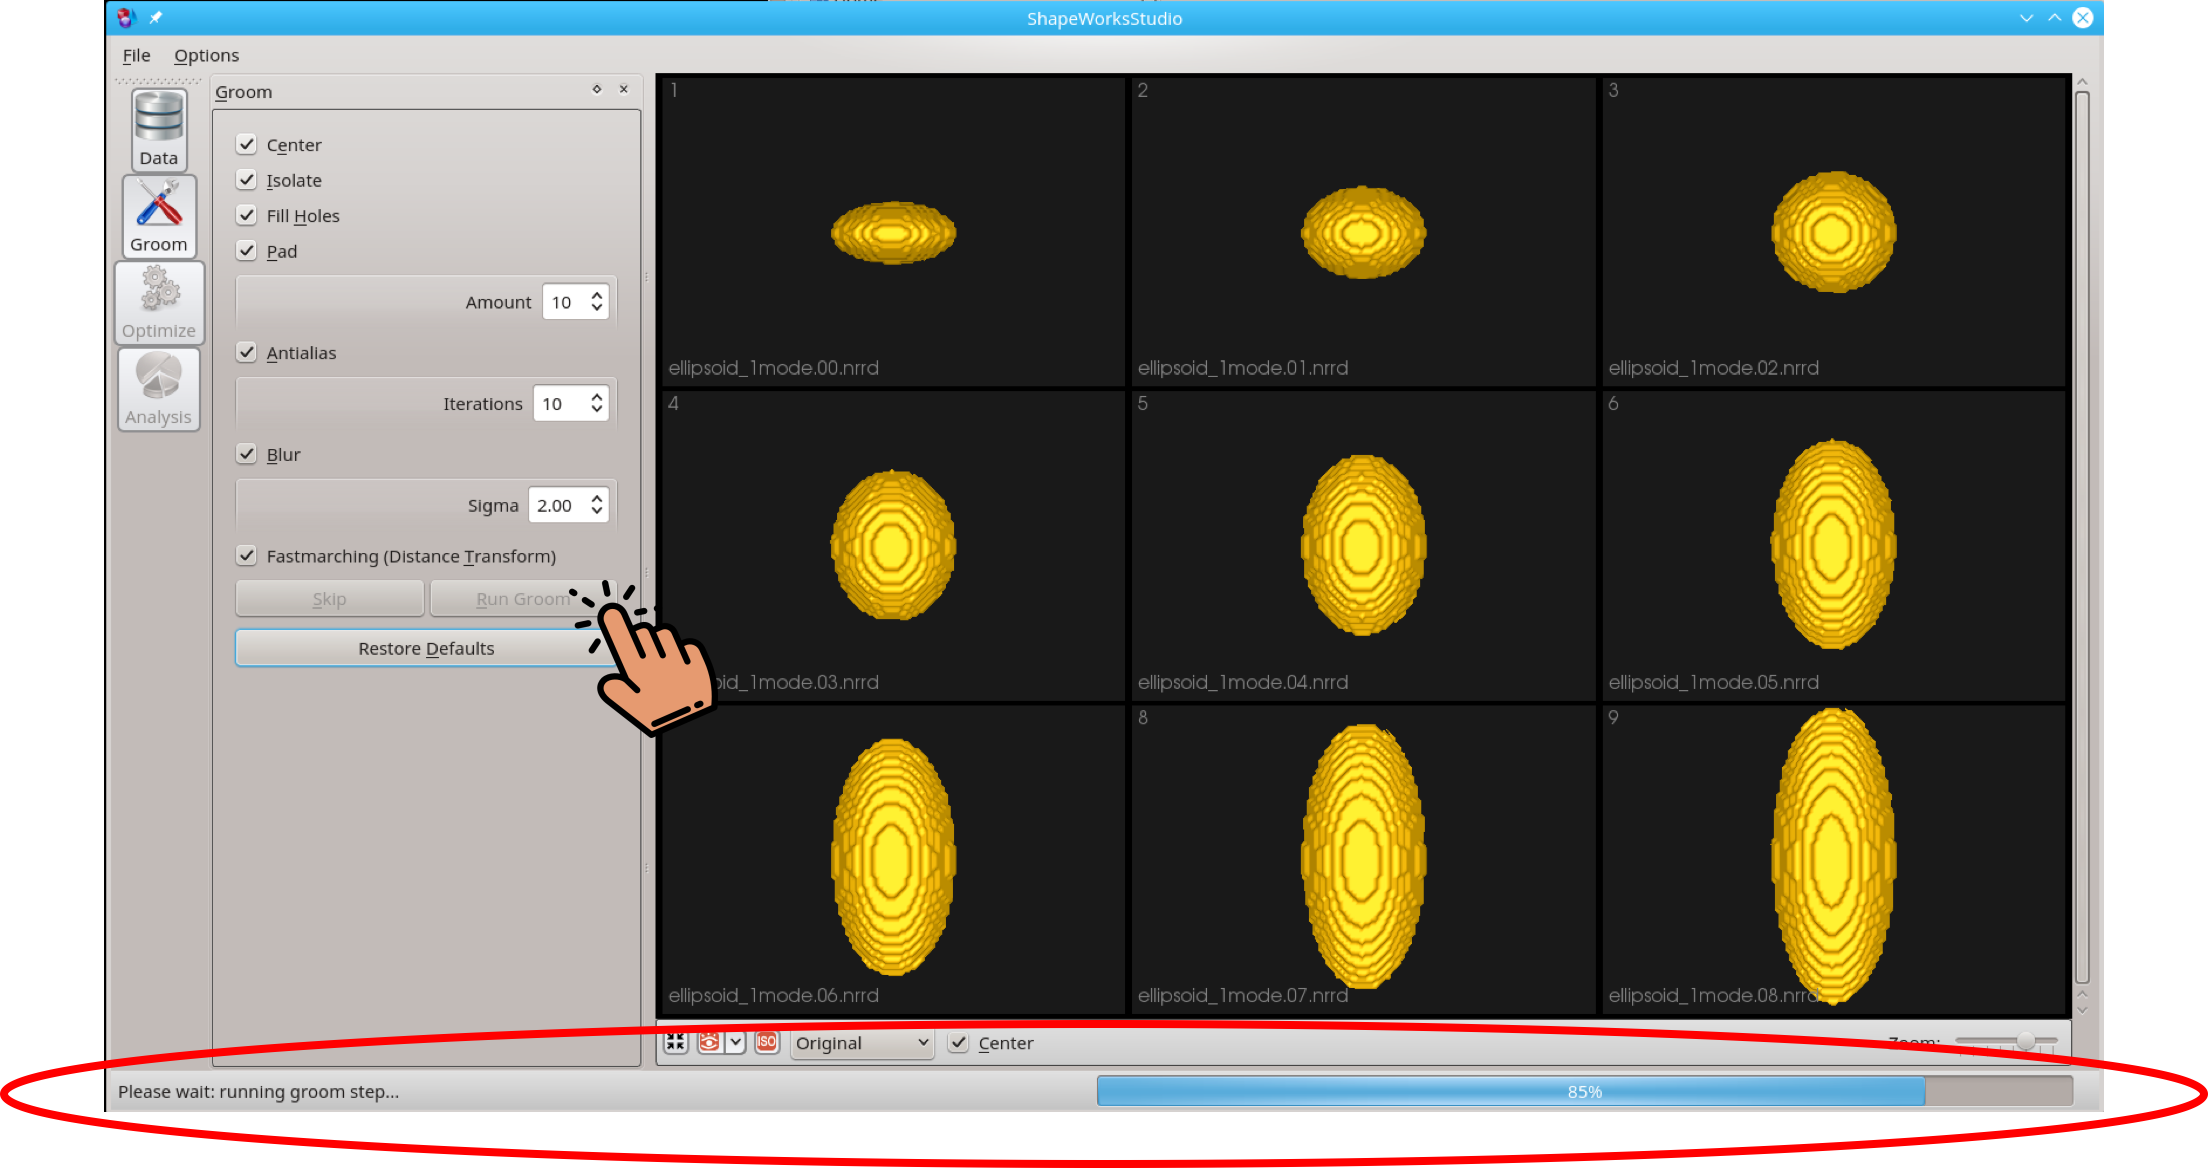
\includegraphics[width=0.9\textwidth]{figs_v2/grooming.png}
	\caption{Grooming shapes in progress }
	\label{fig:grooming}
\end{figure}

\begin{figure}[!htp]
	\centering
	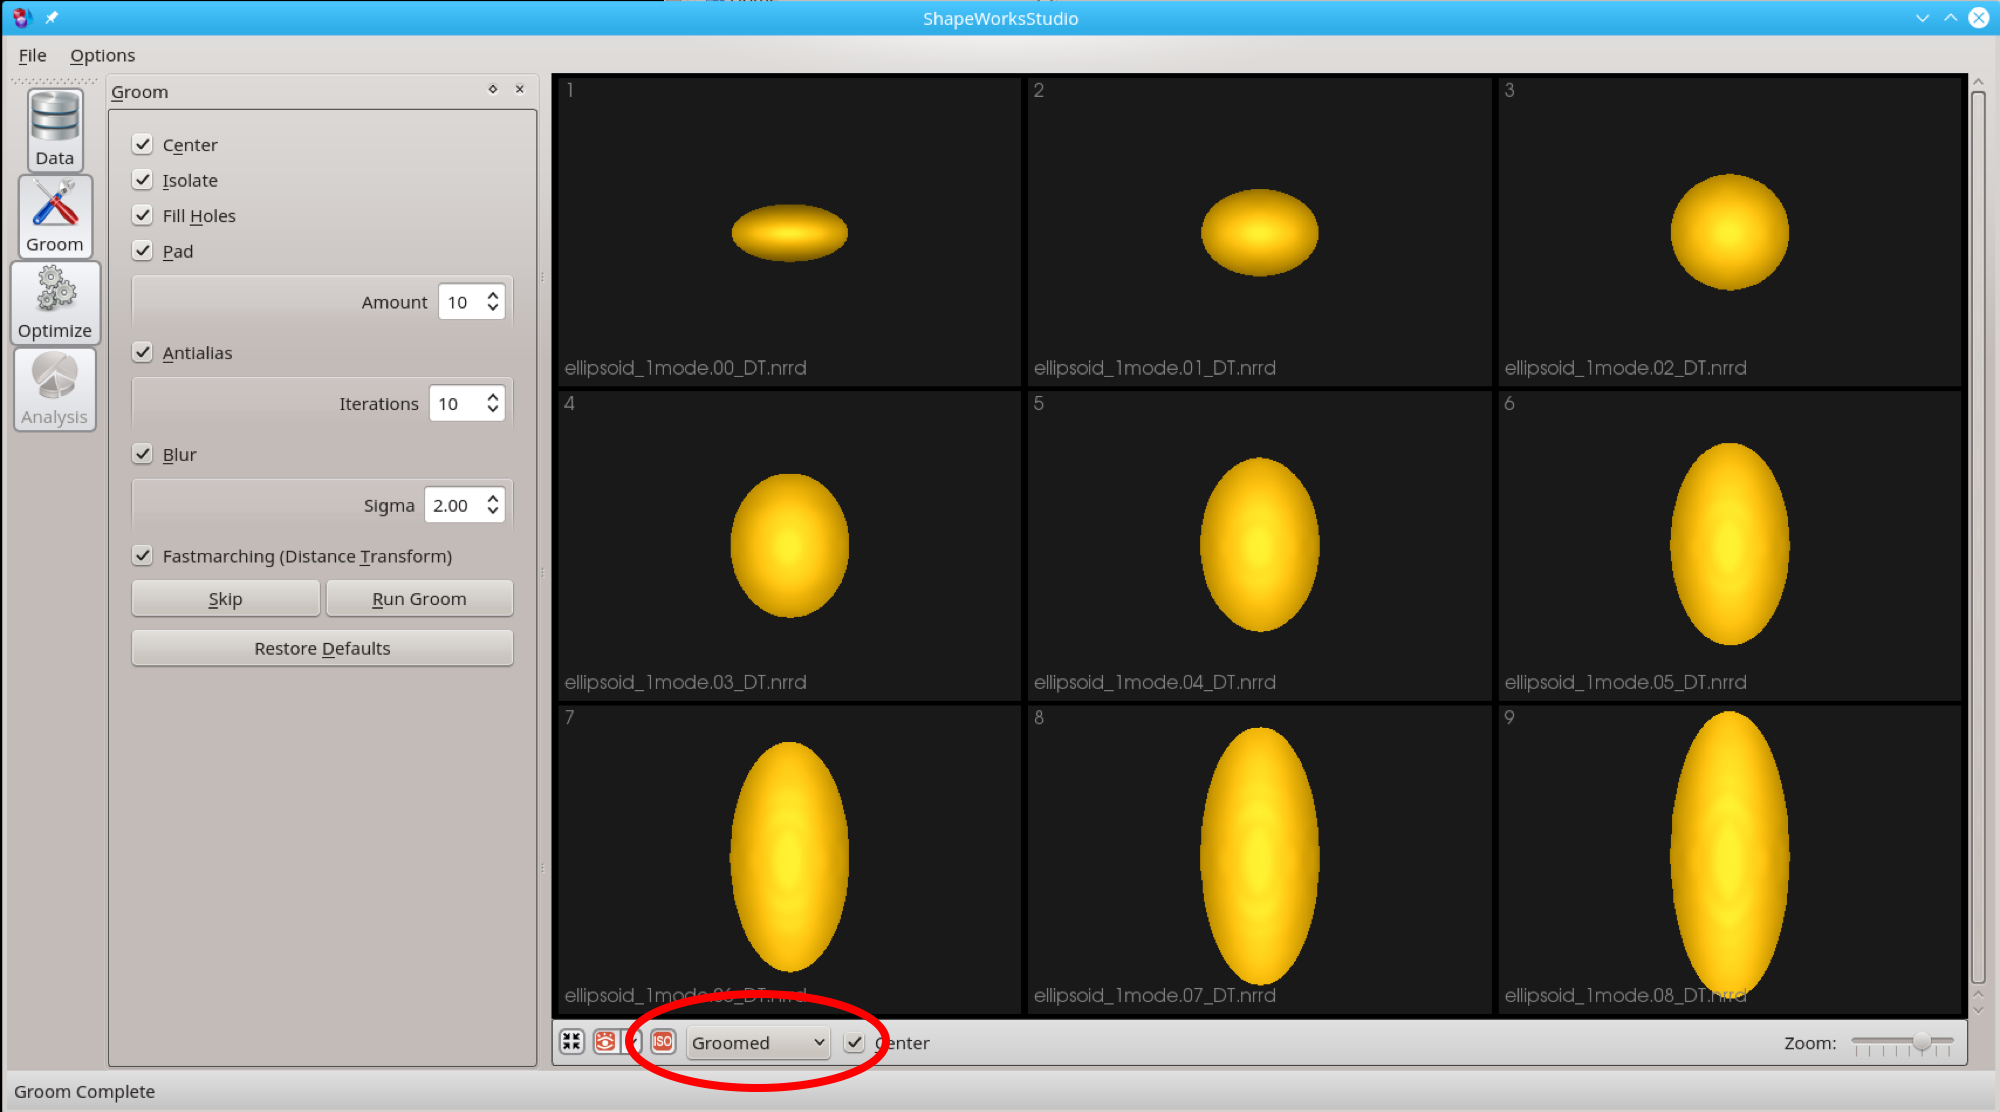
\includegraphics[width=0.9\textwidth]{figs_v2/groomed.png}
	\caption{Groomed shapes, refer to the viewing options to switch between original and groomed shapes}
	\label{fig:groomed}
\end{figure}

\begin{figure}[!htp]
	\centering
	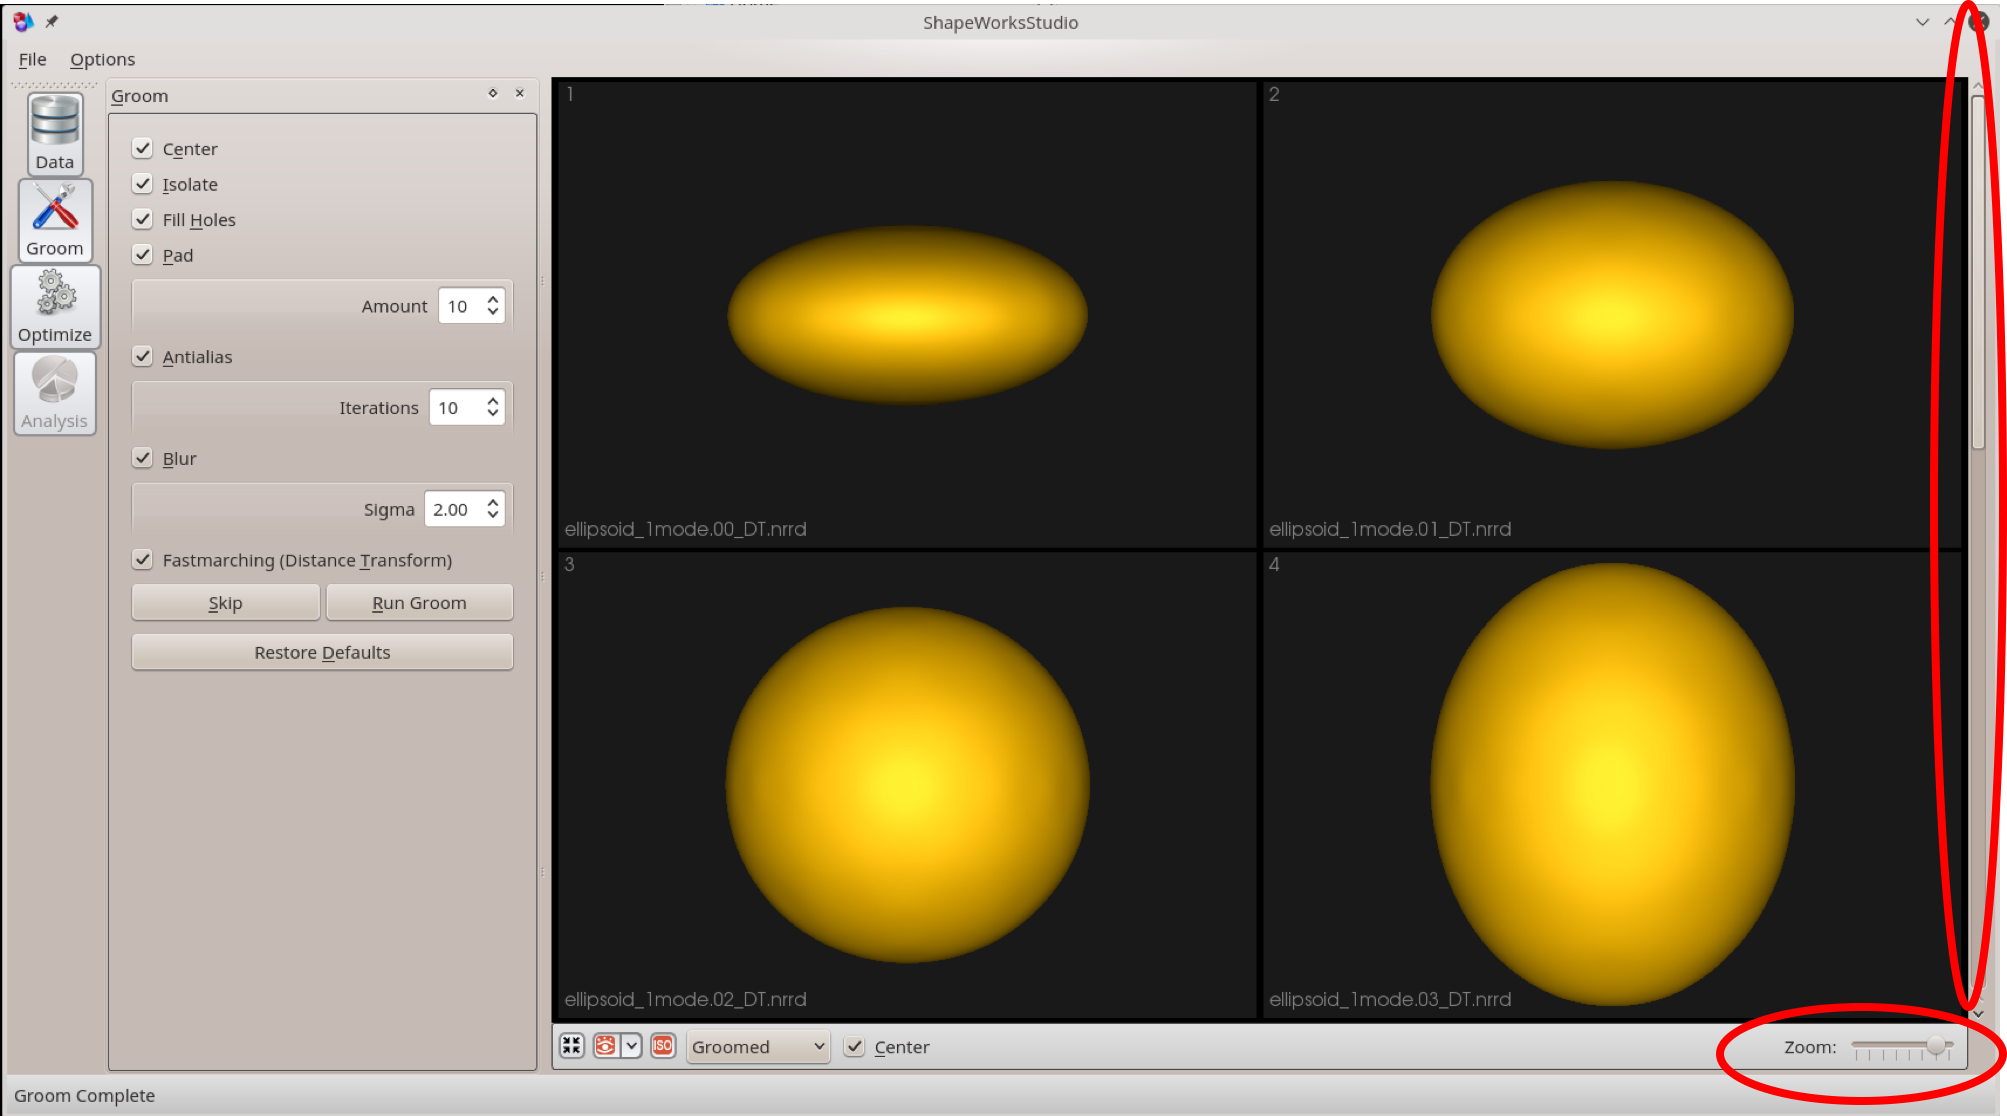
\includegraphics[width=0.9\textwidth]{figs_v2/zoom.png}
	\caption{Use the \texttt{Zoom} slide bar to zoom in/out to display less or more number of shapes. Use the slide bar to move down/up in case of showing a small number of shapes. Right-click and drag to zoom-in and zoom-out individual shapes.}
	\label{fig:zoom}
\end{figure}

\vspace{0.1in}
Fig. \ref{fig:groomed} shows the resulting groomed shapes for a torus ensemble. Note that you can use the drop-down menu from the viewing options bar at the bottom to switch between the original and the groomed shapes. You can also use the \texttt{Zoom} slide bar to display less or more shapes in the rendering window grid and thus see more or less details for individual shapes (see Fig. \ref{fig:zoom}).

\begin{figure}[!htp]
	\begin{minipage}[c]{0.5\textwidth}
		\centering
		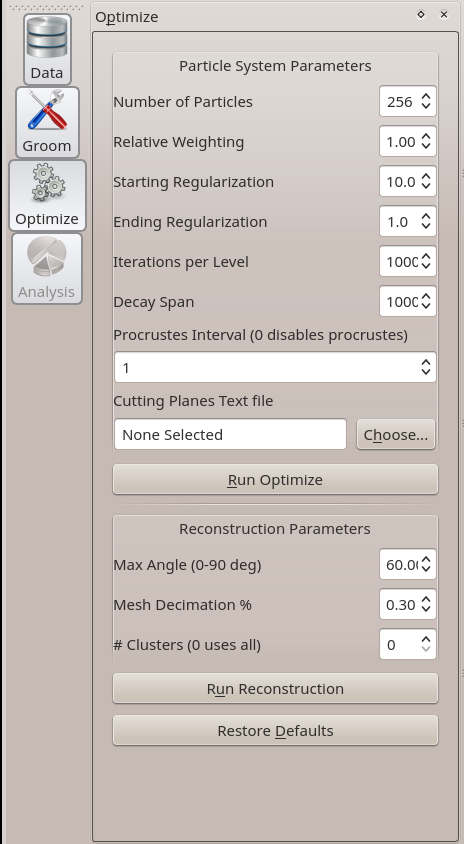
\includegraphics[width=0.7\textwidth]{figs_v2/optimize.png}
	\end{minipage}\hfill
	\begin{minipage}[t]{0.5\textwidth}
		\centering
		\caption{\texttt{Optimize} involves uniformly spreading corresponding particles over the isosurfaces of the groomed shapes. You can control this process by setting the parameters shown } 
		\label{fig:optimize}
	\end{minipage}
\end{figure}


\begin{figure}[!htp]
	\centering
	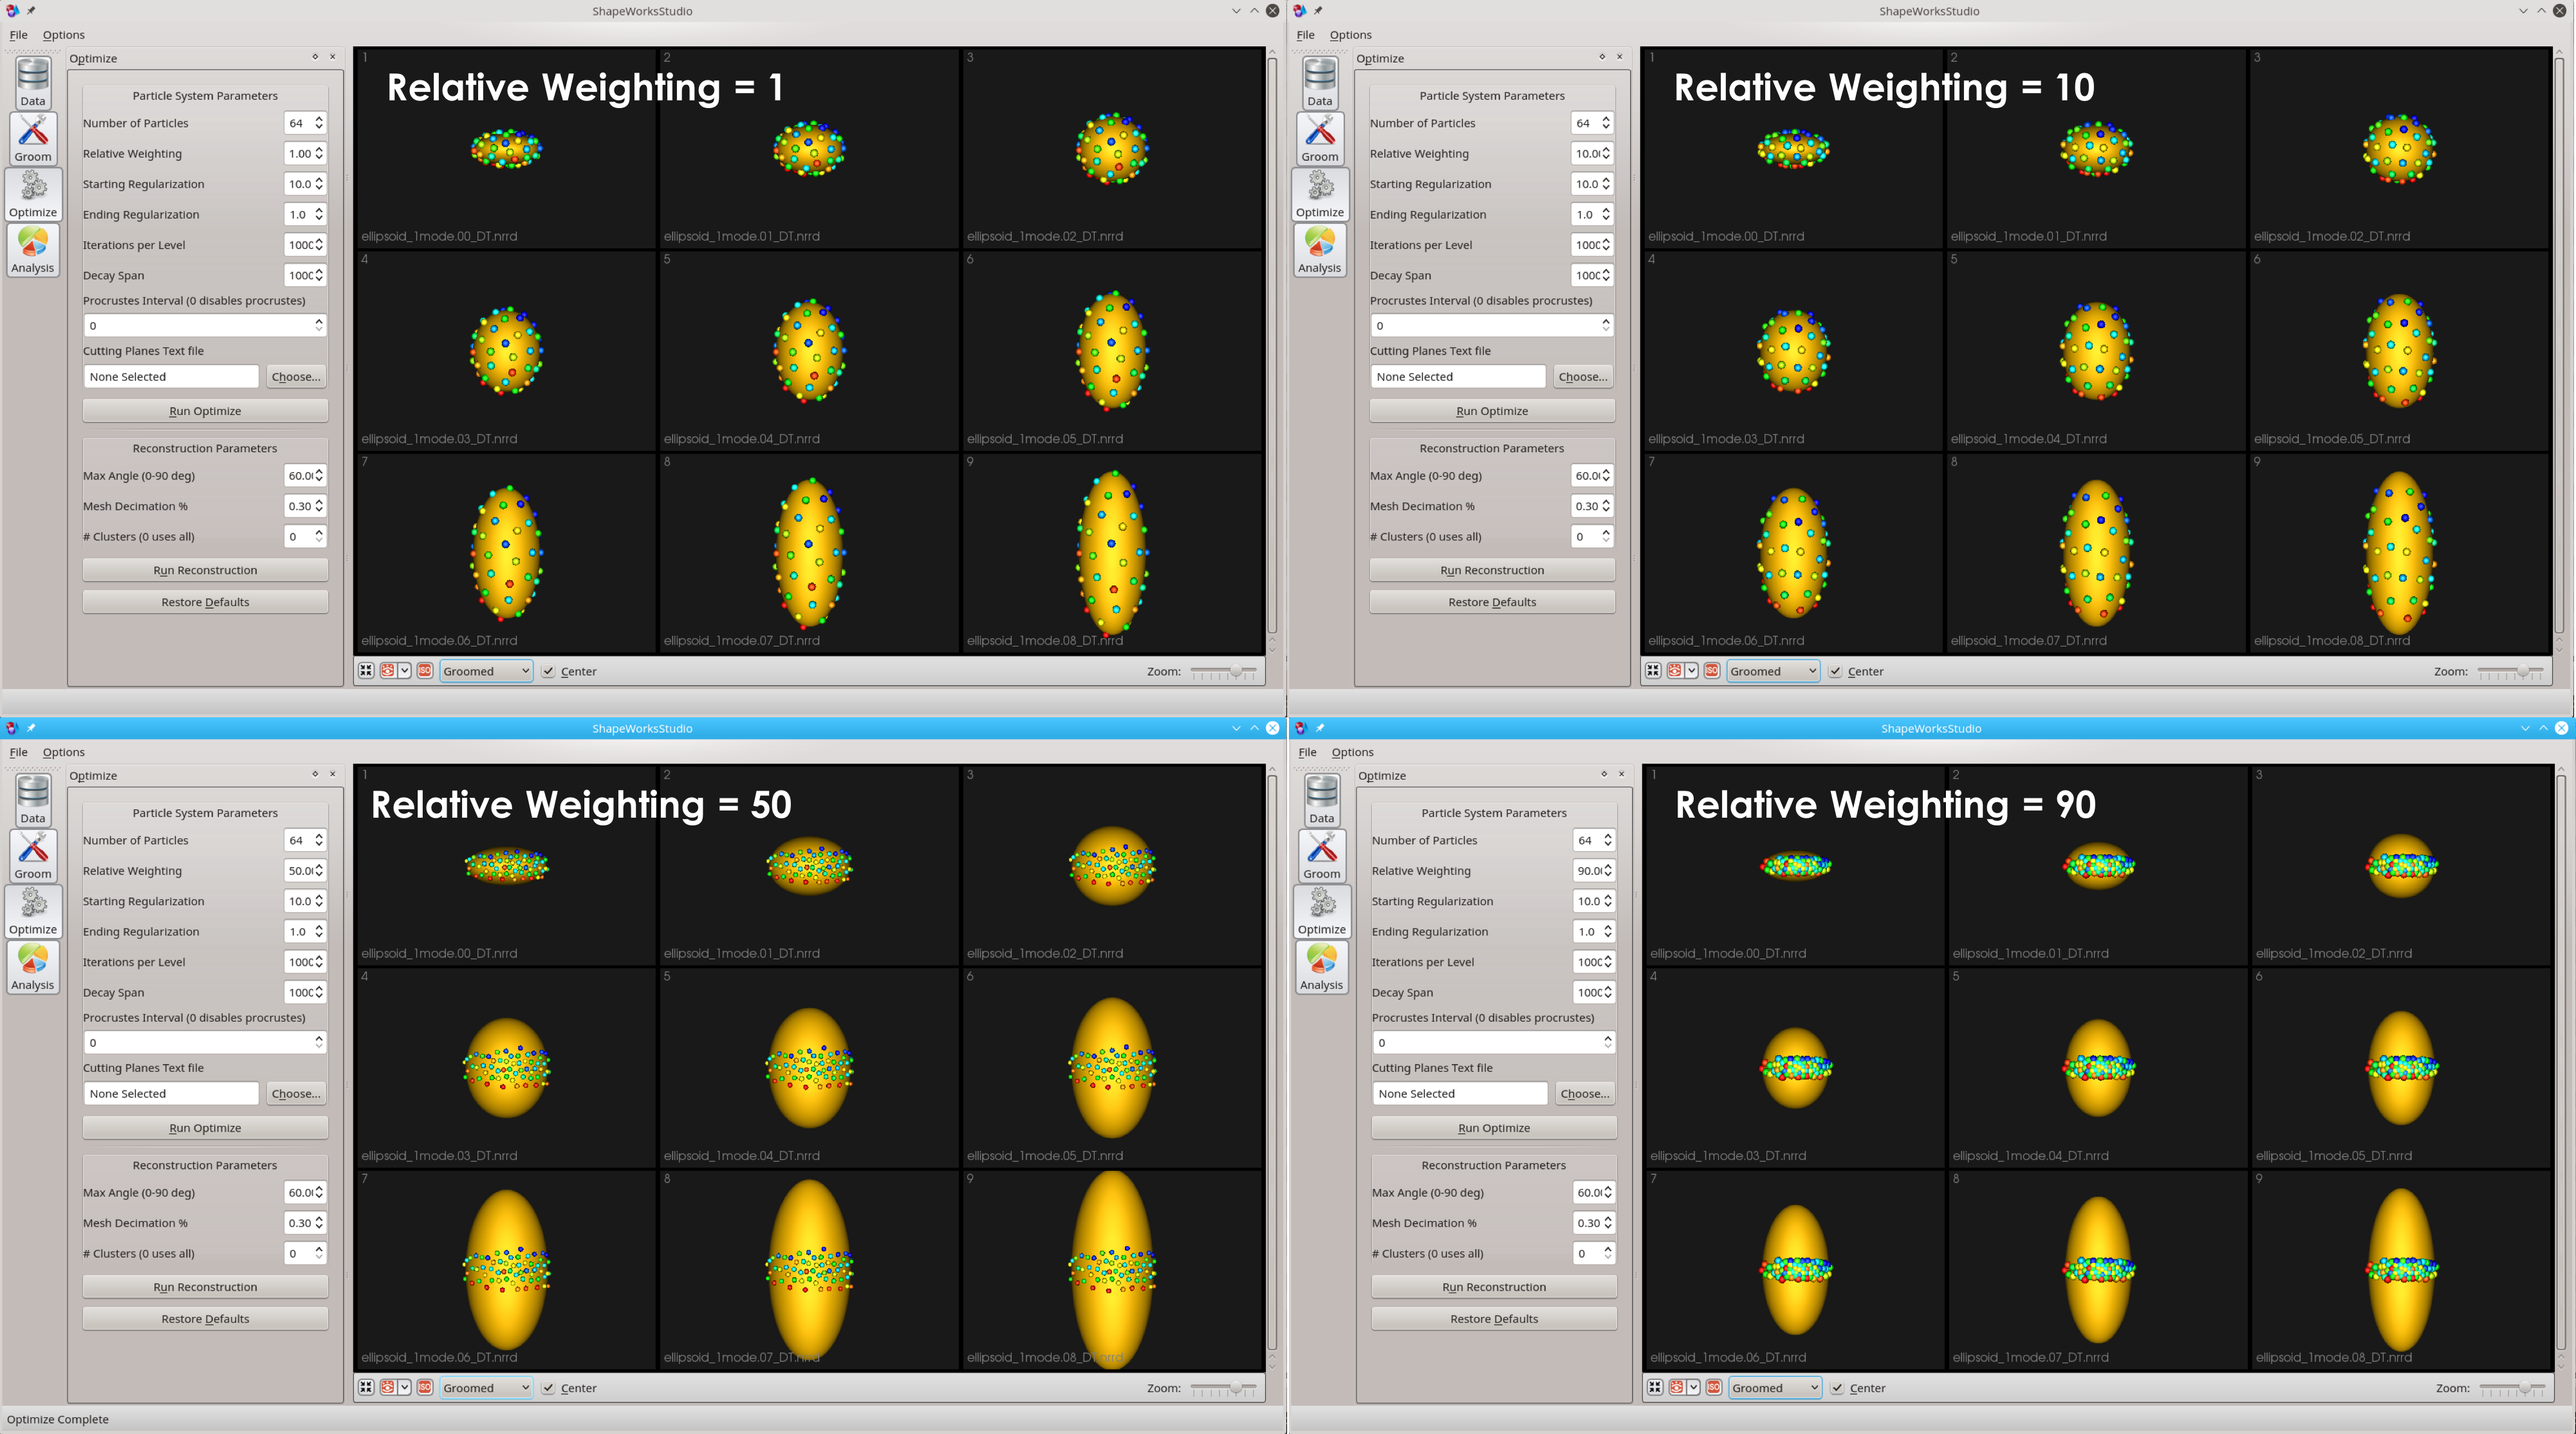
\includegraphics[width=1\textwidth]{figs_v2/ellipsoid_relative_weighting.png}
	\caption{Optimized correspondence model using different relative weightings}
	\label{fig:ellipsoid_relative_weighting}
\end{figure}

\subsection{Optimize}

\noindent\textbf{Correspondence optimization:} Once the grooming step is complete, you can run the optimize step which involves uniformly spreading corresponding particles over the isosurfaces of the groomed shapes. You can control the optimization process via tuning the following parameters (see Fig. \ref{fig:optimize}):

\begin{itemize}
	\item[-] \textbf{Number of Particles:} Specifies the number of particles to be used to represent each shape in the ensemble. Keep in mind that the actual particle count will be a power of two greater than the provided number.

	\item[-] \textbf{Relative Weighting:} This is the value of parameter "alpha" from the energy equation $Q =  \alpha H(\mathbf{Z}) -  \sum_k H(\mathbf{x}_k)$. This parameters weights the correspondence part of the objective function with higher values giving more importance to the correspondence entropy and lower values guide the optimization towards better surface sampling. Recommended value is $1$, yet for some ensembles, one might tune this parameter to balance the trade-off between surface sampling and particle correspondence. Fig. \ref{fig:ellipsoid_relative_weighting} shows the optimized correspondence models using different relative weighting values. It can be noted that with allowing correspondence to dominate the optimization process (using higher relative weighting), particles tend to be distributed in regions with relatively small variability across the given population. As the relative weighting tends to infinity, particles will be cluttered in one spot on each surface which means that all shapes will be represented as a point at the shape space origin. Figs \ref{fig:rel_low_hover1}-\ref{fig:rel_high_hover2} show visual correspondence inspection where it can be observed that when using lower relative weighting, i.e., allowing surface sampling to dominate the optimization process, resulting particles become out-of-correspondence.

\item[-] \textbf{Starting/Ending Regularization:}  This option determines the regularization on the covariance matrix for the shape-space entropy estimation. This regularization exponentially decays along optimization iterations where better covariance structure can be estimated with better correspondence model. Higher regularization values would undermine the underlying covariance structure of the ensemble and favors all shapes to converge to the mean shape. Hence it is recommended to use starting regularization value as $\approx 5\%$ of the expected highest eigenvalue of the covariance matrix while ending regularization can be taken as ten times less than the starting value. 

\item[-] \textbf{Iterations per Level:} Specifies the number of iterations to run between successive particle splits during an initialization phase. This allows the particle system at a given granularity to converge to a stable state before more particles are added.

\end{itemize}

\begin{figure}[!htp]
	\centering
	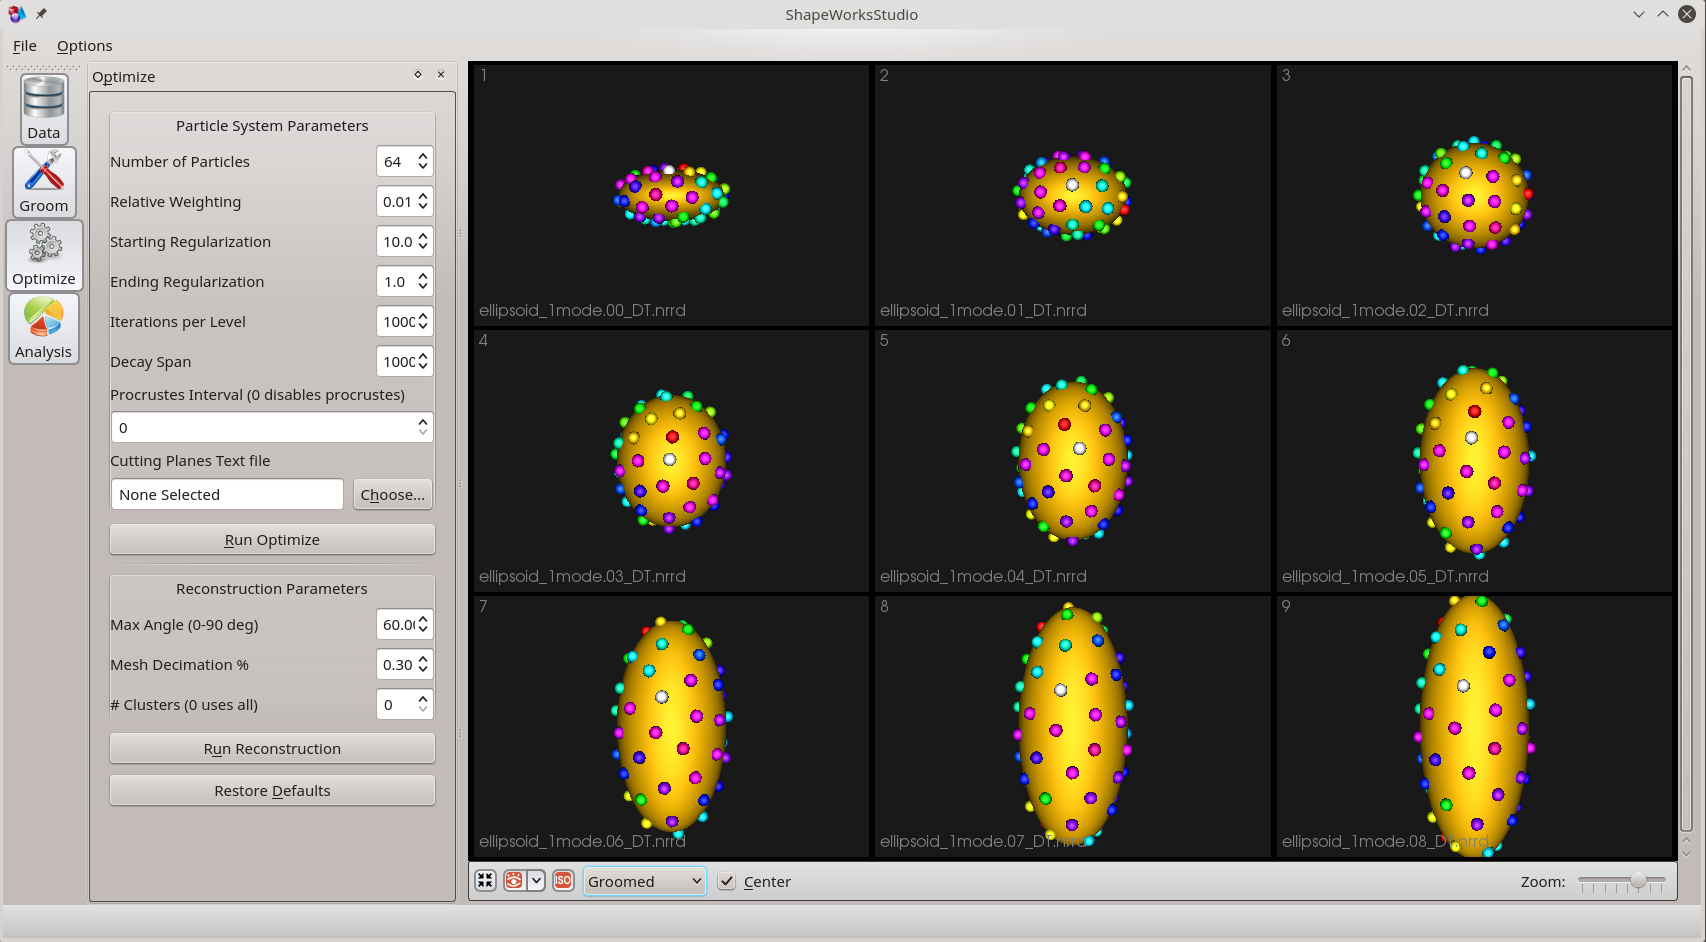
\includegraphics[width=0.82\textwidth]{figs_v2/ellipsoid_w001_corr_qc_1.png}
	\caption{Optimized correspondence model using relative weighting $ = 0.01$ with one particle selected to visualize correspondence. Simply hover on the required particle and press 1, the particle will be colored in white and all other particles will be colored based on its distance to the selected particle. To recover the original display, type 1 or 2 while NOT hovering over any particles}
	\label{fig:rel_low_hover1}
\end{figure}

\begin{figure}[!htp]
	\centering
	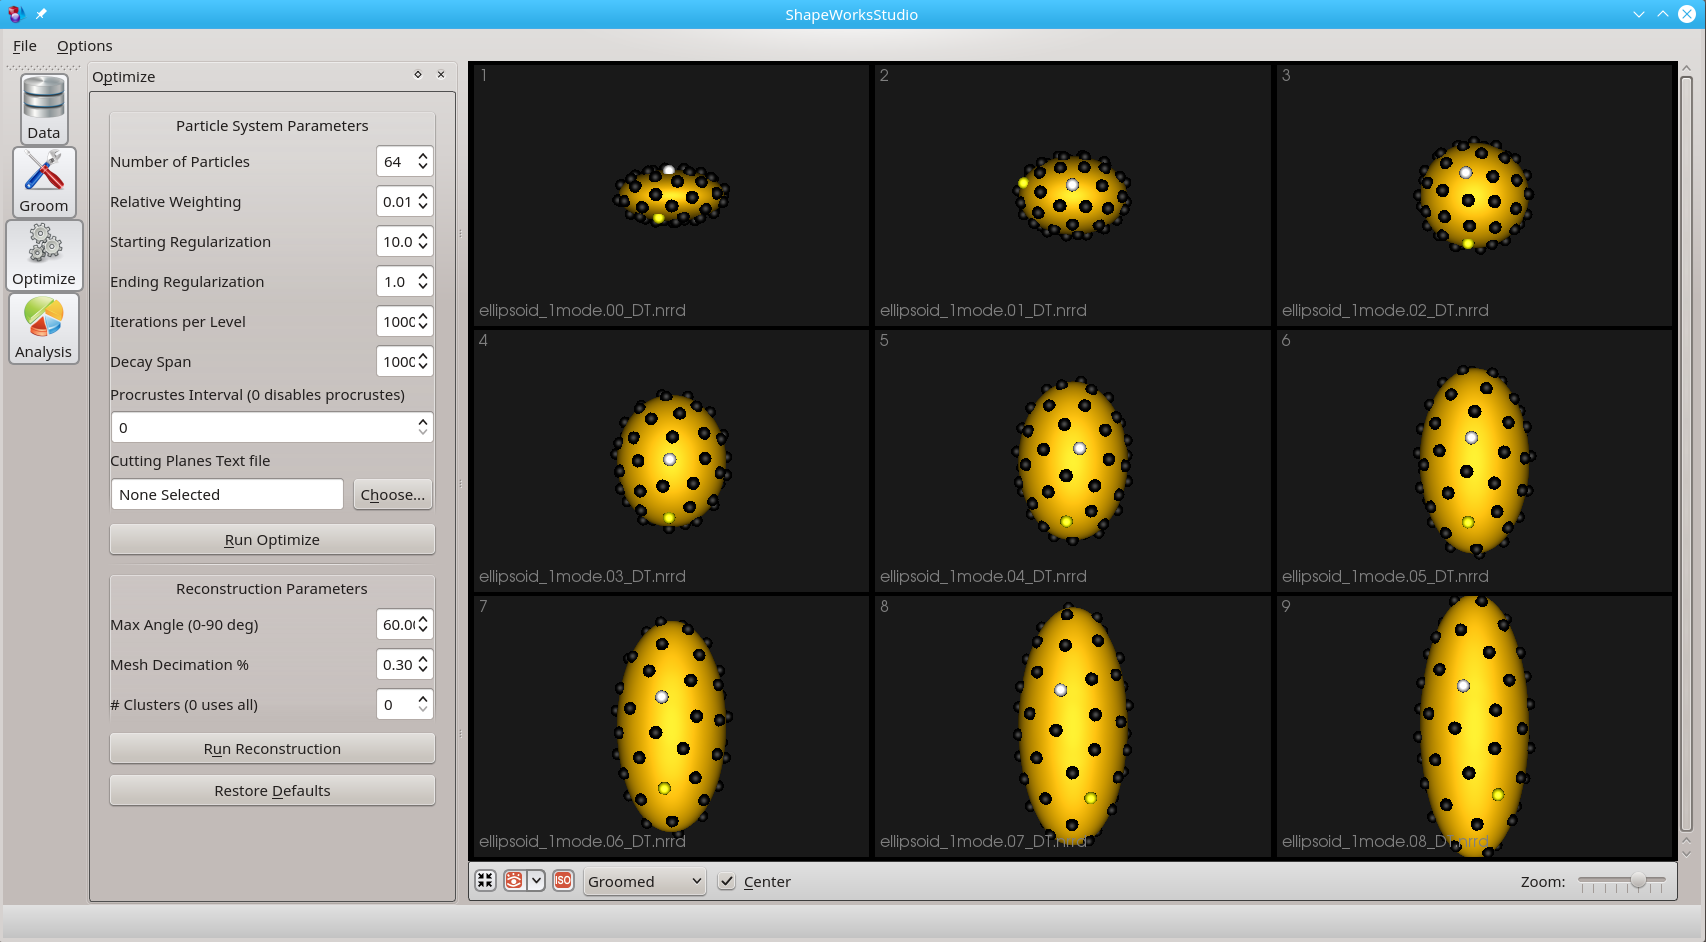
\includegraphics[width=0.82\textwidth]{figs_v2/ellipsoid_w001_corr_qc_2.png}
	\caption{Optimized correspondence model using relative weighting $ = 0.01$ with two particles selected to visualize pairwise correspondence. Simply hover on the second required particle and press 2, the second particle will be colored in yellow and all other particles will be colored in black. To recover the original display, type 1 or 2 while NOT hovering over any particles}
	\label{fig:rel_low_hover2}
\end{figure}

\begin{figure}[!htp]
	\centering
	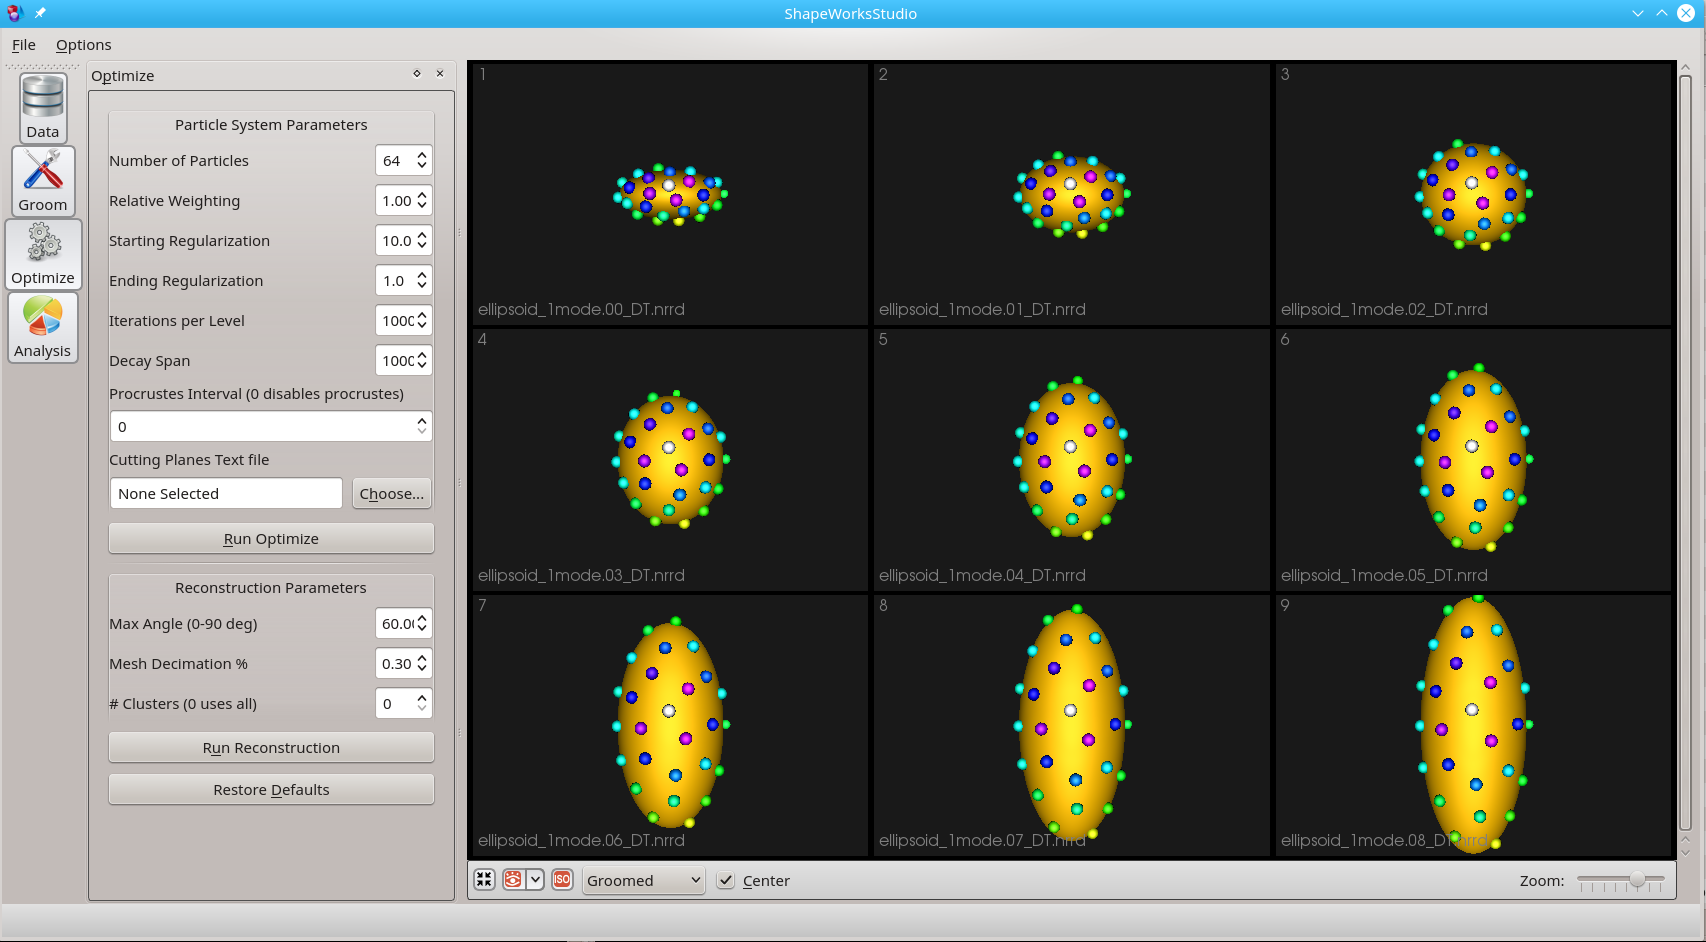
\includegraphics[width=0.82\textwidth]{figs_v2/ellipsoid_w1_corr_qc_1.png}
	\caption{Optimized correspondence model using relative weighting $ = 1$ with one particle selected to visualize correspondence. Simply hover on the required particle and press 1, the particle will be colored in white and all other particles will be colored based on its distance to the selected particle. . To recover the original display, type 1 or 2 while NOT hovering over any particles. Note that particles are out-of-correspondence since surface sampling is dominating the optimization process}
	\label{fig:rel_high_hover1}
\end{figure}

\begin{figure}[!htp]
	\centering
	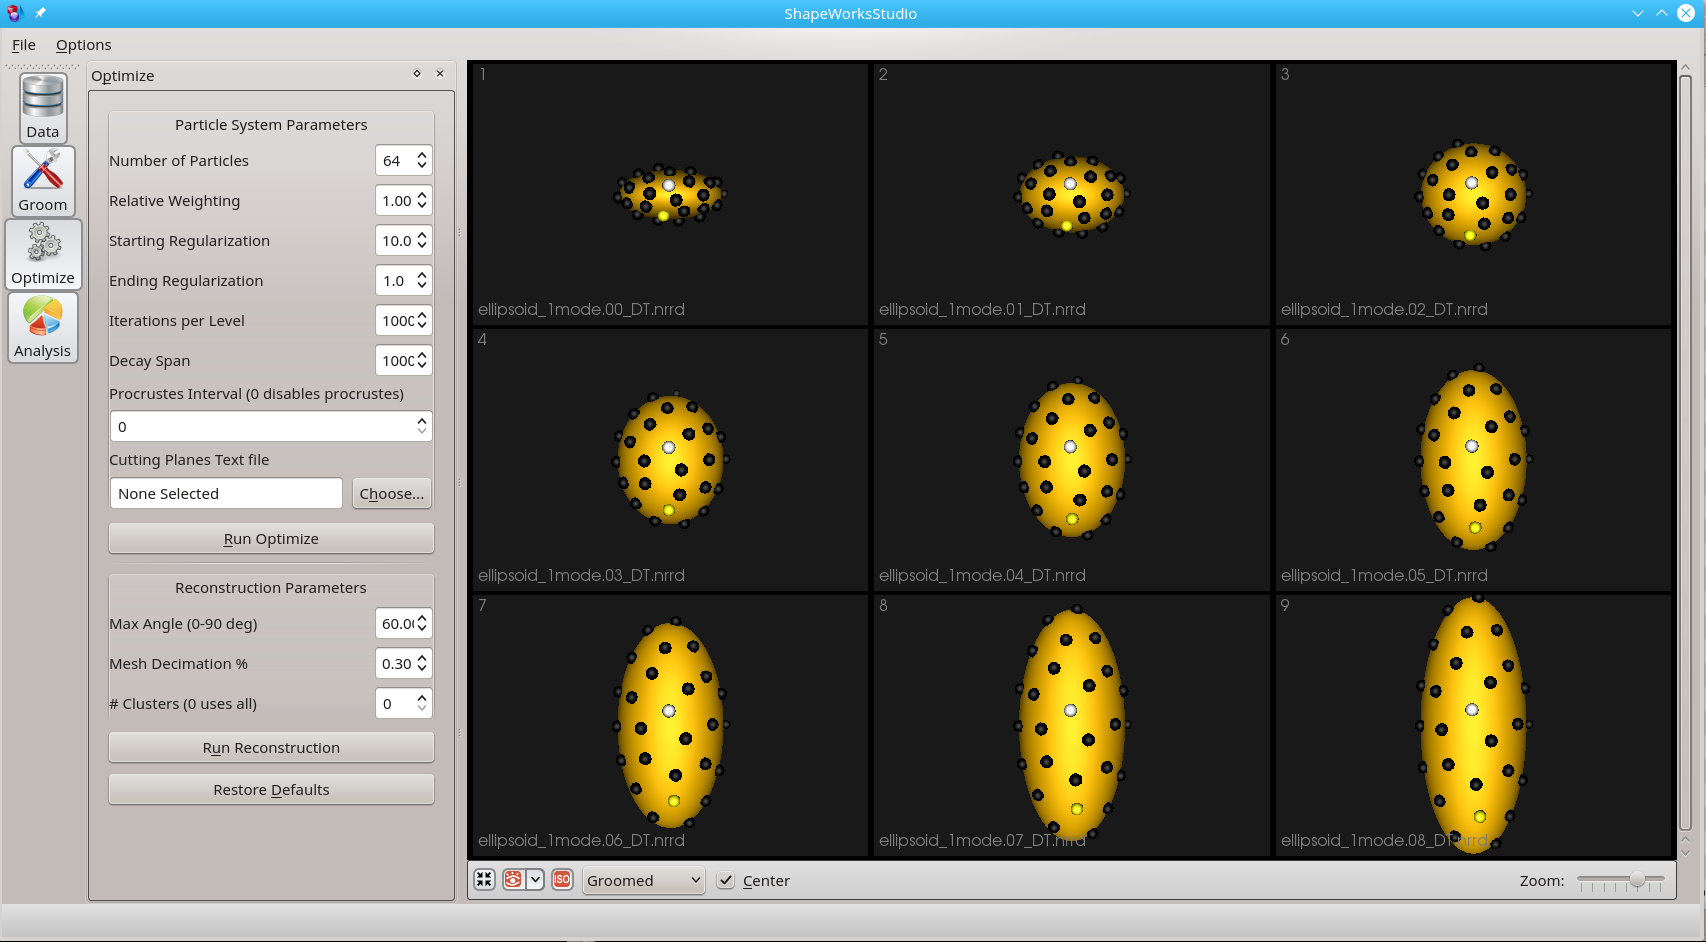
\includegraphics[width=0.82\textwidth]{figs_v2/ellipsoid_w1_corr_qc_2.png}
	\caption{Optimized correspondence model using relative weighting $ = 1$ with two particles selected to visualize pairwise correspondence. Simply hover on the second required particle and press 2, the second particle will be colored in yellow and all other particles will be colored in black. . To recover the original display, type 1 or 2 while NOT hovering over any particles. Note that particles are out-of-correspondence since surface sampling is dominating the optimization process}
	\label{fig:rel_high_hover2}
\end{figure}

\begin{itemize}

\item[-] \textbf{Decay Span:} The parameters Starting Regularization, Ending Regularization, and Decay Span define an “annealing” type optimization, where the minimum variance starts at Starting Regularization and exponentially decreases over Decay Span to the
Ending Regularization value. This is usually the same number as iterations.

\item[-] \textbf{Run Optimize:} Click this when you are ready for optimizing. This step takes a while. A progress indicator shows the tool is working. The timing of this step depends primarily on number of shapes, number of particles and number of iterations specified. You can watch the terminal to keep track of intermediate output which is also written to ShapeWorksStudioTools.log file next to the executable. Upon completion, the rendering working will show the optimized correspondence model, i.e. particles, overlayed onto their groomed surfaces.

\item[-] \textbf{Procrustes Interval:} This parameter determines how often a procrustes alignment step is performed during the optimization. If set, Studio will do a Procrustes registration based on the current correspondence positions at the specified interval. The registration establishes a different common coordinate frame for correspondences, but preserves the local coordinate frames for each shape sample. If your data is pre-aligned, it is recommended to use disable this alignment by setting the interval to zero.

\item[-] \textbf{Cutting Planes Text file:} To handle open surfaces, you can use cutting planes to limit particle distribution. A cutting plane is defined  using the local coordinates of three points the lie on that plane. You can use a different cutting plane per shape sample (i.e., image volume) or a single cutting plane for all samples. Cutting planes are stored in plain text files. These files contain no header, and are simply a list of the three point positions for each plane written as follows 

 \noindent\texttt{ax1 ay1 az1 bx1 by1 bz1 cx1 cy1 cz1}\\
 \noindent\texttt{ax2 ay2 az2 bx2 by2 bz2 cx2 cy2 cz2}\\
 ... \\
 \noindent\texttt{axN ayN azN bxN byN bzN cxN cyN czN}\\
 \noindent where \texttt{x y z} are floating point numbers, \texttt{a,b,c} refers to the three points that define a plane and \texttt{N} is the number of shape samples. In case of a single cutting plane for all shapes, the text file may contain the three plane points repeated N-times or a single line containing the three points. 

\end{itemize}

\noindent\textbf{Particle-based surface reconstruction:}  Studio supports a particle-based shape reconstruction to enhance the visualization of population-/sample-level shape models and provide denser correspondences among the input shapes with a smaller number of particles. This step implements an unbiased framework for template/mean mesh construction that involves warping/deforming samples' distance transforms to the mean space to compute a mean distance transform. The template dense mesh is then be constructed by triangulating the isosurface of this mean distance transform using a mix of VTK-based isosurfacing and Preview-based\footnote{\texttt{https://febio.org/preview/}} mesh quality control. To recover a sample-specific surface mesh, a warping function is then constructed to deform the template dense mesh to the sample space using the sample’s and mean particle systems as control points. For large cohorts with high-resolution image voles, the time for template mesh construction can be intolerable from the end-user perspective. We mitigate this pitfall by performing a shape-based clustering where only a representative set of shapes will contribute to the template mesh computation. The reconstruction step can be controlled using the following set of parameters. \vspace{0.2in}


\begin{figure}[!htp]
	\centering
	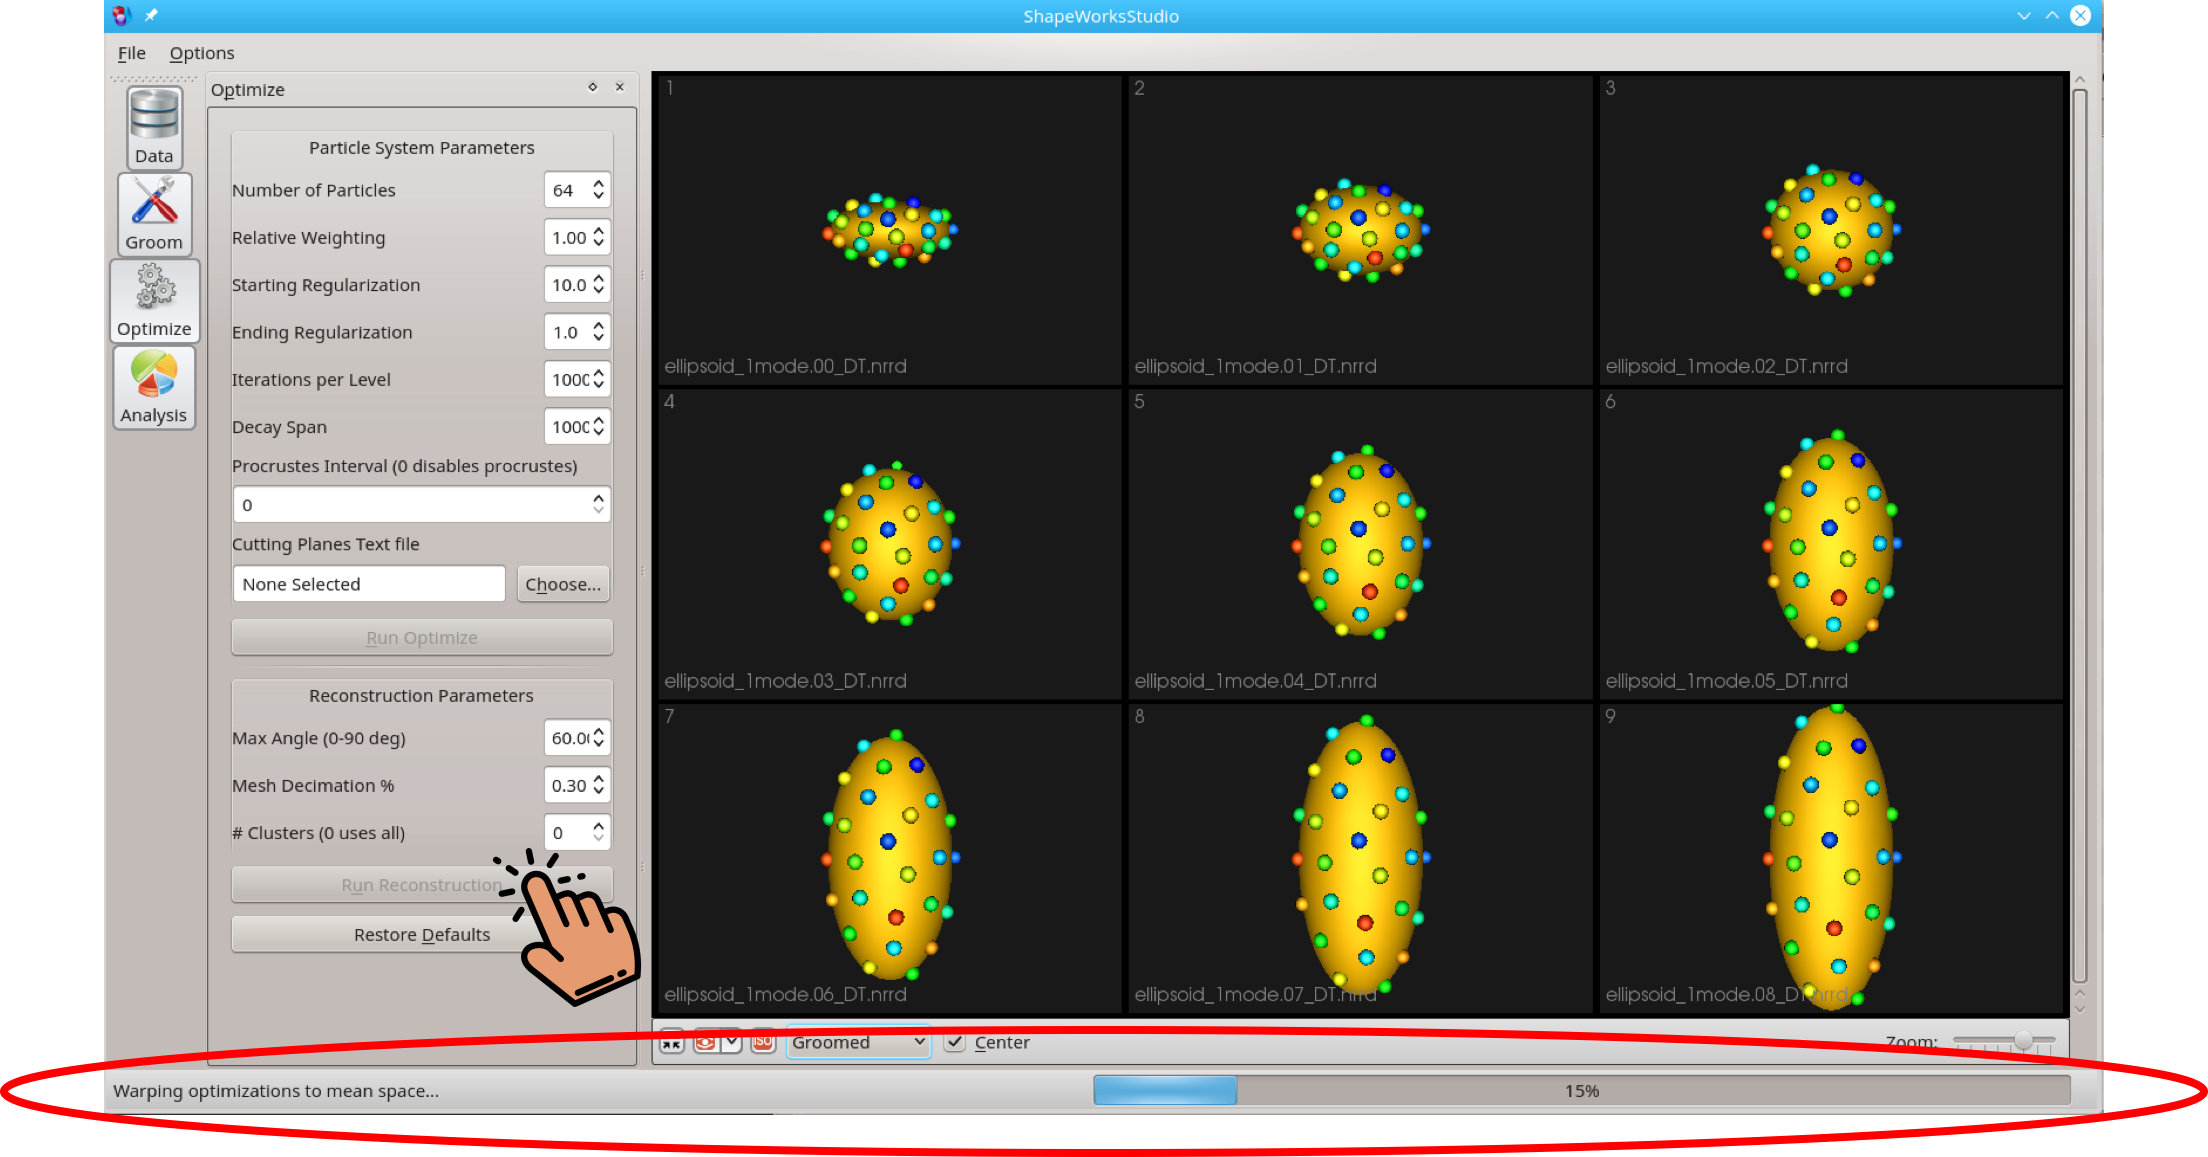
\includegraphics[width=0.82\textwidth]{figs_v2/reconstructing.png}
	\caption{Reconstruction in progress }
	\label{fig:reconstructing}
\end{figure}


\begin{figure}[!htp]
	\centering
	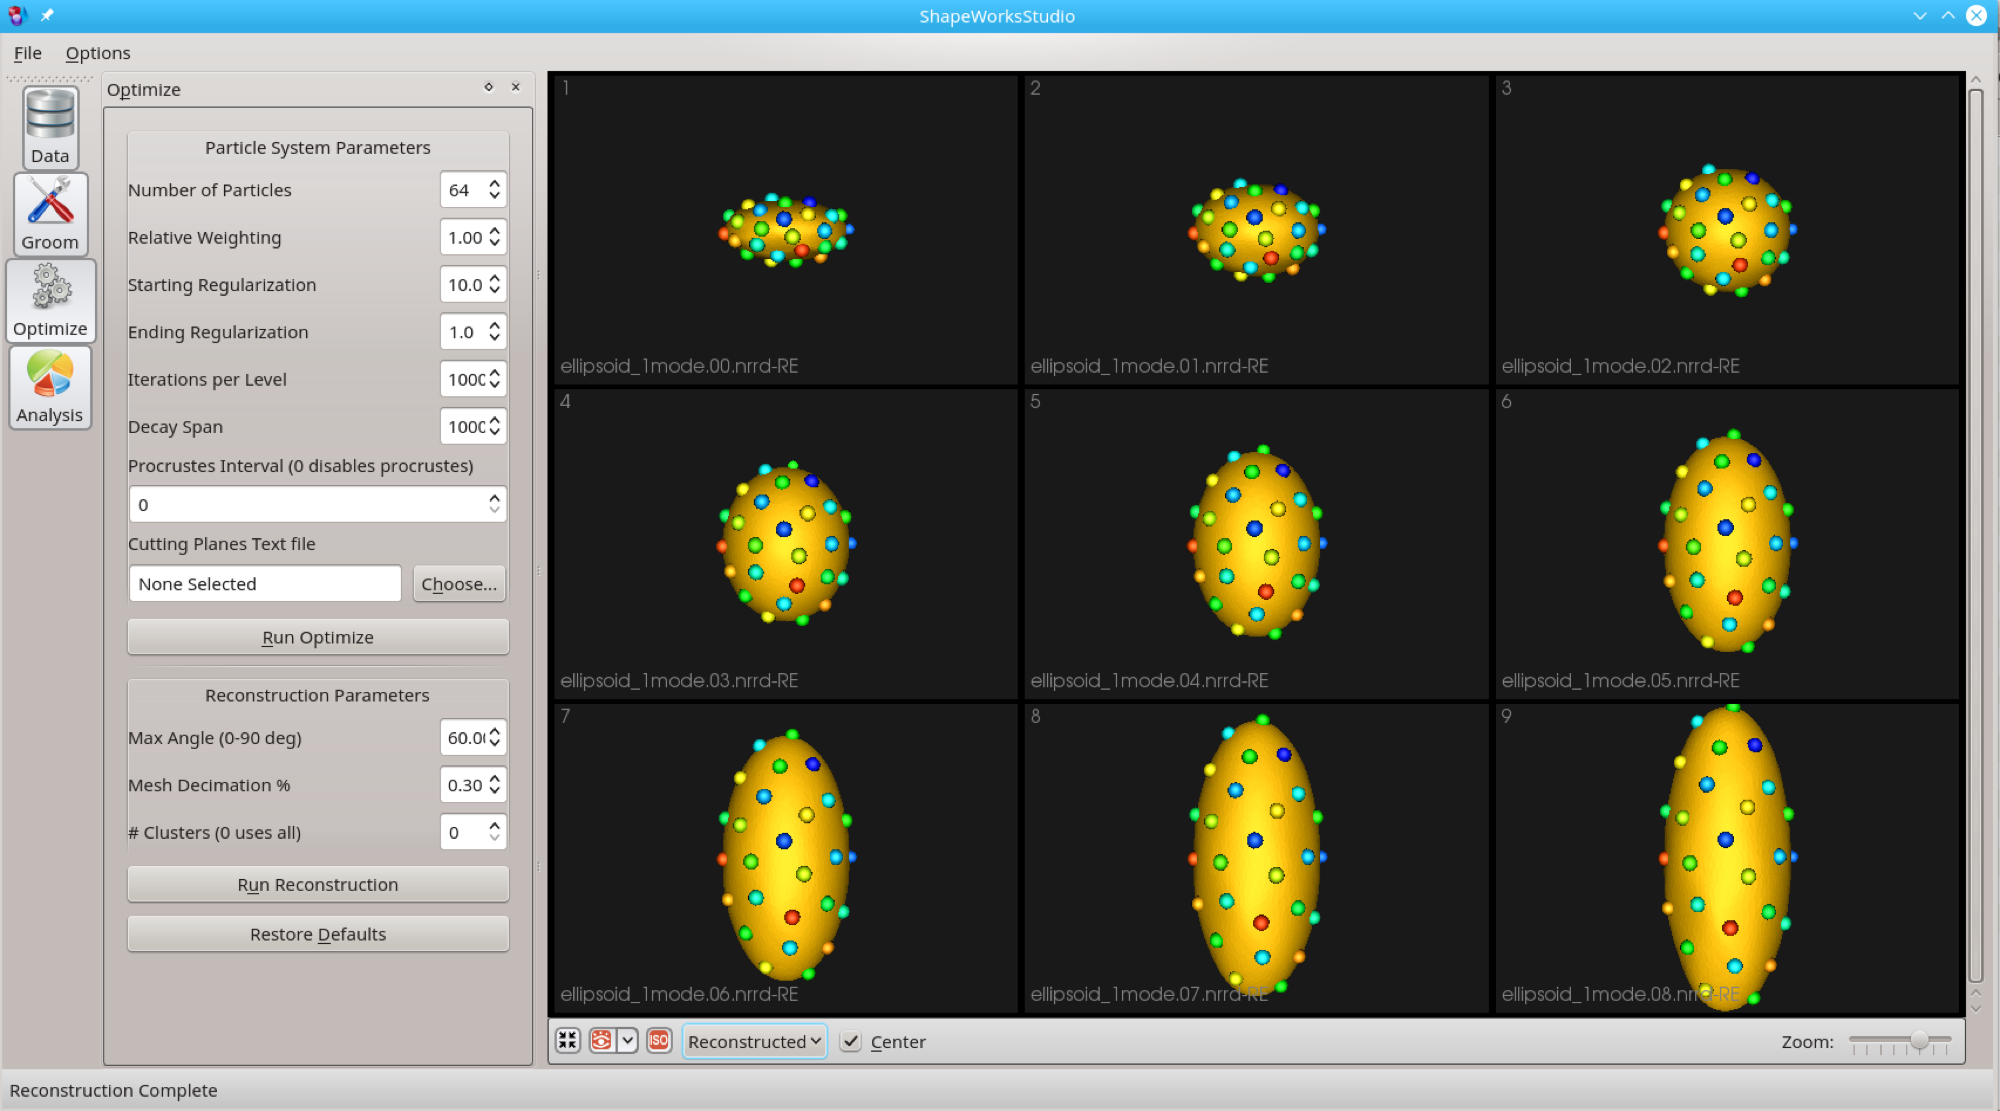
\includegraphics[width=0.82\textwidth]{figs_v2/reconstructed.png}
	\caption{Reconstructed shapes, refer to the viewing options to switch between groomed and reconstructed shapes to quality-control the reconstructed surfaces. Irregular reconstructions are typically attributed to a sub-optimal correspondence model. In this case, you could consider trying out different optimization parameters.}
	\label{fig:reconstructed}
\end{figure}


\begin{itemize}
	\item[-] \textbf{Max Angle:} This is the largent angle between particle normals (from respective samples) permitted to label the particle as a “good” corresponding particle across the given population, and is useful for surface reconstruction.

	\item[-] \textbf{Mesh Decimation:} The “PreView” library code can decimate the number of triangles to the value set here. The default is “0.30” or 30 percent.

	\item[-] \textbf{\# Clusters:}  To help speed up reconstruction, you can define how many samples/clusters are used to warp their image volumed into the mean space. “0” indicates to use all of the samples.

	\item[-] \textbf{Run Reconstruction:}  Click this to run the reconstruction step. If it fails, the isosurface filter from the visualization toolkit (VTK) is used instead to generate the final surface reconstructions. You can re-run with different Optimizations as needed.

	\item[-] \textbf{Restore Defaults:}  Click this to restore all values to their program defaults.
\end{itemize}


\begin{wrapfigure}{r}{0.33\textwidth}
	\centering
	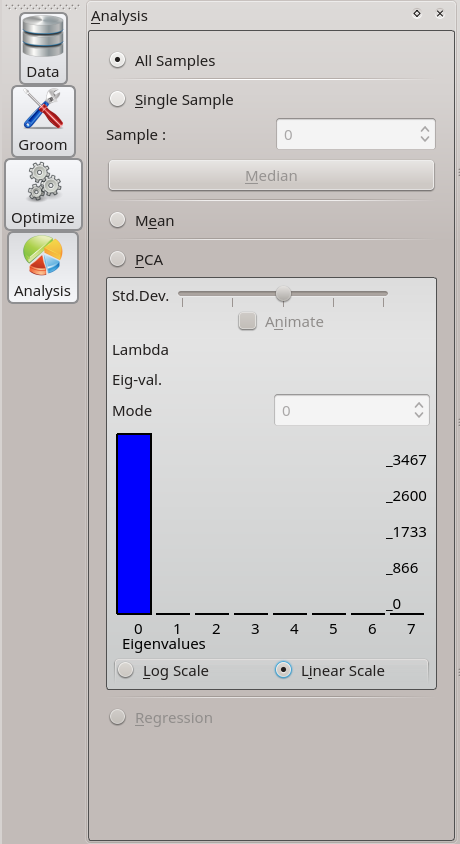
\includegraphics[width=0.33\textwidth]{figs_v2/analysis.png}
	\caption{Analysis step}
	\label{fig:analysis}
\end{wrapfigure}%\clearpage


\subsection{Analysis}

The analysis step can be used to visualize optimized correspondence positions, along with surface reconstructions based on the correspondences. It also computes a principal component analysis (PCA) of the correspondences, and allows you to visualize the variation in each of the modes of the PCA. The mean shapes and the median shapes can be reconstructed. %, and ShapeWorksView allows you to assign group labels to your samples, in order to visualize the differences in mean shape between the groups.
The following options are available (see Fig. \ref{fig:analysis}):

\begin{itemize}
\item[-] \textbf{All Samples:} Display all of the shape samples along with the correspondence model (i.e. corresponding particles if optimzed) on the screen.
\item[-] \textbf{Single Sample:} Display only one sample. You can select a particular number, or click "median" to display the shape that is the computed median of all the shapes.
\item[-] \textbf{Mean:} Display the computed mean of the shapes based on the optimized correspondence model.
\end{itemize}

\clearpage


\begin{figure}[!htp]
	\centering
	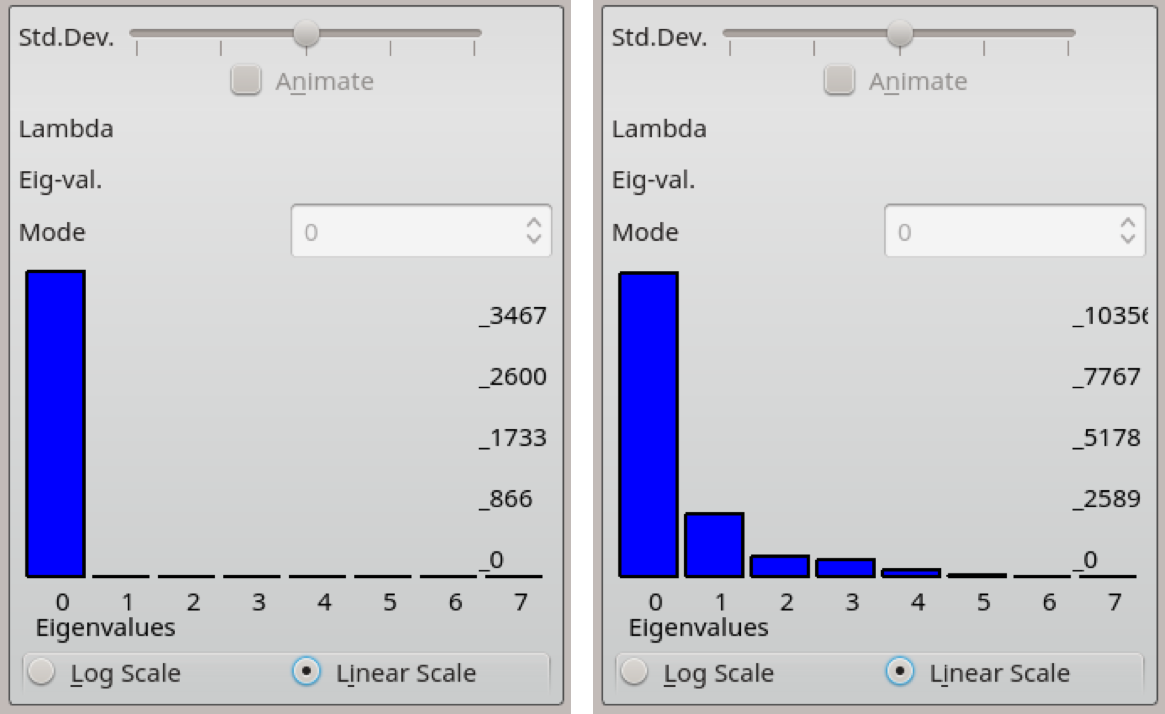
\includegraphics[width=0.6\textwidth]{figs_v2/spectrums.png}
	\caption{Eigenvalue spectrum for correspondence model of the ellipsoid dataset with one varying mode of variation using relative weighting $= 1$ (left) and $ = 0.01$ (right). Notice a more compact statistical model (left) is achieved when balancing the trade-off between surface sampling and particle correspondence, reflecting the fact that particles are in better correspondence compared to using low relative weighting for shape correspondence }
	\label{fig:specturms}
\end{figure}

\begin{itemize}
	\item[-] \textbf{PCA:} Display the computed shape from an eigen value and a standard deviation.
	\item[-] \textbf{Std.Dev.:} Slide the slider back and forth to display the computed shape with various standard deviations.
	\item[-] \textbf{Animate:} Check this box to watch the shape morph between various standard deviations automatically. Depending on the machine running the application, the number of samples, and the size of the samples, the animation may be slow at first while building and caching the meshes. You can select the caching, memory, and threading options in the Preferences. Changing the number of neighbors, spacing, and smoothing options in preferences also affects meshing time and quality.
	
\item[-] \textbf{Mode:} This selects the ordered eigen vector and eigen values from the statistical analysis. There are number of samples - 1 modes. The higher the mode, the less variance with the standard deviations. Usually the first hand full of modes contain the most variance between shapes.

\item[-] \textbf{Log Scale vs. Linear Scale:} The bar graph, displaying the eigen values spectrum of the optimized model, can be plotted in either log or linear scaling. The graph shows the eigen values in decreasing values to depict statistical relevancy. Fig. \ref{fig:specturms} shows the spectrums of the optimized models using relative weight 0.01 and 1 respectively for the ellipsoid samples. 

\item[-] \textbf{Regression:} This option is not yet available.

\end{itemize}


\section{View options}

\begin{figure}[!htp]
\centering
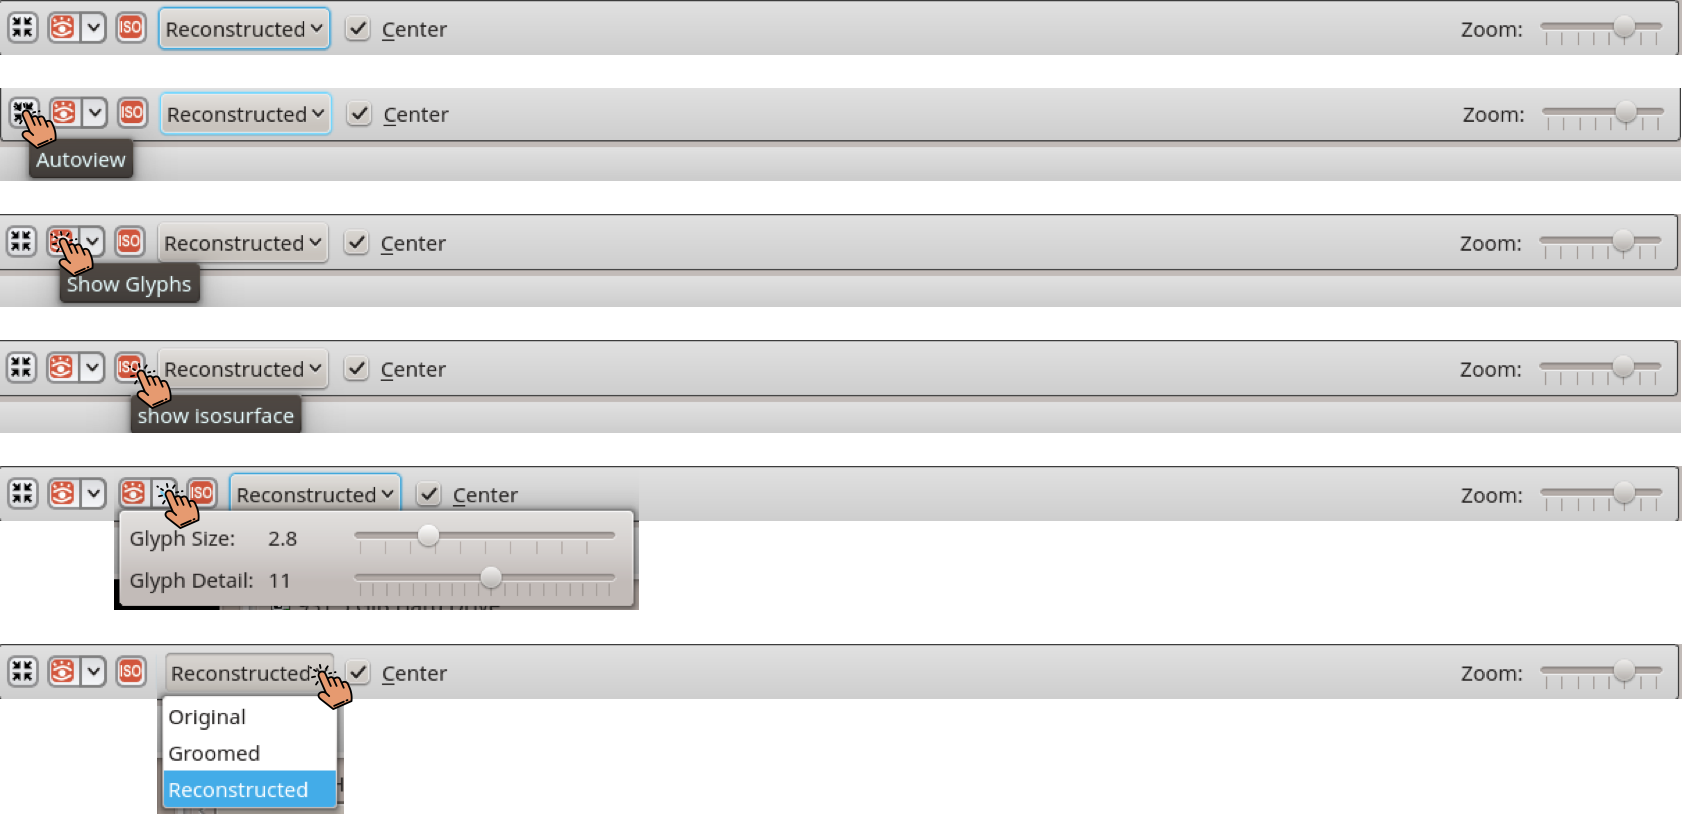
\includegraphics[width=1\textwidth]{figs_v2/render.png}
\caption{Rendering options}
\label{fig:render}
\end{figure}

The render window has a few shortcuts to viewing options (see Fig. \ref{fig:render}). From left to right, here are the rendering options:

\begin{itemize}

\item[-] \textbf{Autoview:} Reset the view to fit the samples. This only affects zoom and translation.

\item[-] \textbf{Show Glyphs:} Toggle whether to show the glyphs for the correspondence points.

\item[-] \textbf{Glyph Quality:} This slider changes the quality of the correspondence points glyphs. This is sync'd with the render window shortcut option.

\item[-] \textbf{Glyph Size:} This slider changes the size of the correspondence points glyphs. This is sync'd with the render window shortcut option.

\item[-] \textbf{Glyph options:} Click the down arrow to resize the glyphs or select the quality of the glyphs.

\item[-] \textbf{Show isosurface:} Toggle whether to view the surface representing the shape. Click the down arrow for more options. You can alter the number of neighbors, point spacing, and mesh smoothing for isosurface reconstruction.

\item[-] \textbf{View mode drop-down:} This drop-down gives 3 options for view mode. Original is the binary segmentation. You must have loaded images for this option to be available. Groomed is for the distance transform view. You must
run the groom step for this to be available. Reconstructed is for the calculated shape based on the set of correspondence points. You must run the optimize step for this to be available.

\item[-] \textbf{Center:} Center the samples automatically to align. This is useful if original samples aren't the same size.

\item[-] \textbf{Zoom:} This slider allows the user to zoom in or out to view more/less samples. This is mainly useful in the "All Samples" mode of the analysis tool. Zoom is automatically selected as a user switches between analysis modes.

\end{itemize}

\begin{figure}[!htp]
\centering
    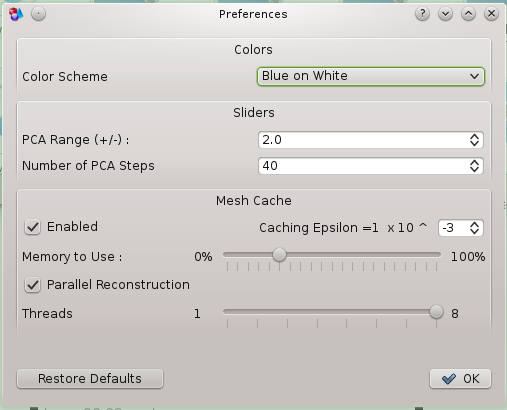
\includegraphics[width=0.5\textwidth]{figs_v2/pref.png}
\caption{Preferences}
\label{fig:pref}
\end{figure}

\section{Preferences}

\begin{itemize}
\item[-] \textbf{Color Scheme:} Select the color scheme for the rendering window.

\item[-] \textbf{PCA Range:} This is the amount of standard deviation to reach on the +/- ends of the PCA Slider.

\item[-] \textbf{Number of PCA Steps:} This determines how many steps between +/- PCA Range to take for visualization.

\item[-] \textbf{Enable Caching:} To speed up mesh animation, you can cache the meshes into system memory to load as needed.

\item[-] \textbf{Caching Epsilon:} How sensitive the caching is. The smaller the epsilon, the more meshes that will be cached, even if they are very similar. If this is too high, large mesh differences might be ignored.

\item[-] \textbf{Memory to Use:} Select the amount of system memory to use for caching. Turn this down if your machine's memory is bogged down from the program.

\item[-] \textbf{Parallel Reconstruction:} Select the amount of threads to fire (up to system hardware core max) to run while building meshes. This speeds reconstruction, theoretically.

\item[-] \textbf{Restore Defaults:} Click this to restore all options to the program's default values. Options are saved and reloaded between application runs for convenience.

\item[-] \textbf{OK:} Click this when you are done changing options.

\end{itemize}


\section{File menu}

Here you can open and save projects, load new images, open recent projects, export different studio outputs and quit the application, see Fig \ref{fig:filemenu}.

\begin{itemize}
 	\item[-] \textbf{New Project:} Start a new Studio project
 	\item[-] \textbf{Open Project:} Open a previously saved project (using its xml file). Note, in case you changed the path for a previously saved project, you will need change the corresponding paths in the xml file.
	\item[-] \textbf{Save Project:} Save the current project
	\item[-] \textbf{Save Project As:} Save the current project as a new project. This is helpful in case you wanted to save Studio output for different combination of parameter settings. You could also change the location of a previously saved project by opening it in Studio and saving it in the new desired location without having to manually change the paths in the xml file.
	
	\item[-] \textbf{Set Data Directory:} Set the data directory for where generated images will be written when a project is saved. Note that in case you want to change the path of the current project or saving it as a new project (using Save Project As), you need to set the data directory to the new path such that all Studio output will be saved in this path.
	
	\item[-] \textbf{Import Images:} Load new images
	\item[-] \textbf{Export PCA Mesh:} Export a mesh reconstructed for samples, the mean, or a variance from the mean.
	\item[-] \textbf{Export Eigenvalues:} Export the Eigen values from the sample statistics.
	\item[-] \textbf{Export Eigenvectors:} Export the Eigen vectors from the sample statistics.
	\item[-] \textbf{Export PCA Mode Points:} Export the particles per PCA model to text files.
	\item[-] \textbf{Export Parameter XML:} Export an XML parameter file to run a command line too on more images
	\item[-] Open recent projects
	\item[-] \textbf{Quit:} Quit the application. 
\end{itemize}

\begin{figure}[!htp]
	\centering
	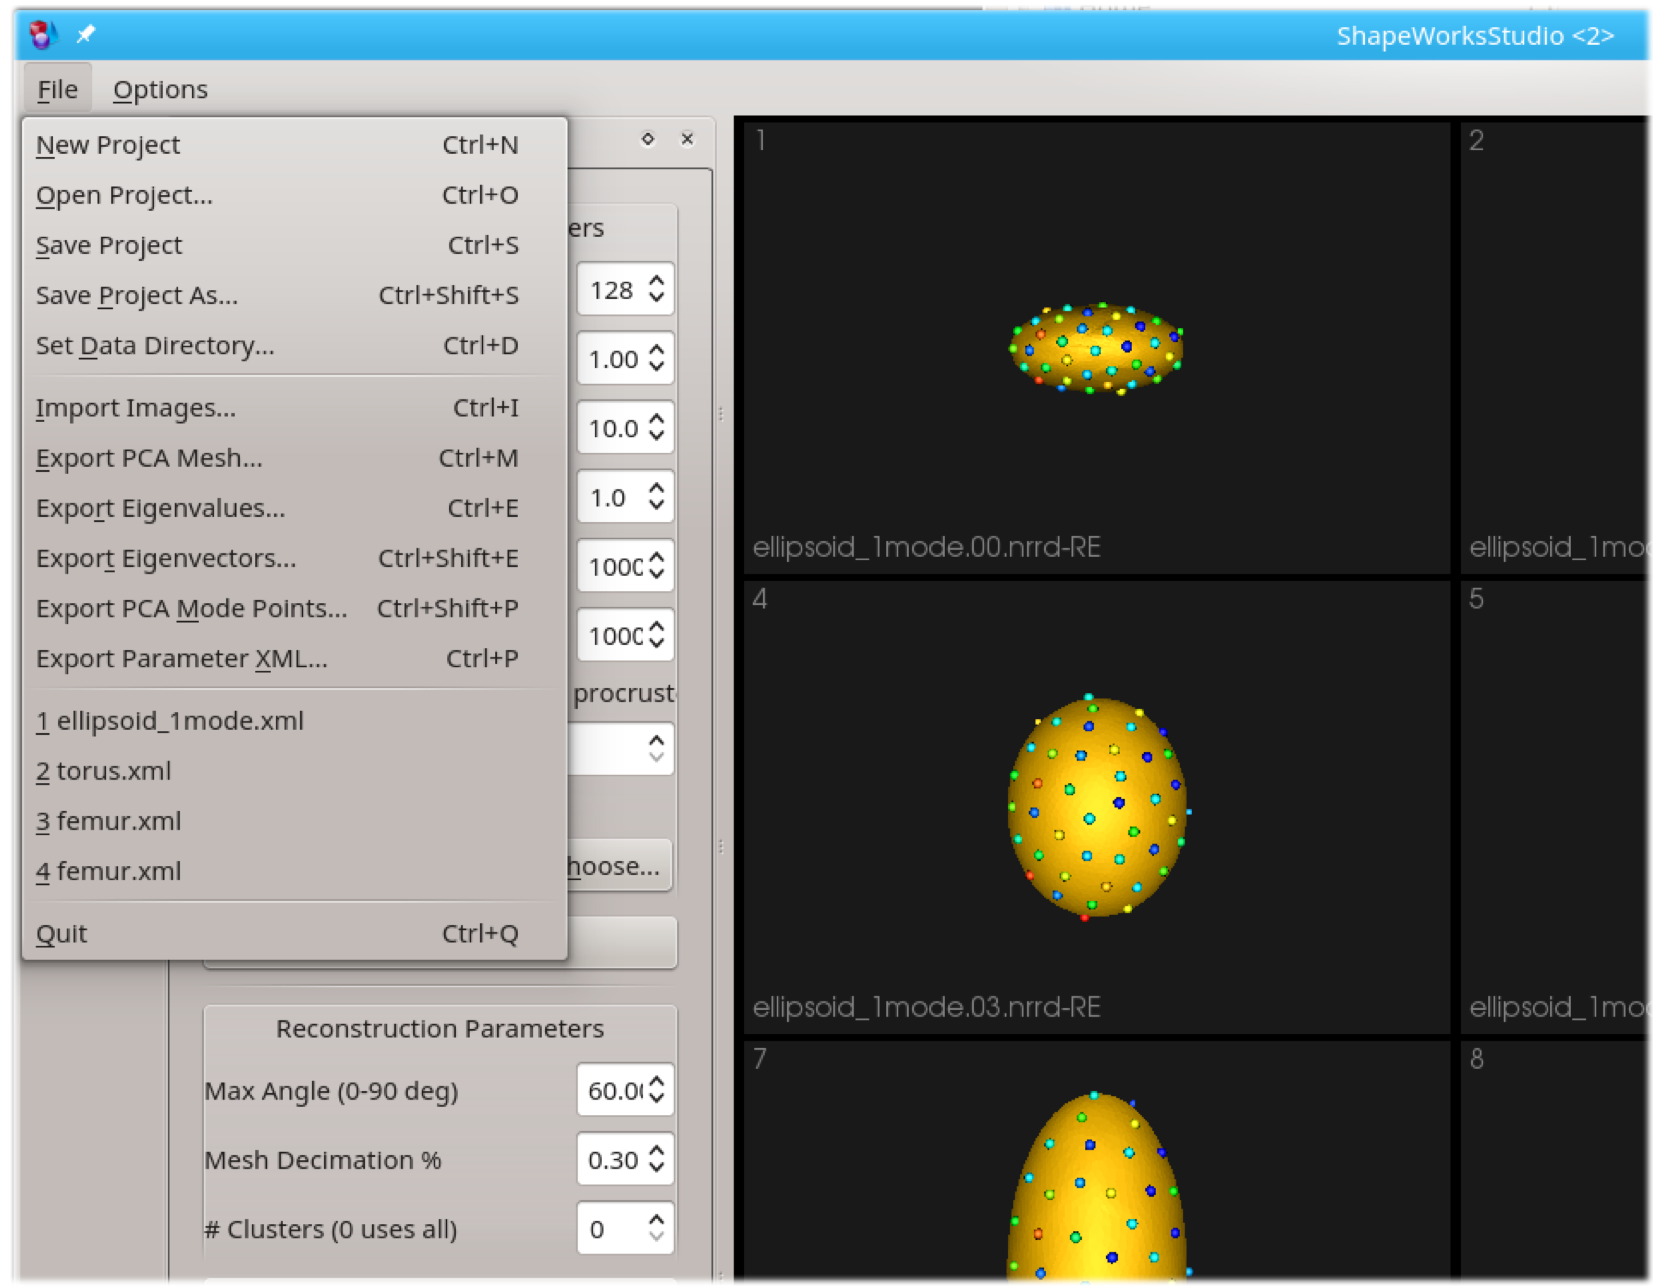
\includegraphics[width=0.7\textwidth]{figs_v2/filemenu.png}
	\caption{File menu}
	\label{fig:filemenu}
\end{figure}

\section{Tutorial 1: torus example}

This tutorial will illustrate how to use the ShapeWorksStudio software to optimize correspondences on image segmentations (i.e., binary volumes), which are a common format in many shape studies that rely on 3D imaging to extract anatomy. In this example, we will compute a statistical model of 20 synthetically generated tori. The tori are parameterized by small radii $r$ and a large radii $R$, each randomly sampled from a Gaussian distribution. The resulting shape model will therefore show two orthogonal modes, with the variance in each of these modes corresponding to that of the sampled distributions for $r$ and $R$. This tutorial proceeds step-by-step through the full analysis pipeline described in Section 3.C.  You can download this torus data (\texttt{torus\_2modes.zip}) from the Studio's release page\footnote{\texttt{https://github.com/SCIInstitute/ShapeworksStudio/releases}}. Navigate to the directory where you have downloaded this dataset and unzip it. You should now have a new directory which contains 20 synthetically generated tori, The tori are represented as binary volumes, i.e., as image segmentations. Pixels inside each torus have value 1, and pixels outside have value 0. Fig. \ref{fig:torus_data} shows the isosurfaces of the 20 tori after being loaded in Studio.

\begin{figure}[!htp]
	\centering
	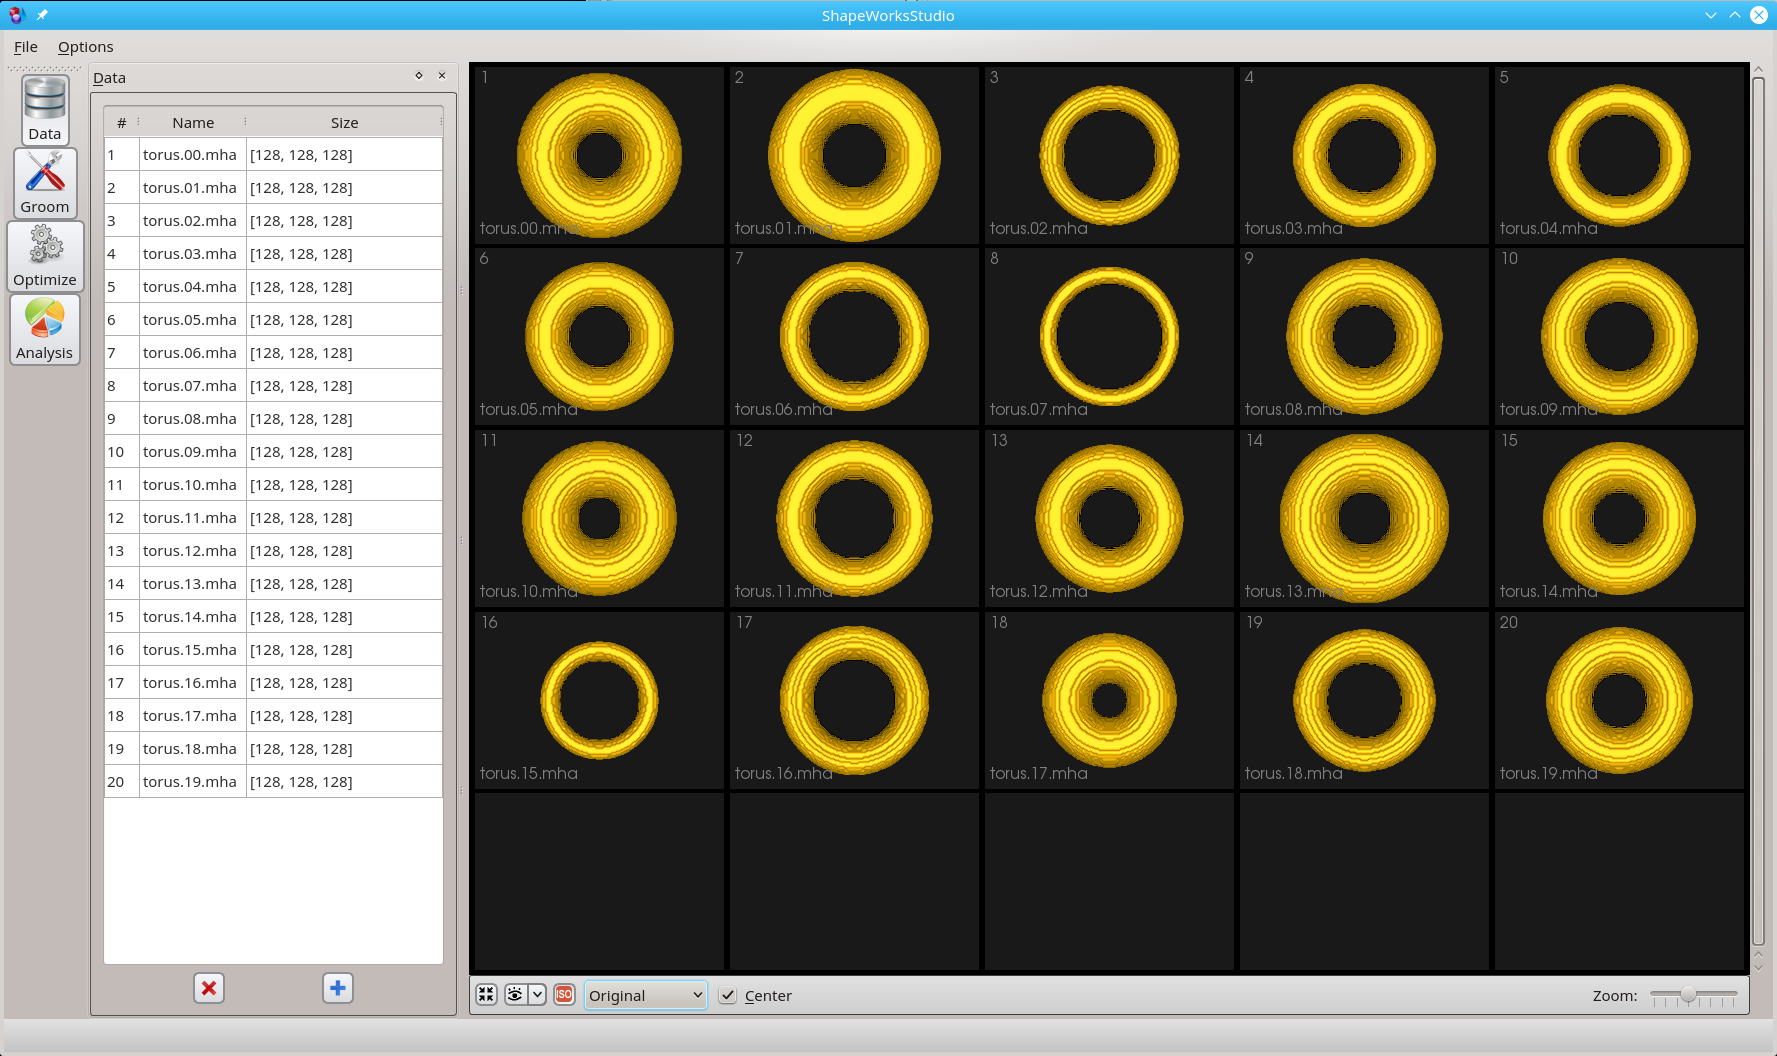
\includegraphics[width=0.9\textwidth]{figs_v2/torus_data.png}
	\caption{After loading the images: Left: the \texttt{Data} panel shows the files names and the image sizes of the 20 tori. Right: the rendering window displays the isosurface of the tori binary images that have been loaded to your project}
	\label{fig:torus_data}
\end{figure}

\subsection{Preprocessing with Groom}

As discussed in Section 10.B, the first step is to convert the binary volume into a distance transform suitable for use with correspondence optimization (i.e., \texttt{Optimize}). We will do this using the \texttt{Groom} panel to perform a set of filtering operations. The first set of preprocessing steps includes shifting the center of each volume to the center-of-mass of the segmentations. This establishes a common coordinate frame, an initial, rough translational alignment. Note that, Studio assumes that all loaded images have a common image volume size. Note that if the shapes embedded in your own image volumes are already in alignment, then this operation is not needed. In the case of the torus data, this step is also not necessary, but is illustrated here because it may be generally useful for real-world data. Next, we will perform morphological operations to isolate the foreground and fill any existing holes in the segmentations. This preprocessing step should take less than 5 minutes to run, depending on the speed of your computer. For segmentations that might be in a close proximity to volume boundaries, it is recommended to pad zero-valued voxels in each volume dimension. For the torus data, we pad 10 voxels (program default). 

The second  set of preprocessing steps starts with antialiasing the binary surface, and then computing a distance transform from that surface using the fastmarching method. Finally, we blur the distance transform slightly to get rid of high-frequency artifacts. This dataset contains a couple of thin tori (for example \texttt{torus.07.mha}) whose geometries are affected by the Gaussian blurring \texttt{Sigma} (in the Groom stage), best  \texttt{Sigma} setting would be 2. Type the following command. This step should also take less than 5 minutes to complete, depending on the speed of your computer. At this stage, you should have a set of implicit surface volumes labeled \texttt{torus.XX\_DT.nrrd} with \texttt{XX} denoting the shape sample index (see Fig. \ref{fig:torus_groom}). These new files are suitable inputs to the correspondence optimization.

\begin{figure}[!htp]
	\centering
	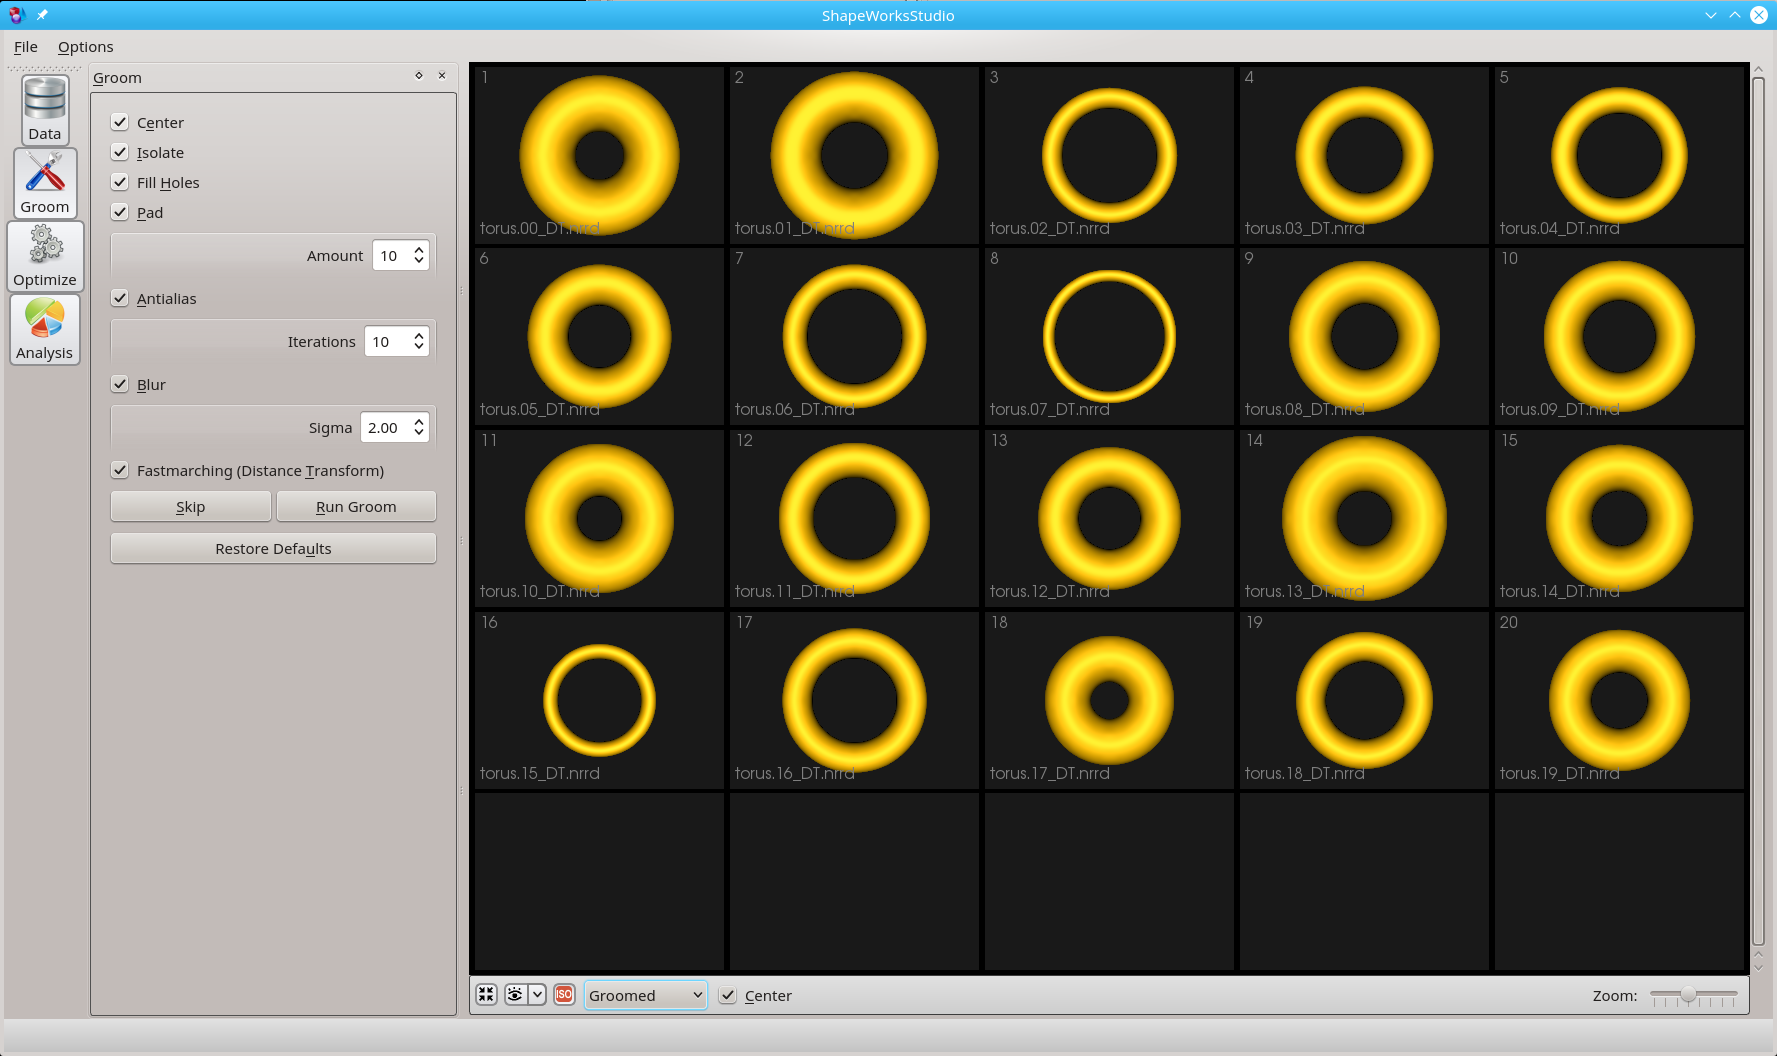
\includegraphics[width=0.9\textwidth]{figs_v2/torus_groom.png}
	\caption{Groomed tori shapes: You can switch between original and groomed shapes using the viewing options}
	\label{fig:torus_groom}
\end{figure}

\subsection{Optimizing correspondence with Optimize}

The next step is to initialize and optimize the particle system using the \texttt{Optimize} panel. In this example, we will use relatively few points, just
128 particles per torus. Correspondences are initialized on the shape surfaces using the splitting strategy described in Section 3.C, and optimized using Gauss-Seidel gradient descent on the minimum-entropy algorithm from Section 3.B. During the optimization, Studio outputs the variance associated with each of the orthogonal modes of variation in the data, obtained via principal component analysis (PCA).  As the optimization proceeds, notice how almost all of the variation in the model is shifted into the top two modes of variation. These two modes represent our two real parameters of the model, big $R$ and little $r$. The initialization and optimization process will take between 5 to 10 minutes, depending on the speed of your computer. In practice, you will need to modify the regularization parameter and the number of iterations for your data. In general, real data will require more particles per shape and more iterations for a better model fit. The relative weighting parameter, which sets $\alpha$ from
Equation 1, may also be of interest. By default, $\alpha$ is set to 1. Fig \ref{fig:torus_optimize_reconstructed} shows the optimized reconstruction model.  Figs \ref{fig:torus_optimize_reconstructed_hover1} and \ref{fig:torus_optimize_reconstructed_hover2} show visual correspondence inspection where good correspondence across different tori samples can be observed.

\begin{figure}[!htp]
	\centering
	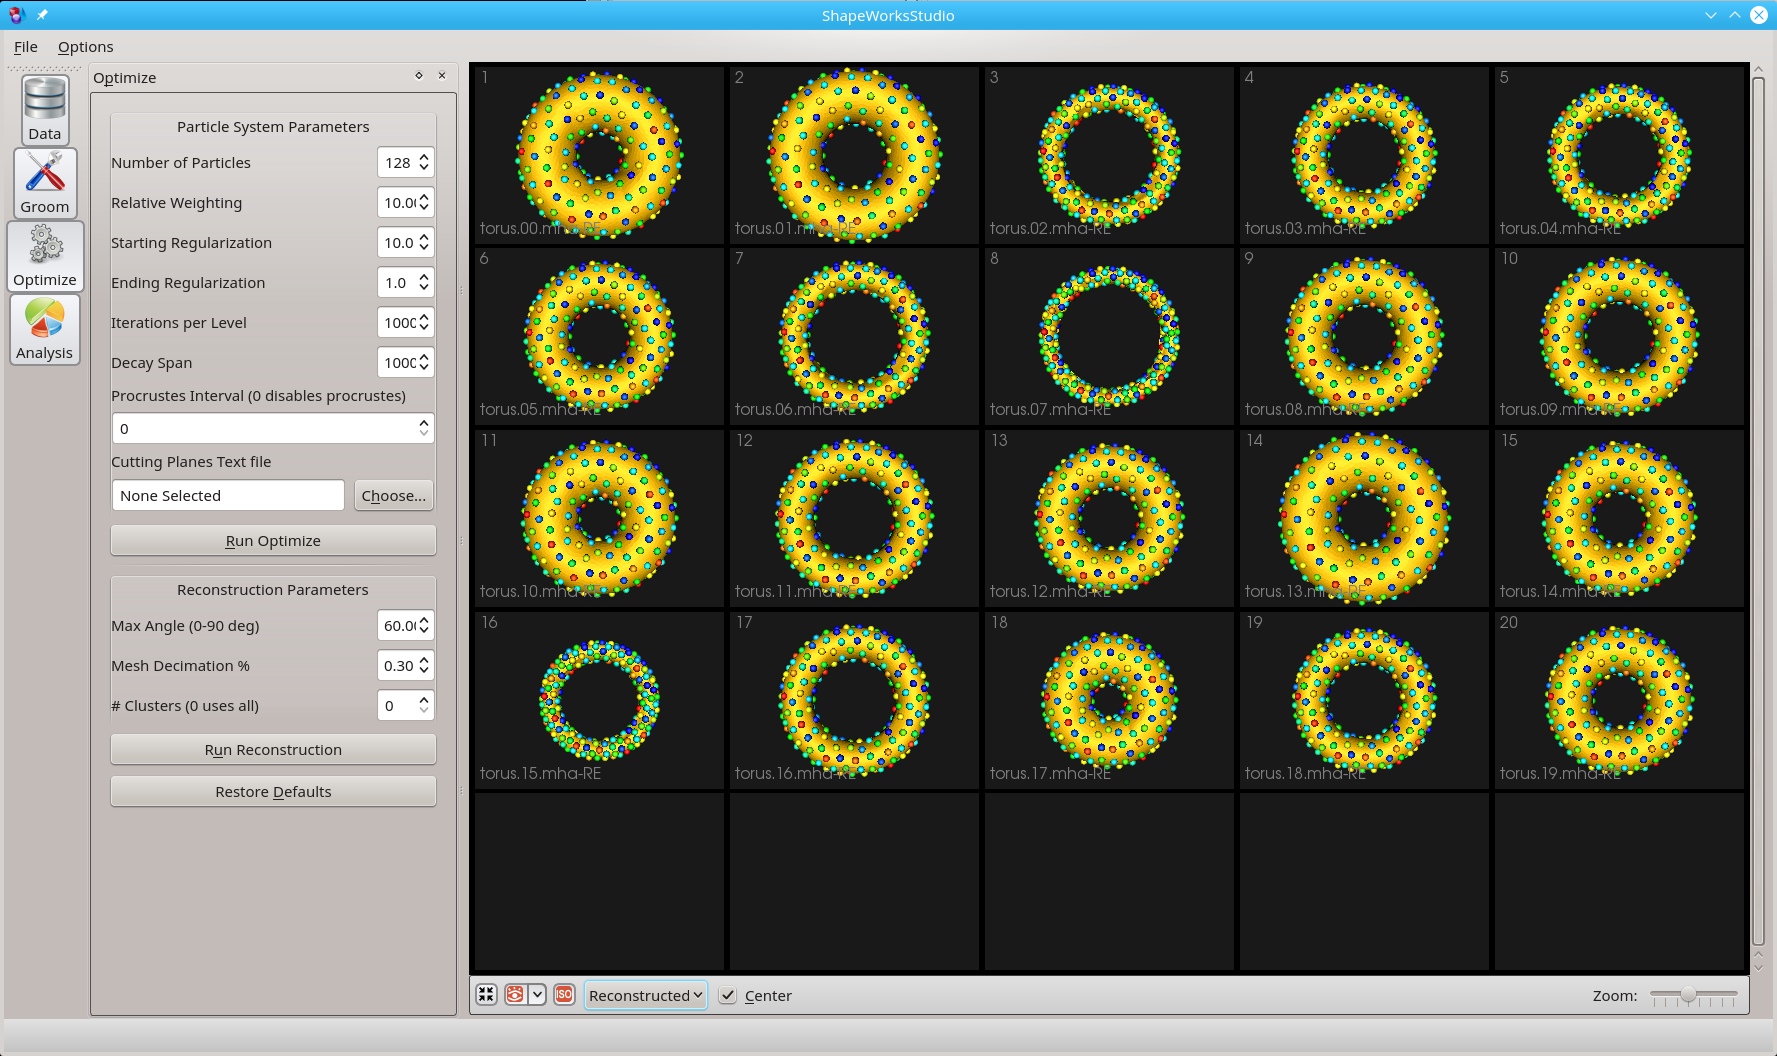
\includegraphics[width=0.9\textwidth]{figs_v2/torus_optimize_reconstructed.png}
	\caption{Optimized torus correspondence model using relative weighting $ = 1$ along with particle-based surface reconstruction.}
	\label{fig:torus_optimize_reconstructed}
\end{figure}

\begin{figure}[!htp]
	\centering
	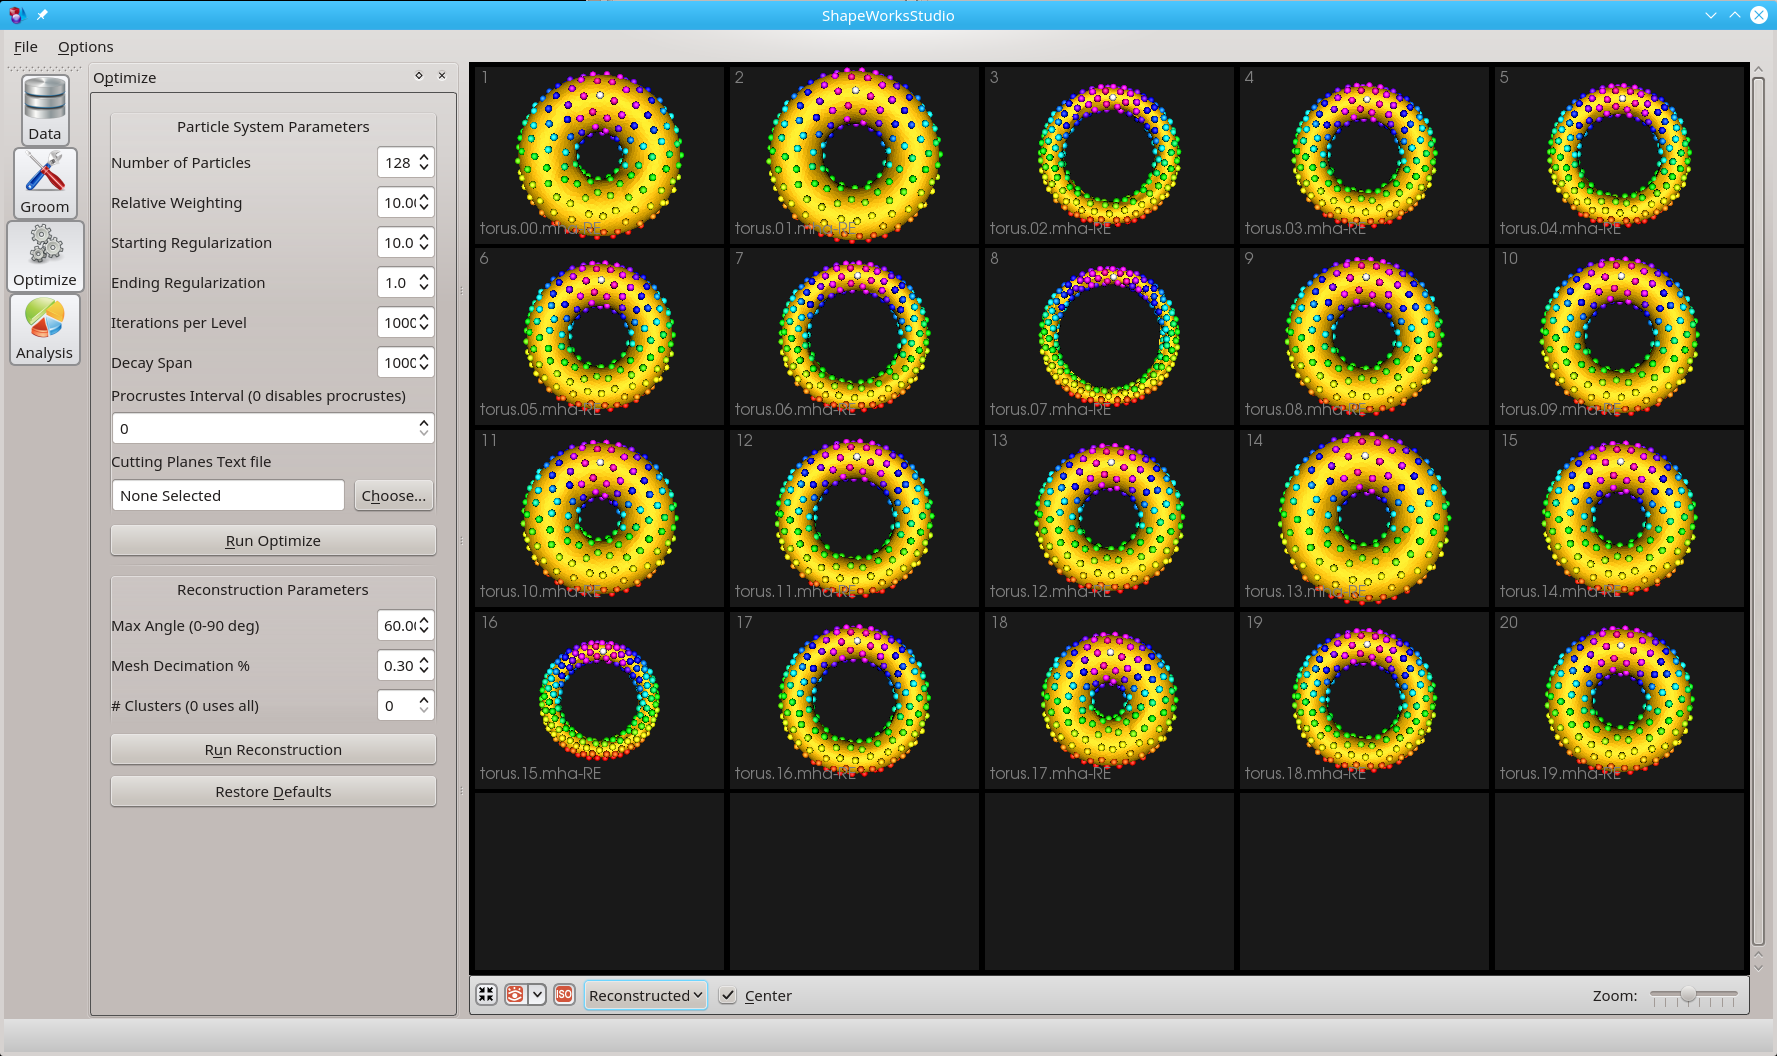
\includegraphics[width=0.9\textwidth]{figs_v2/torus_optimize_reconstructed_hover1.png}
	\caption{Optimized torus correspondence model using relative weighting $ = 1$ with one particle selected to visualize correspondence. Simply hover on the required particle and press 1, the particle will be colored in white and all other particles will be colored based on its distance to the selected particle. To recover the original display, type 1 or 2 while NOT hovering over any particles}
	\label{fig:torus_optimize_reconstructed_hover1}
\end{figure}

\begin{figure}[!htp]
	\centering
	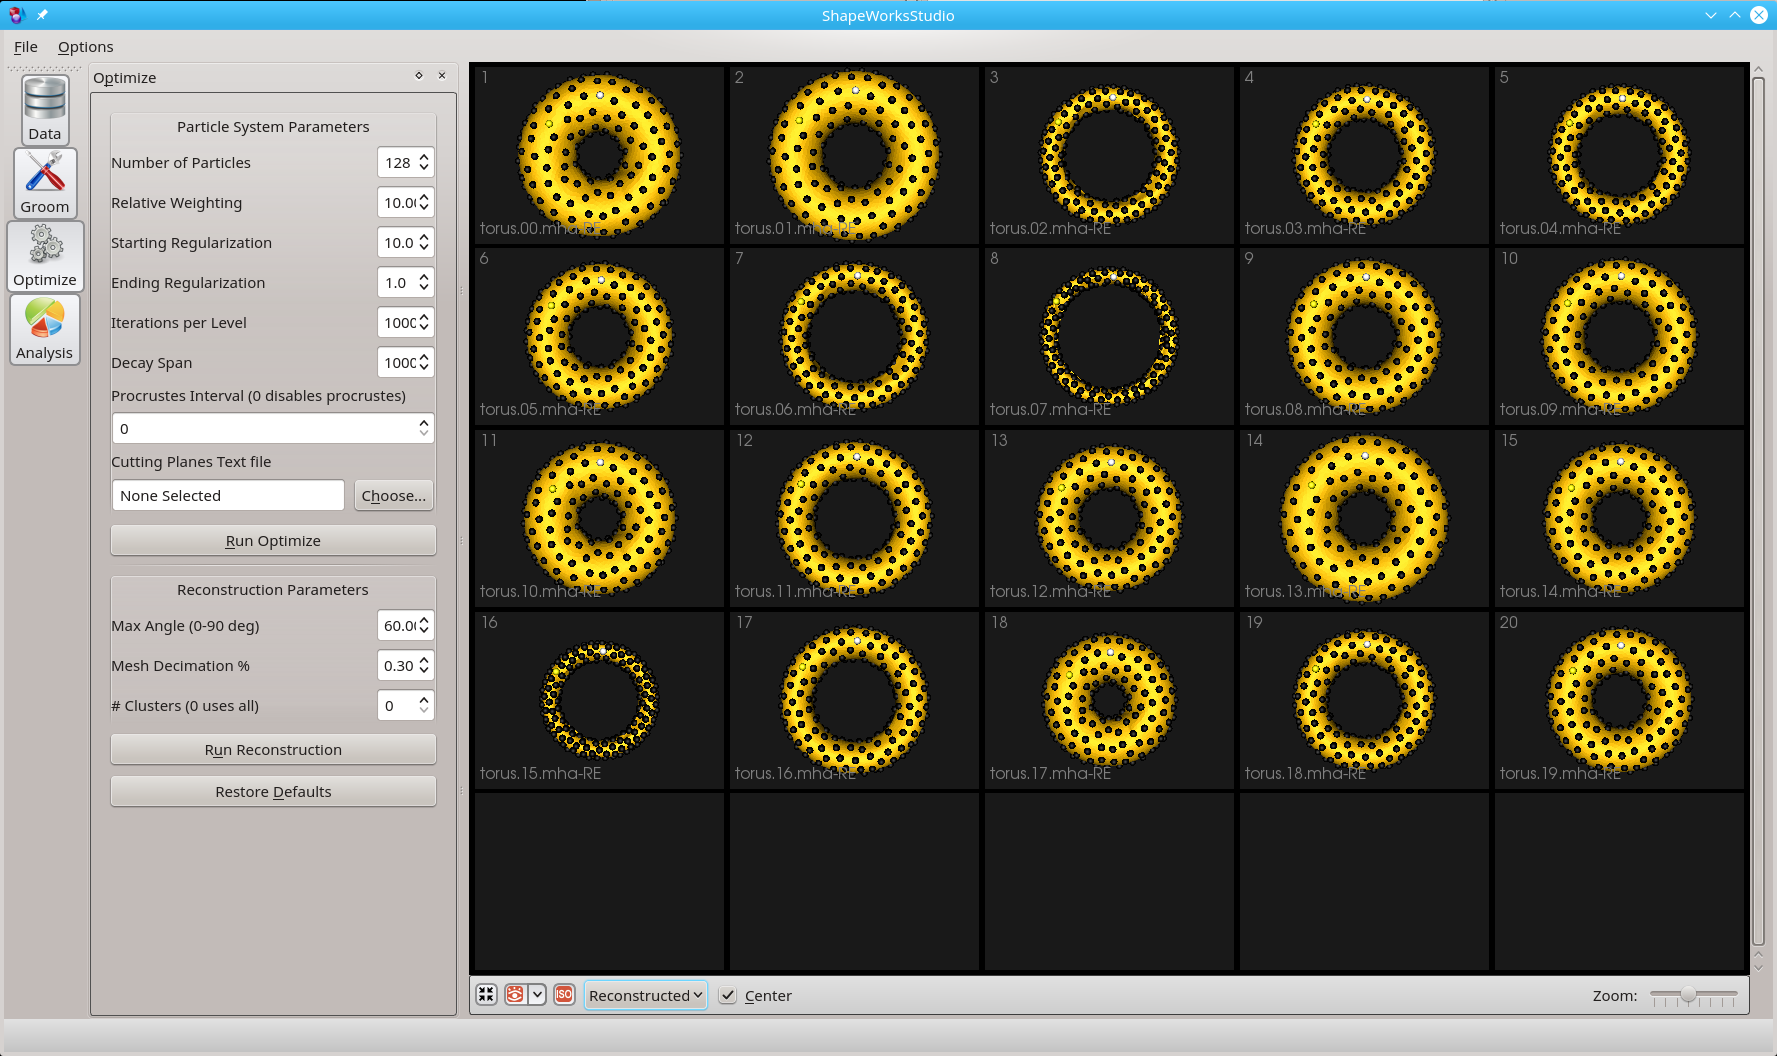
\includegraphics[width=0.9\textwidth]{figs_v2/torus_optimize_reconstructed_hover2.png}
	\caption{Optimized torus correspondence model using relative weighting $ = 1$ with two particles selected to visualize pairwise correspondence. Simply hover on the second required particle and press 2, the second particle will be colored in yellow and all other particles will be colored in black. To recover the original display, type 1 or 2 while NOT hovering over any particles}
	\label{fig:torus_optimize_reconstructed_hover2}
\end{figure}

\begin{figure}[!htp]
	\centering
	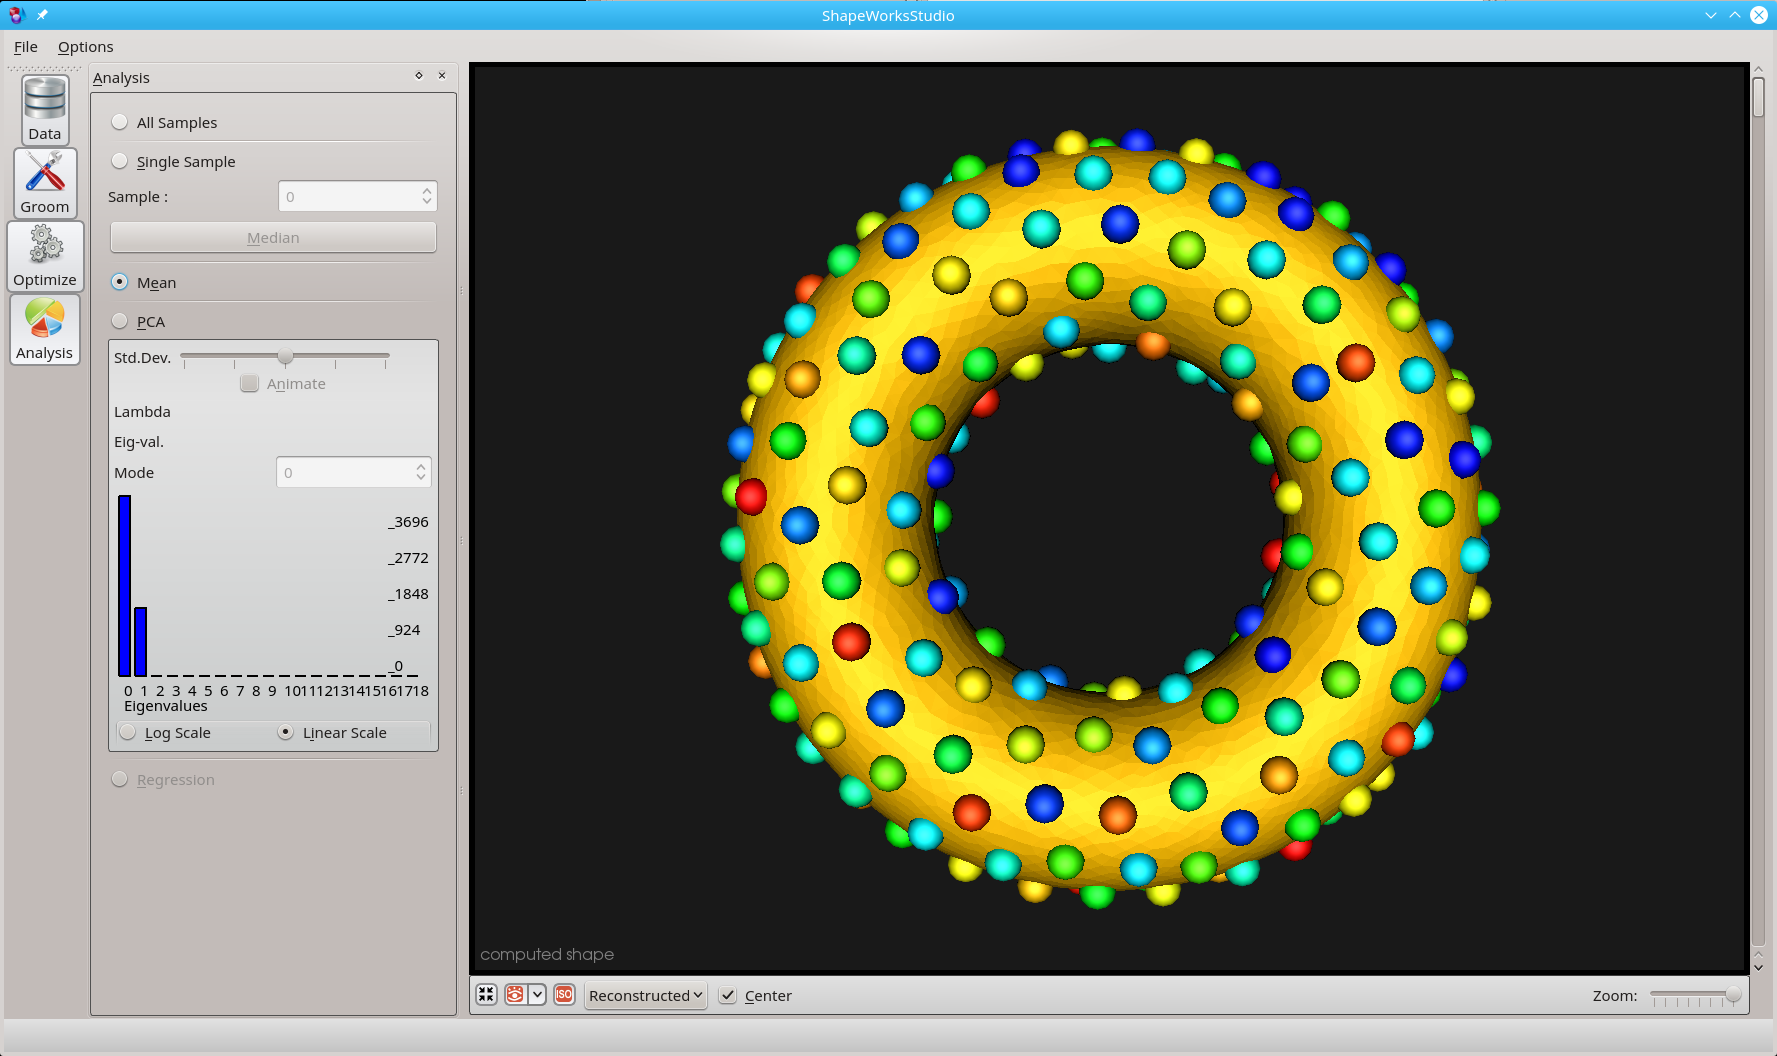
\includegraphics[width=0.9\textwidth]{figs_v2/torus_analyze_mean.png}
	\caption{ Mean correspondence positions for the ensemble of tori, and a surface reconstruction of the mean. }
	\label{fig:torus_analyze_mean}
\end{figure}


\subsection{Visualization and analysis}

We will now use the \texttt{Analysis} panel application to view the output of the correspondence optimization. By clicking the \texttt{Mean} radio button, you can see the mean correspondence positions for the ensemble of tori, and a surface reconstruction of the mean (see Fig. \ref{fig:torus_analyze_mean}). You can switch back to the correspondence points for each of the torus samples by selecting the \texttt{All Samples} radio button. Using \texttt{Single Sample}, you can scroll through each of the samples and see its correspondences and surface reconstruction. Correspondence positions are indicated by the spherical glyphs, which are colored consistently from one sample to the next to indicate correspondence. Glyph parameters can be changed using the view options (Section 11). 

Finally, we can look at the variation in the PCA modes of our model. Notice that the eigen spectrum of the torus dataset shows two dominant modes of variation. In the \texttt{Analysis} panel, choose \texttt{PCA}. Select Mode 0, the PCA mode with the largest amount of variation, and move the slider next to \texttt{Std.Dev.} box right and left. You will see that this mode corresponds to little $r$ for the torus (see Fig. \ref{fig:torus_analyze_modes}-top). The units to the left of the slider are units of standard deviation in that mode. Now select Mode 1. By moving the slider, you will see that this mode corresponds to big $R$  (see Fig. \ref{fig:torus_analyze_modes}-bottom). The remaining modes can be considered noise, and show increasingly less variation. Running
the optimization further (i.e., with more iterations per split level) for this set of data will decrease the variation in those remaining modes.

\begin{figure}[!htp]
	\centering
	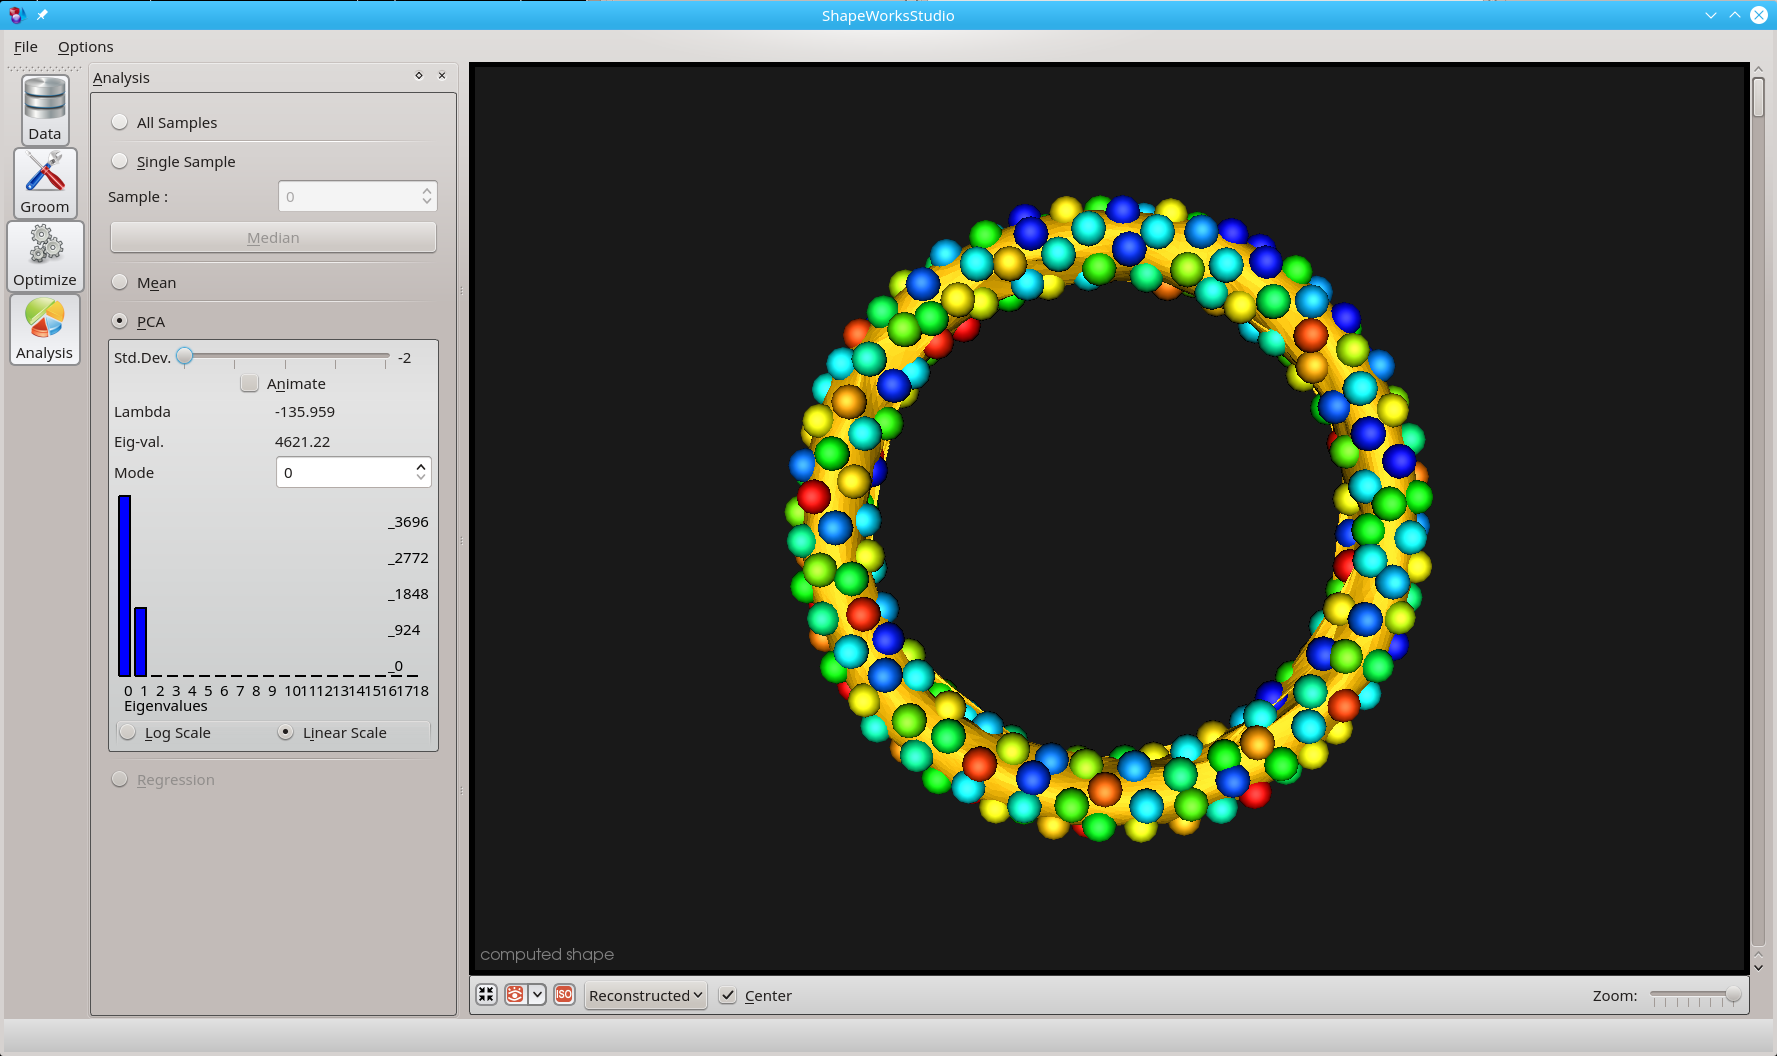
\includegraphics[width=0.32\textwidth]{figs_v2/torus_analyze_mode1_neg2std.png}
		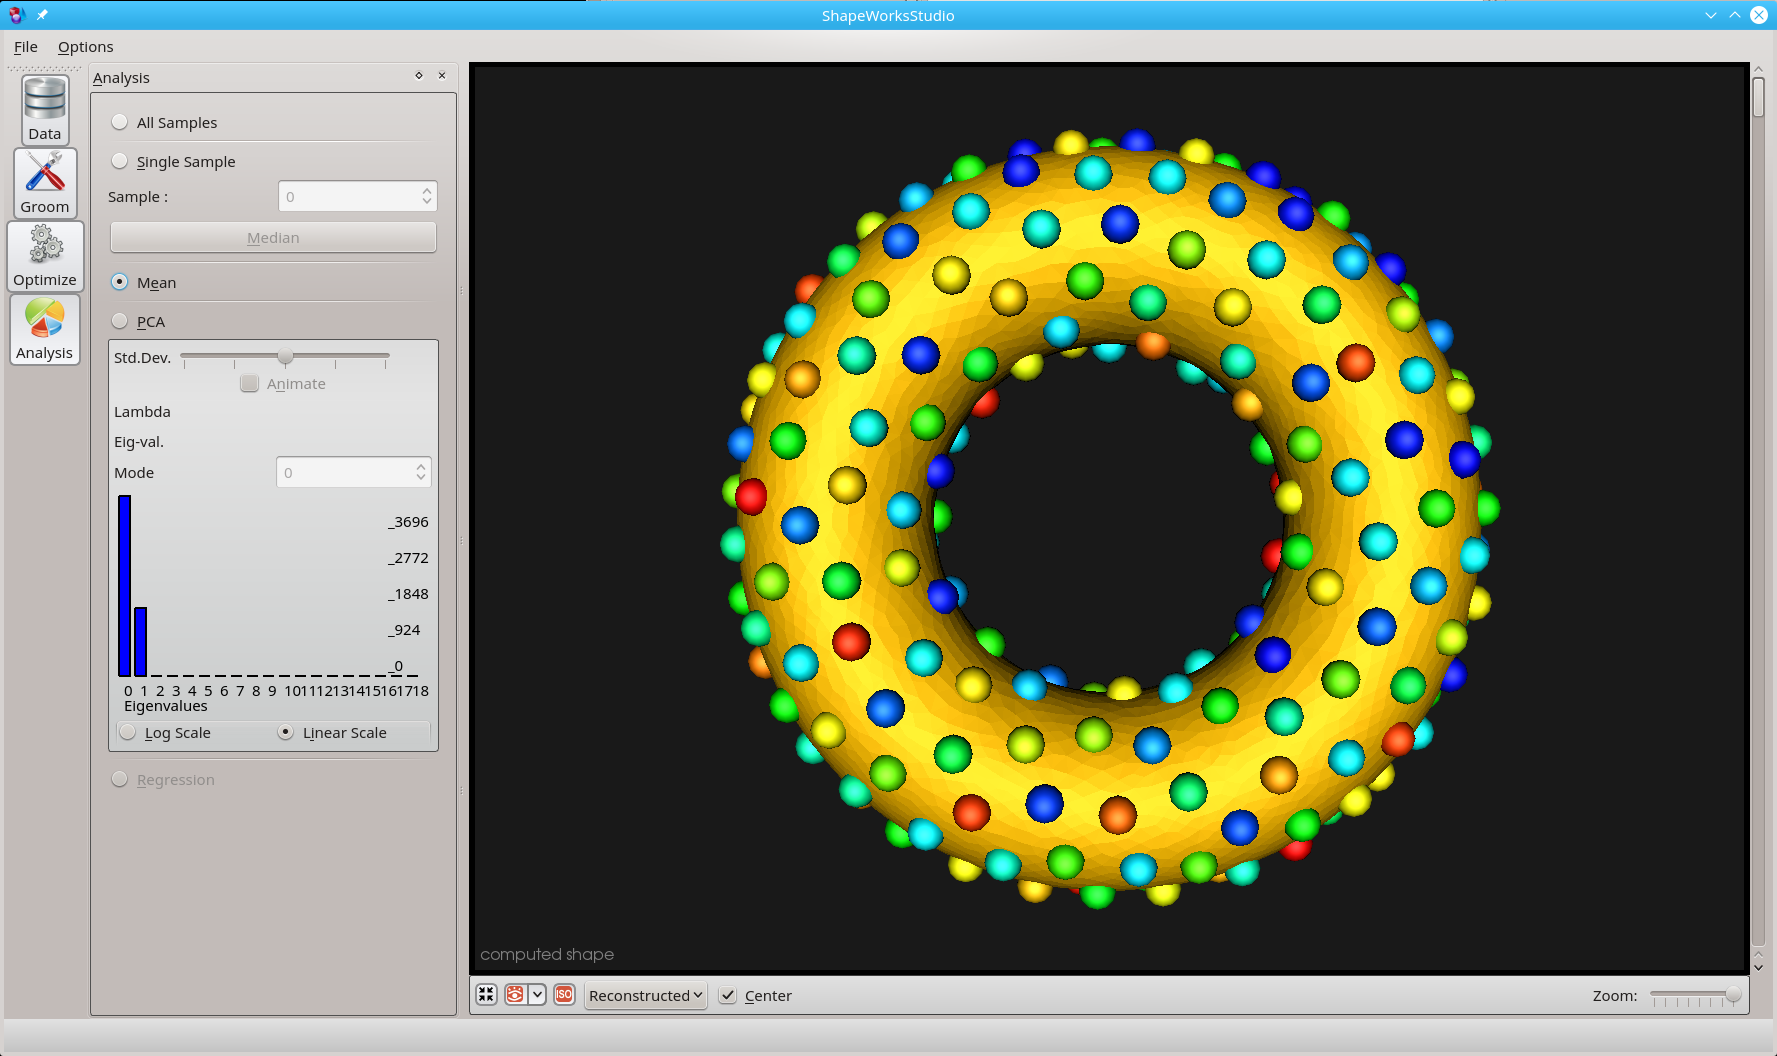
\includegraphics[width=0.32\textwidth]{figs_v2/torus_analyze_mean.png}
			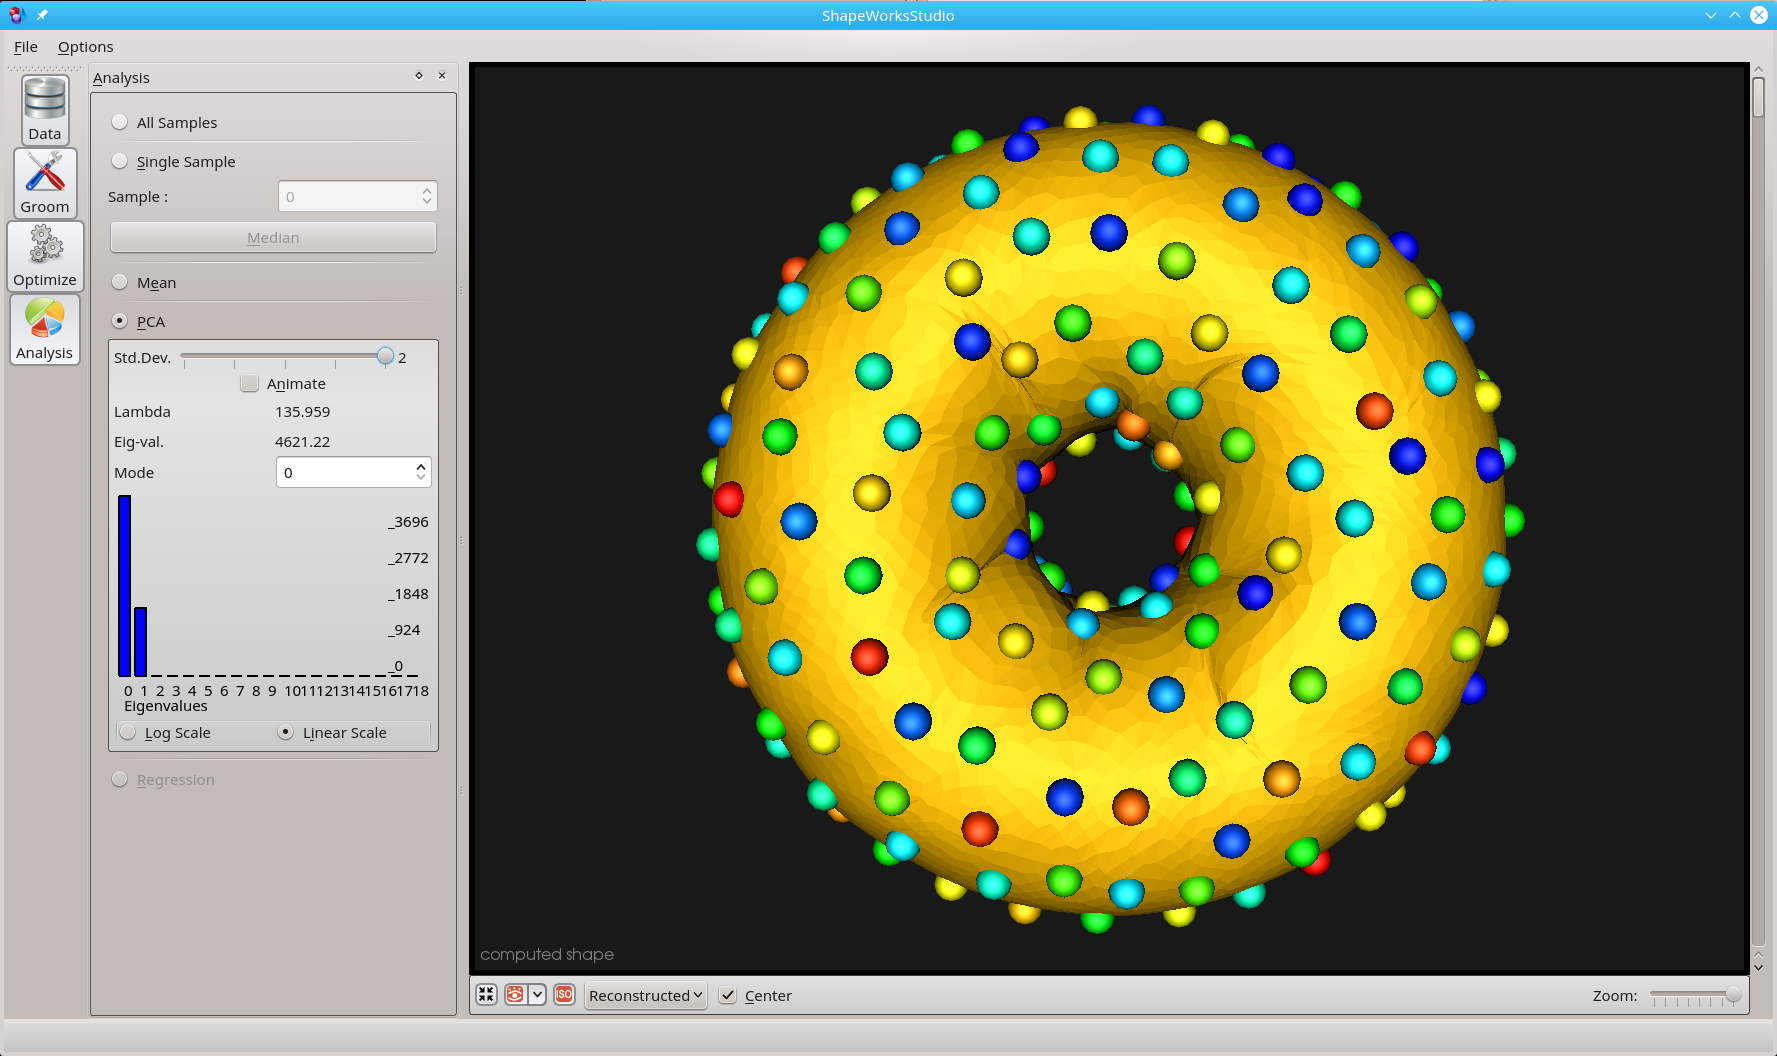
\includegraphics[width=0.32\textwidth]{figs_v2/torus_analyze_mode1_pos2std.png} \\
	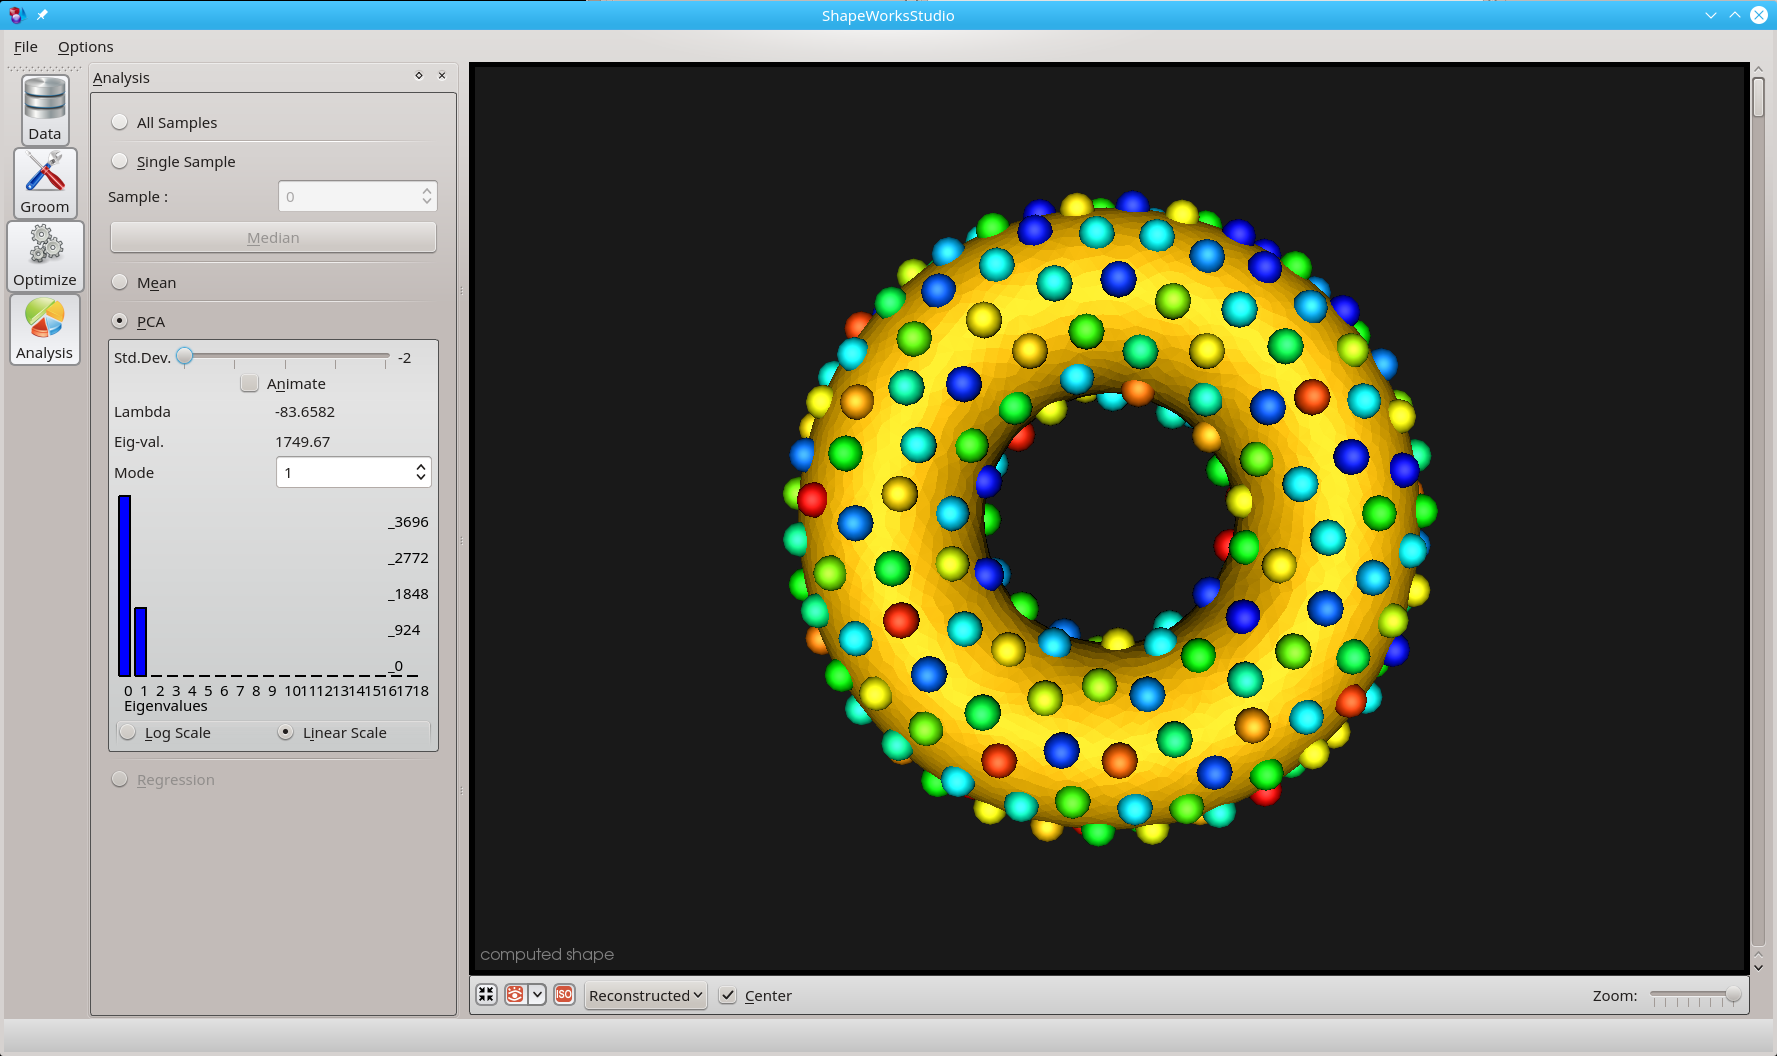
\includegraphics[width=0.32\textwidth]{figs_v2/torus_analyze_mode2_neg2std.png}
	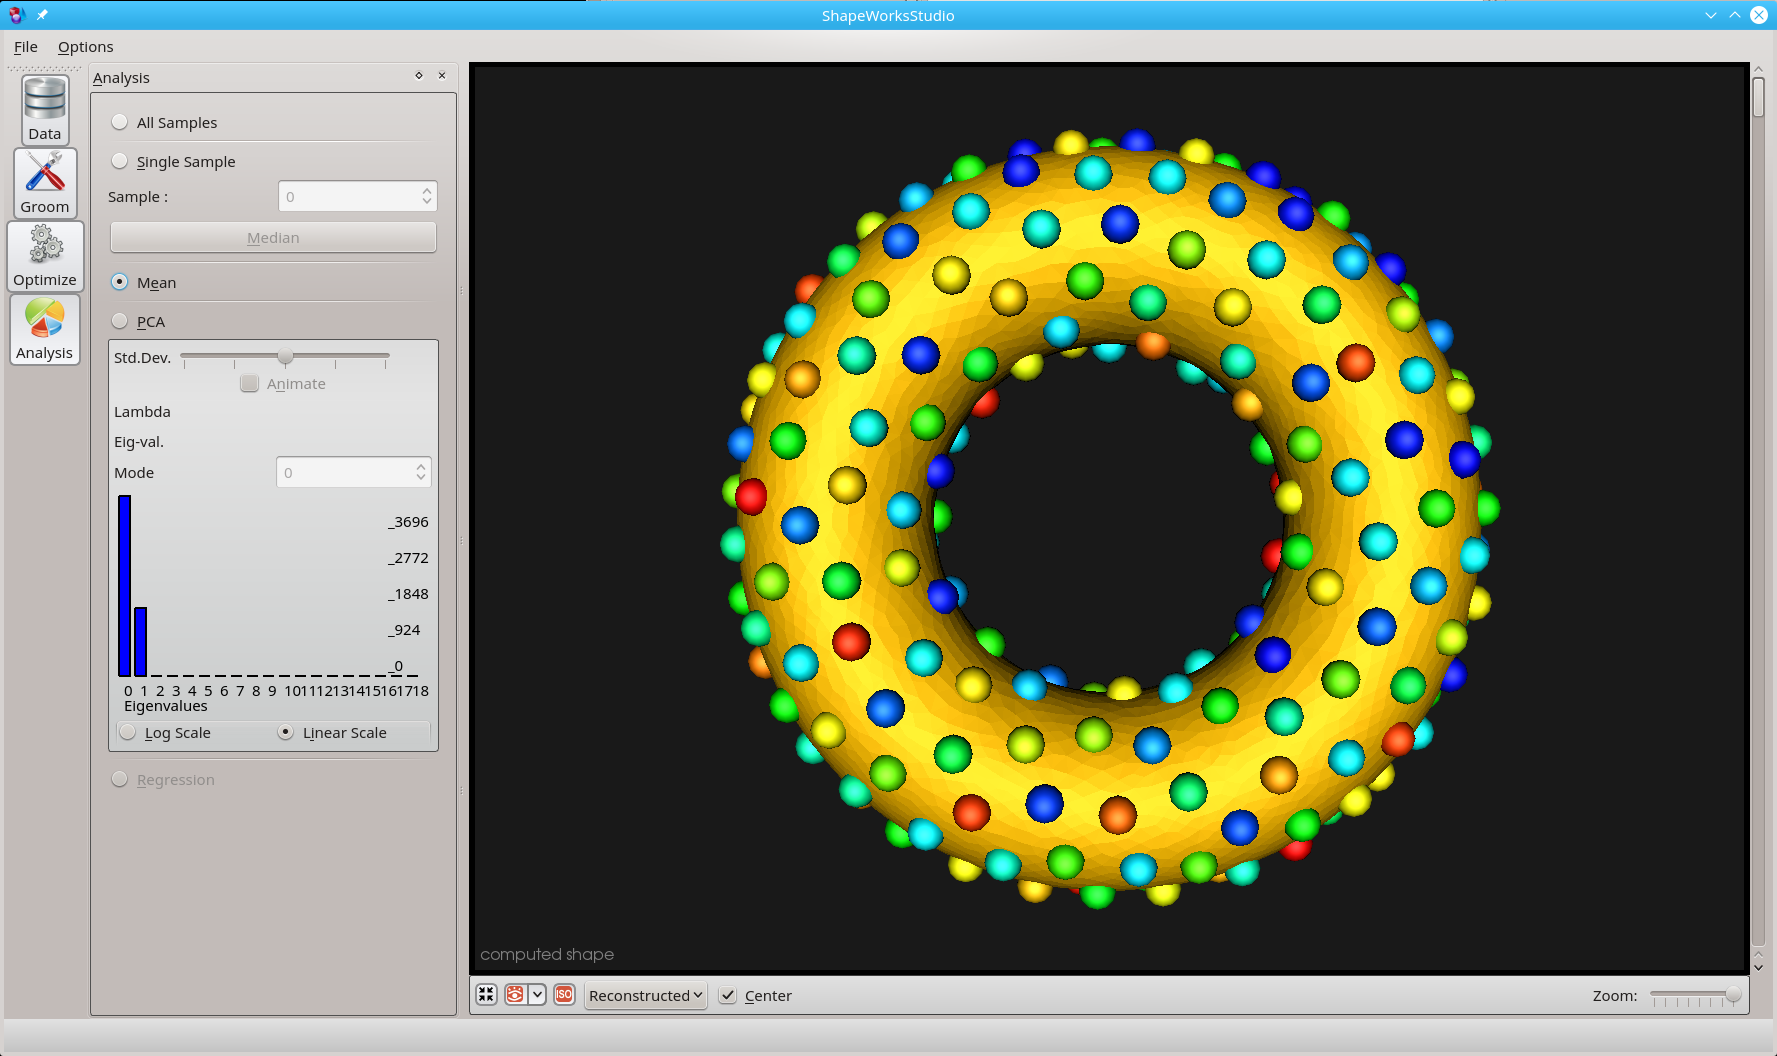
\includegraphics[width=0.32\textwidth]{figs_v2/torus_analyze_mean.png}
	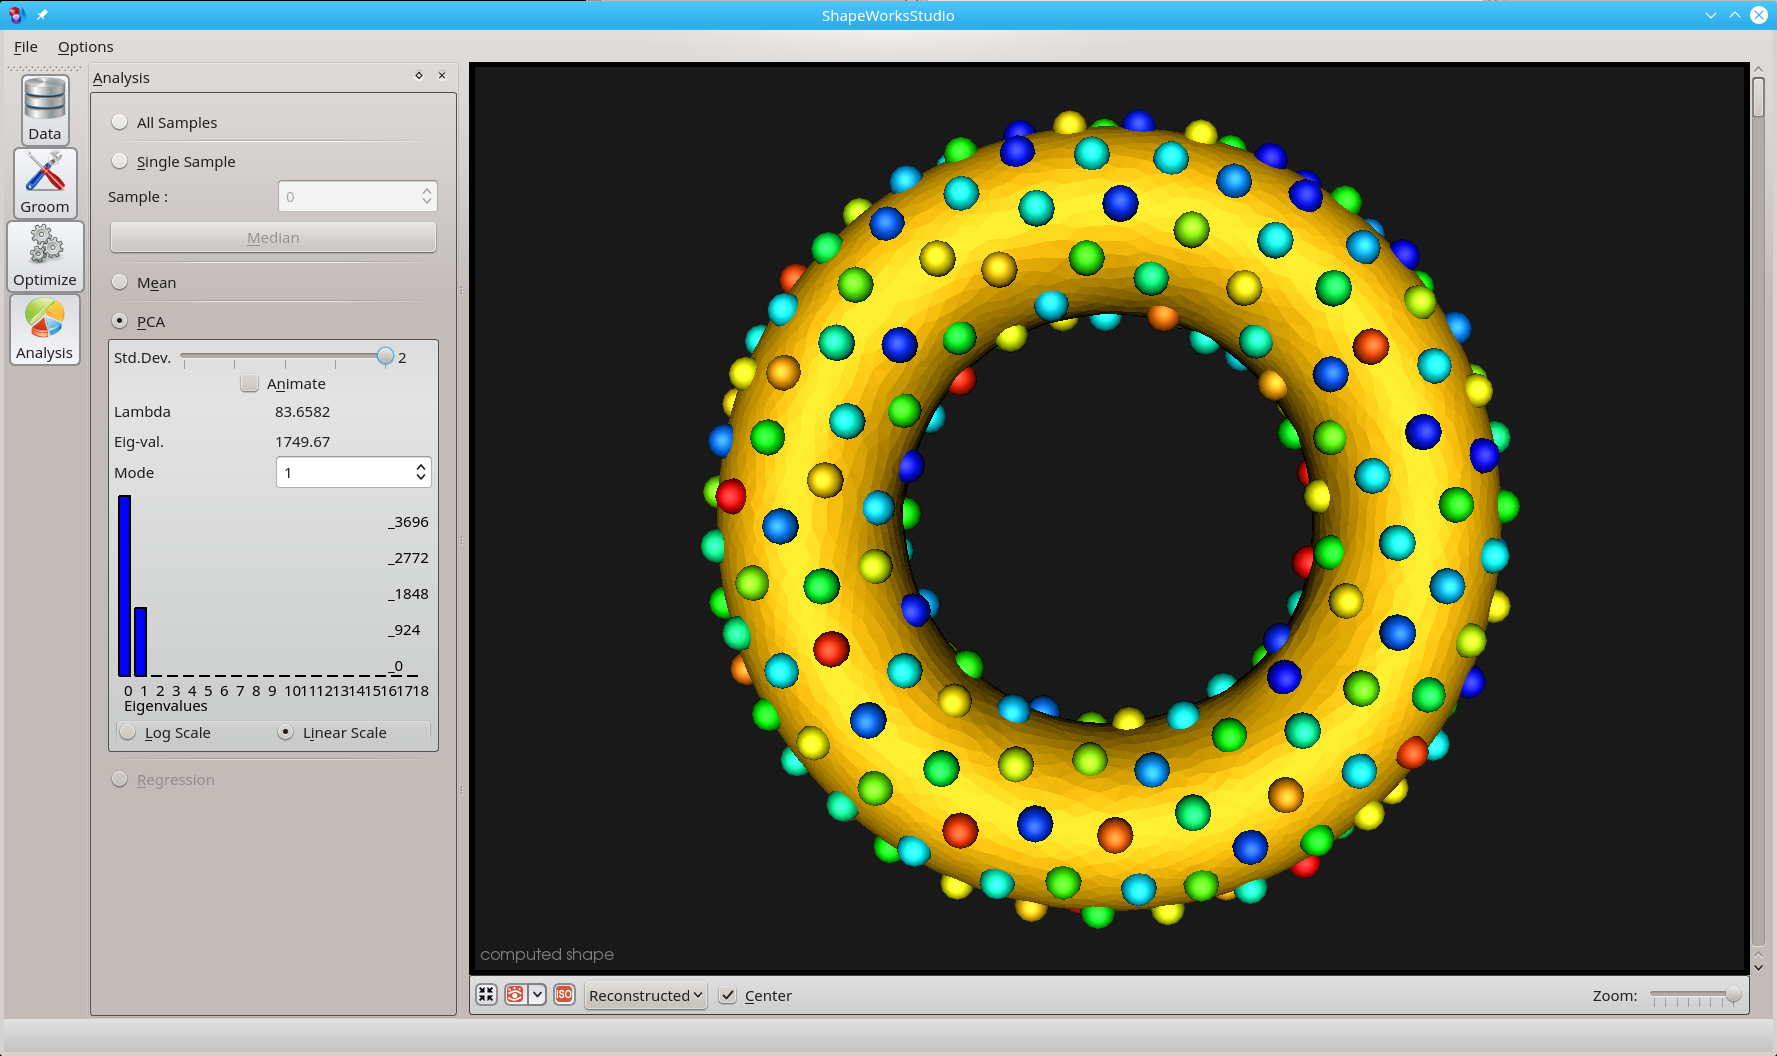
\includegraphics[width=0.32\textwidth]{figs_v2/torus_analyze_mode2_pos2std.png} 
	\caption{ Variations in PCA modes for the torus correspondence model. Top shows the first dominant mode and bottom shows the second one. Left to right shows variations in the PCA modes for -2 to 2 standard deviations. }
	\label{fig:torus_analyze_modes}
\end{figure}

\section{Tutorial 2: femur example}

In this example, we will compute a statistical model for a set of 10 healthy femurs.  You can download this torus data (\texttt{femur.zip}) from the Studio's release page\footnote{\texttt{https://github.com/SCIInstitute/ShapeworksStudio/releases}}. The main difference in the shape modeling pipeline for this particular dataset is the need for a cutting plane to limit particle distribution above the less trochanter. Figs \ref{fig:femur_data} and \ref{fig:femur_groom} show the original and preprocessed femur samples. In the \texttt{Optimize} panel, we have identified the cutting plane text file. Fig \ref{fig:femur_optimize_reconstructed} shows optimized corresponding particles whose placement is restricted to be above the provided cutting plane. Fig \ref{fig:femur_optimize_reconstructed_hover1} shows a visual correspondence inspection of a particle in the femoral fovea. Note the consistency particles coloring (which reflect distance to the fovea particle) across all samples. Fig \ref{fig:femur_optimize_reconstructed_hover2} shows a two-particles visual correspondence inspection where we have selected the second particle to be on the tip of the greater trochanter. Note that correspondence of these particles are maintained across all  the samples. Fig \ref{fig:femur_analyze_modes})shows shape variation captured in the first four modes (best seen using the animation option in studio). The first mode captures the position of the femoral fovea as well as the eccentricity of the femoral head. The second mode captures the variability in the head-neck junction. The third mode captures the curvature of the less trochanter. The fourth mode captures the shape variability of the greater tochanter.


\begin{figure}[!htp]
	\centering
	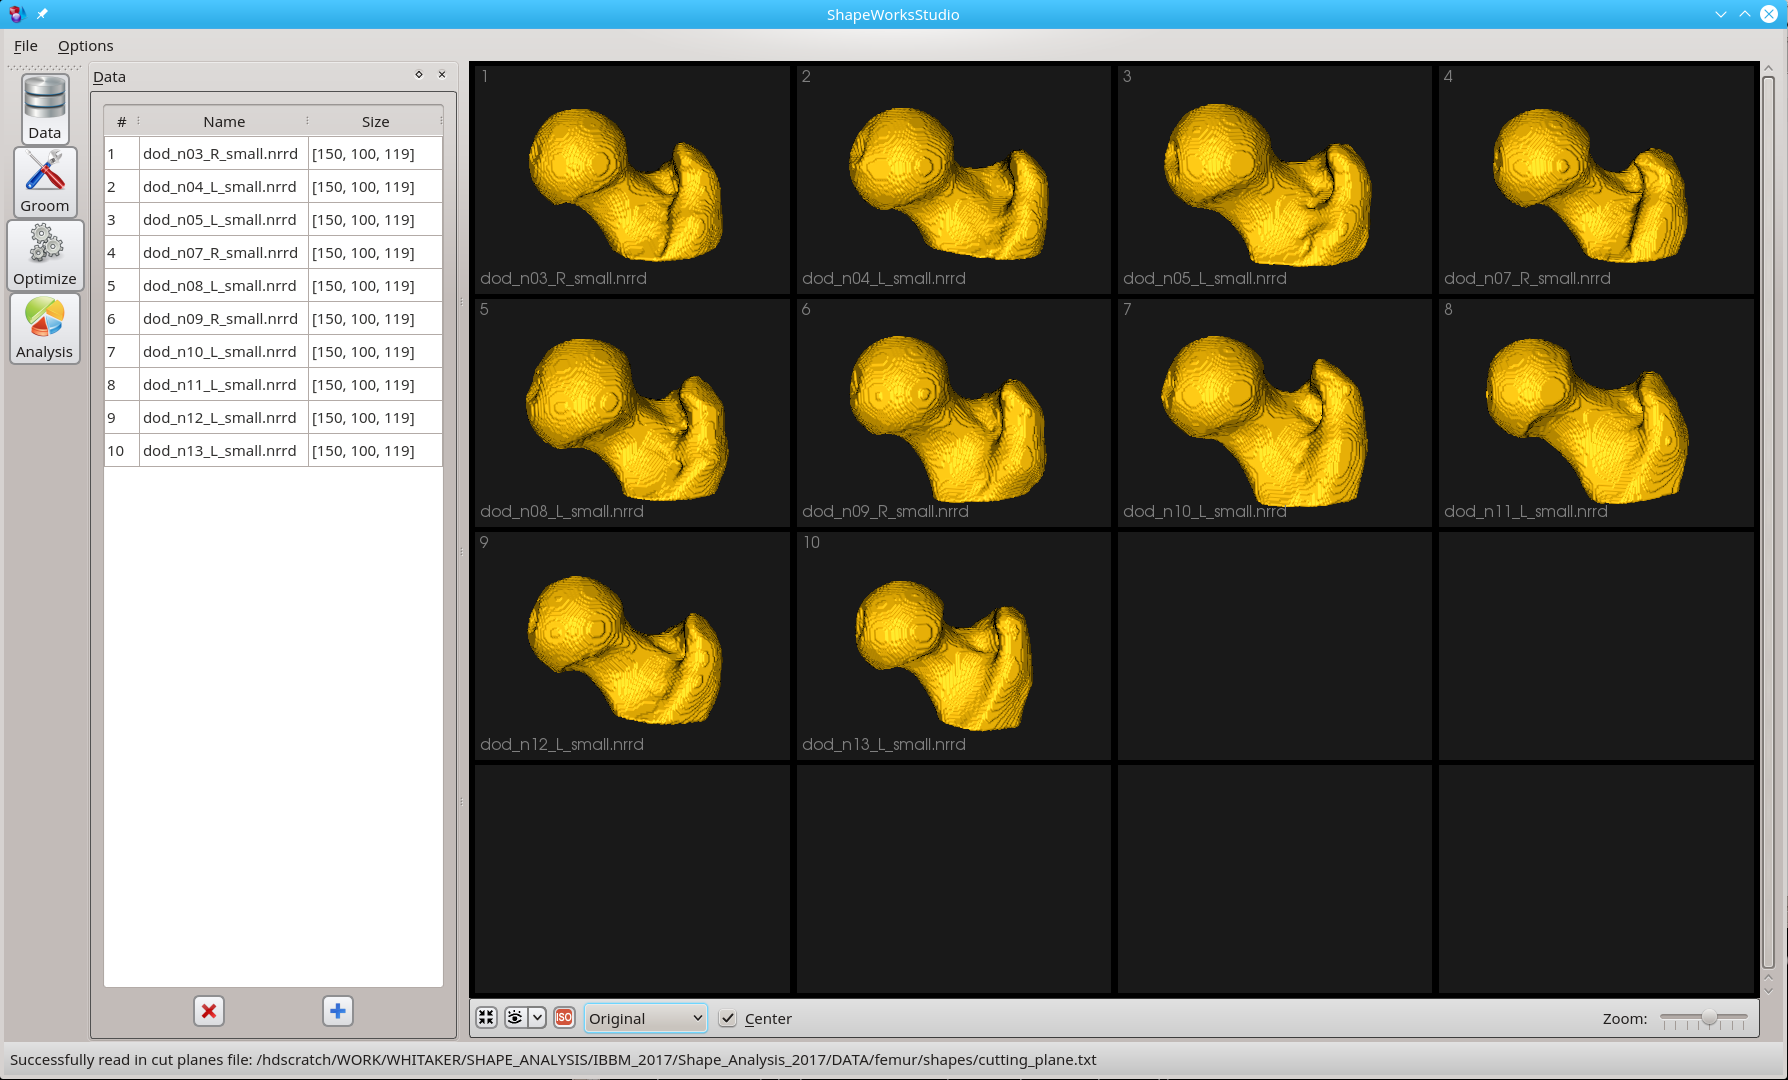
\includegraphics[width=0.9\textwidth]{figs_v2/femur_data.png}
	\caption{After loading the images: Left: the \texttt{Data} panel shows the files names and the image sizes of the 10 femurs. Right: the rendering window displays the isosurface of the tori binary images that have been loaded to your project}
	\label{fig:femur_data}
\end{figure}

\begin{figure}[!htp]
	\centering
	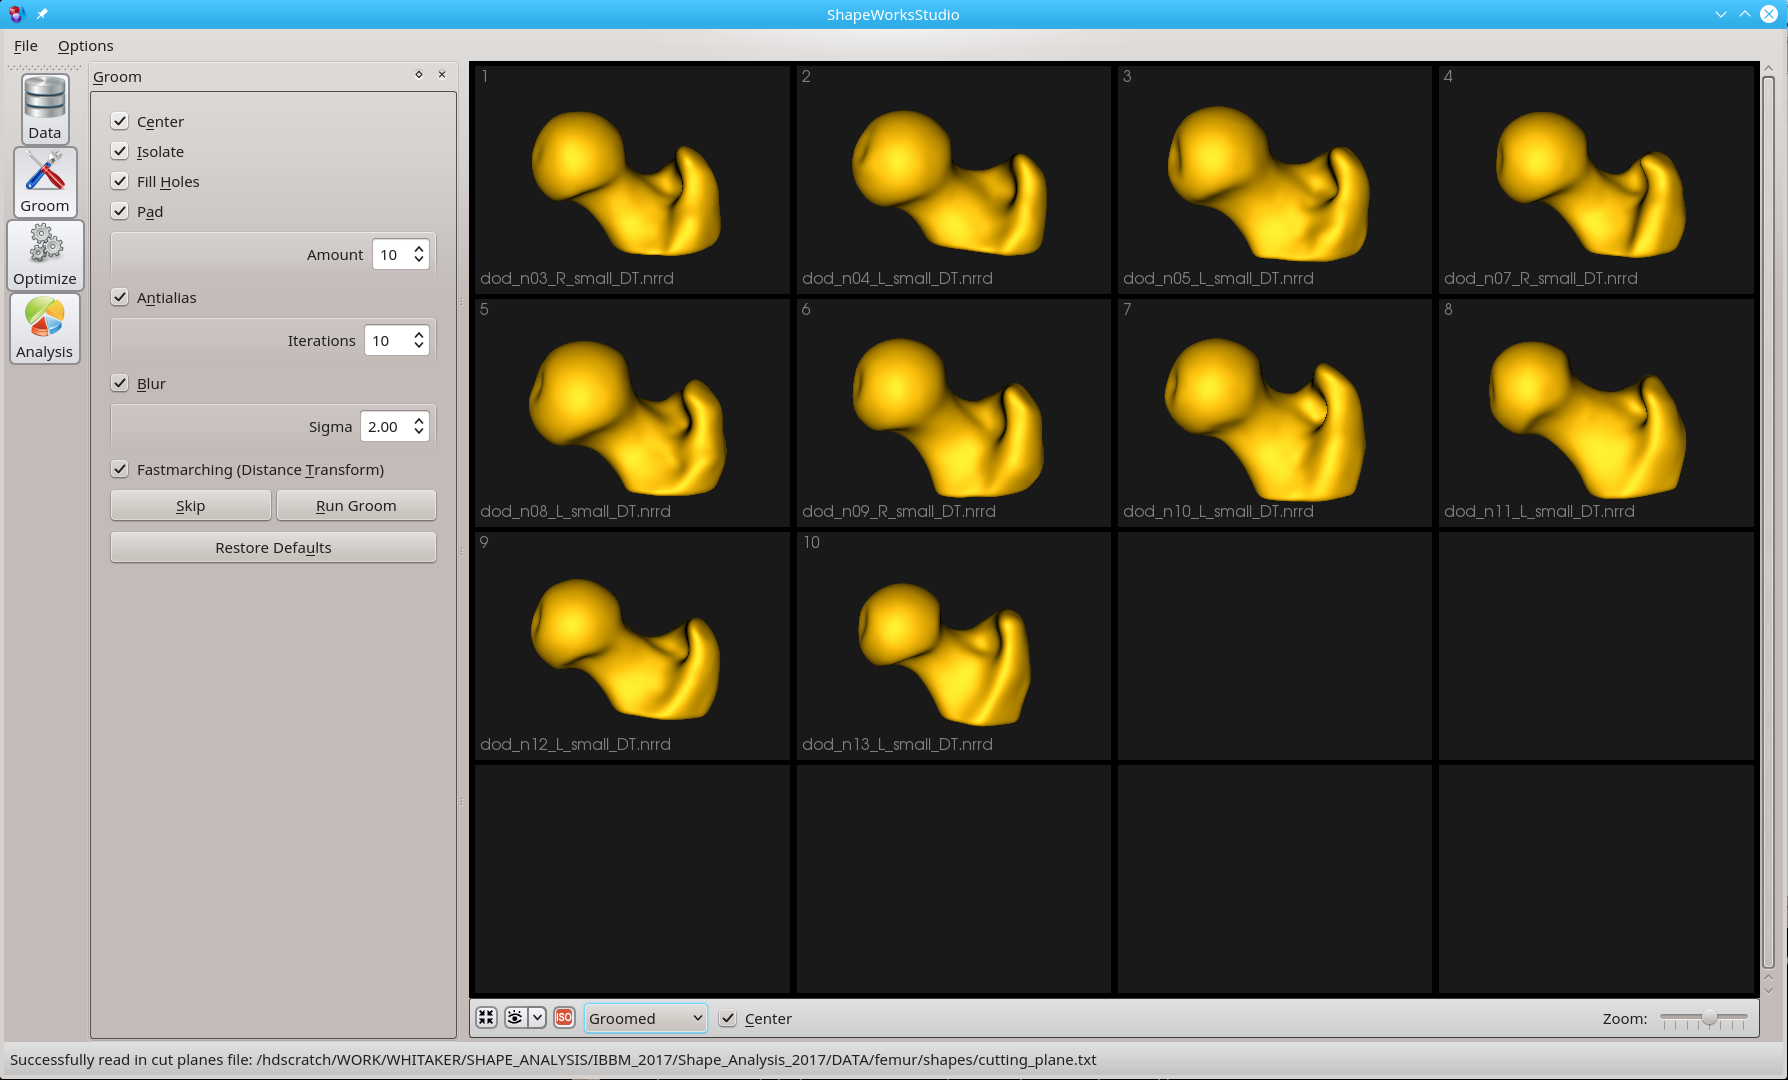
\includegraphics[width=0.9\textwidth]{figs_v2/femur_groom.png}
	\caption{Groomed femur shapes: You can switch between original and groomed shapes using the viewing options}
	\label{fig:femur_groom}
\end{figure}

\begin{figure}[!htp]
	\centering
	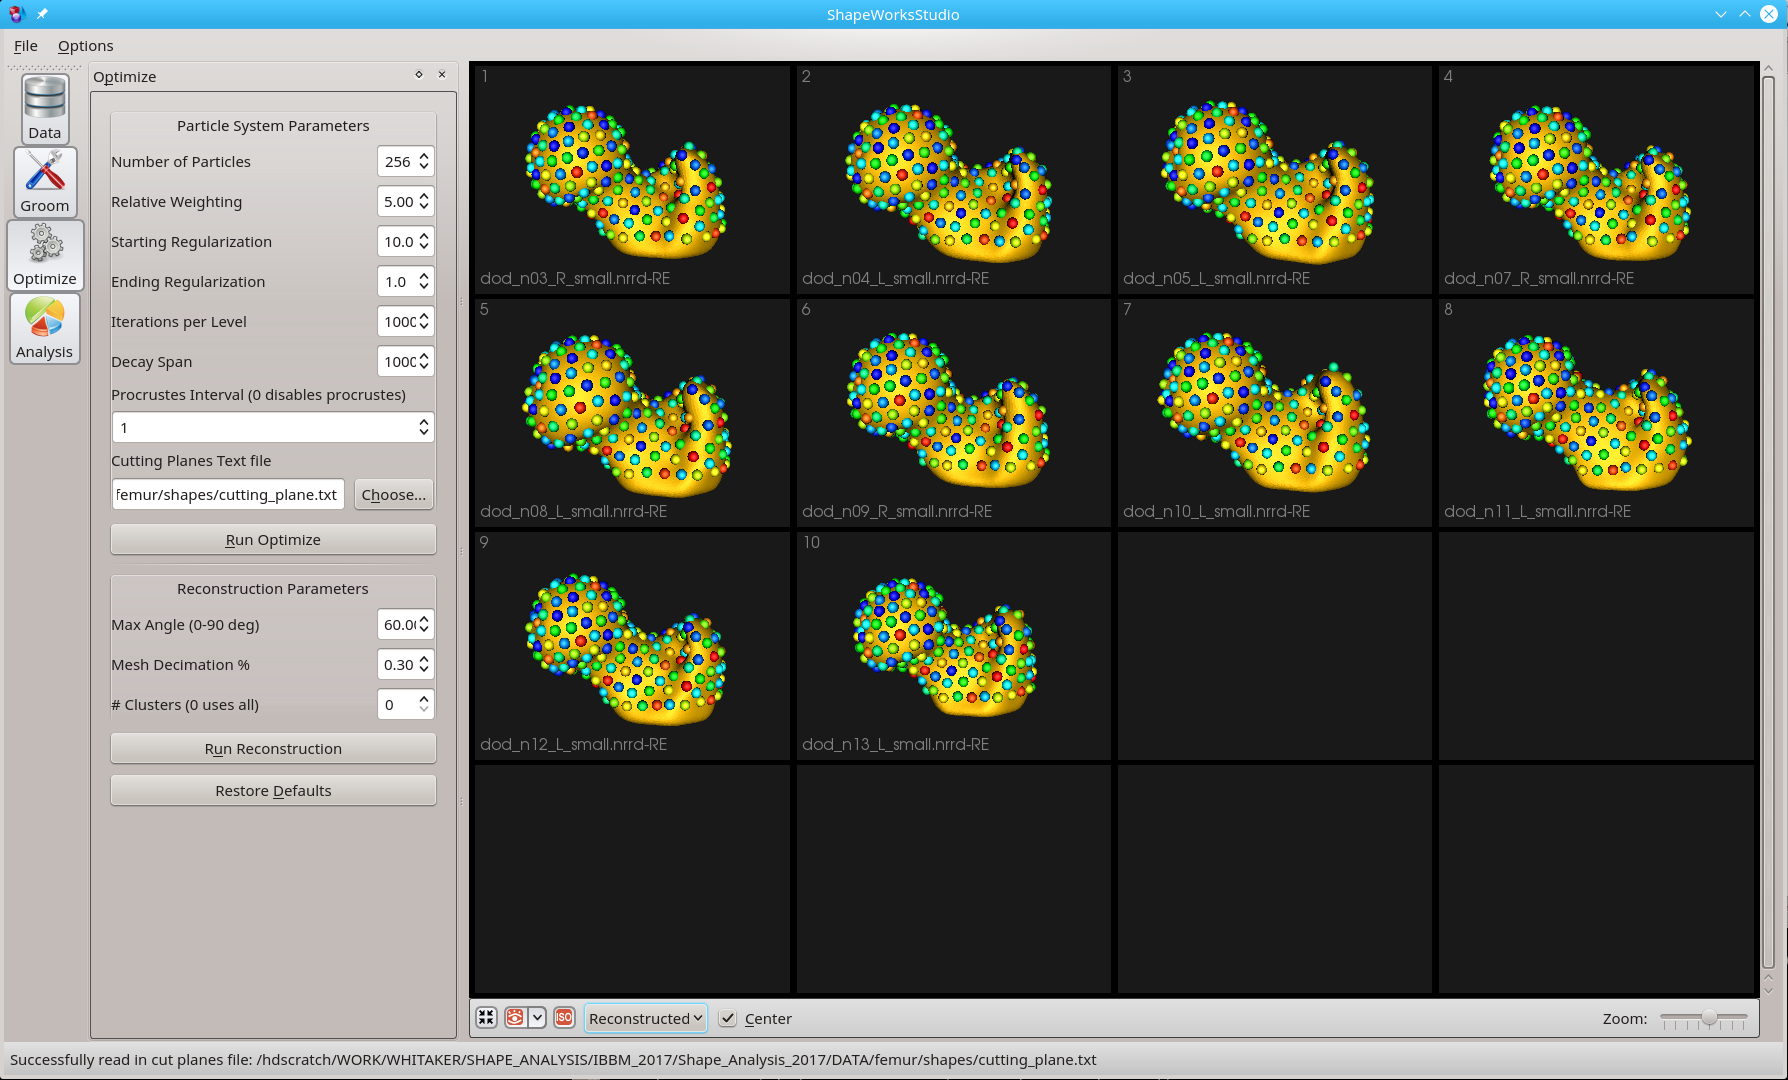
\includegraphics[width=0.9\textwidth]{figs_v2/femur_optimize_reconstructed.png}
	\caption{Optimized femur correspondence model using relative weighting $ = 5$ along with particle-based surface reconstruction.}
	\label{fig:femur_optimize_reconstructed}
\end{figure}

\begin{figure}[!htp]
	\centering
	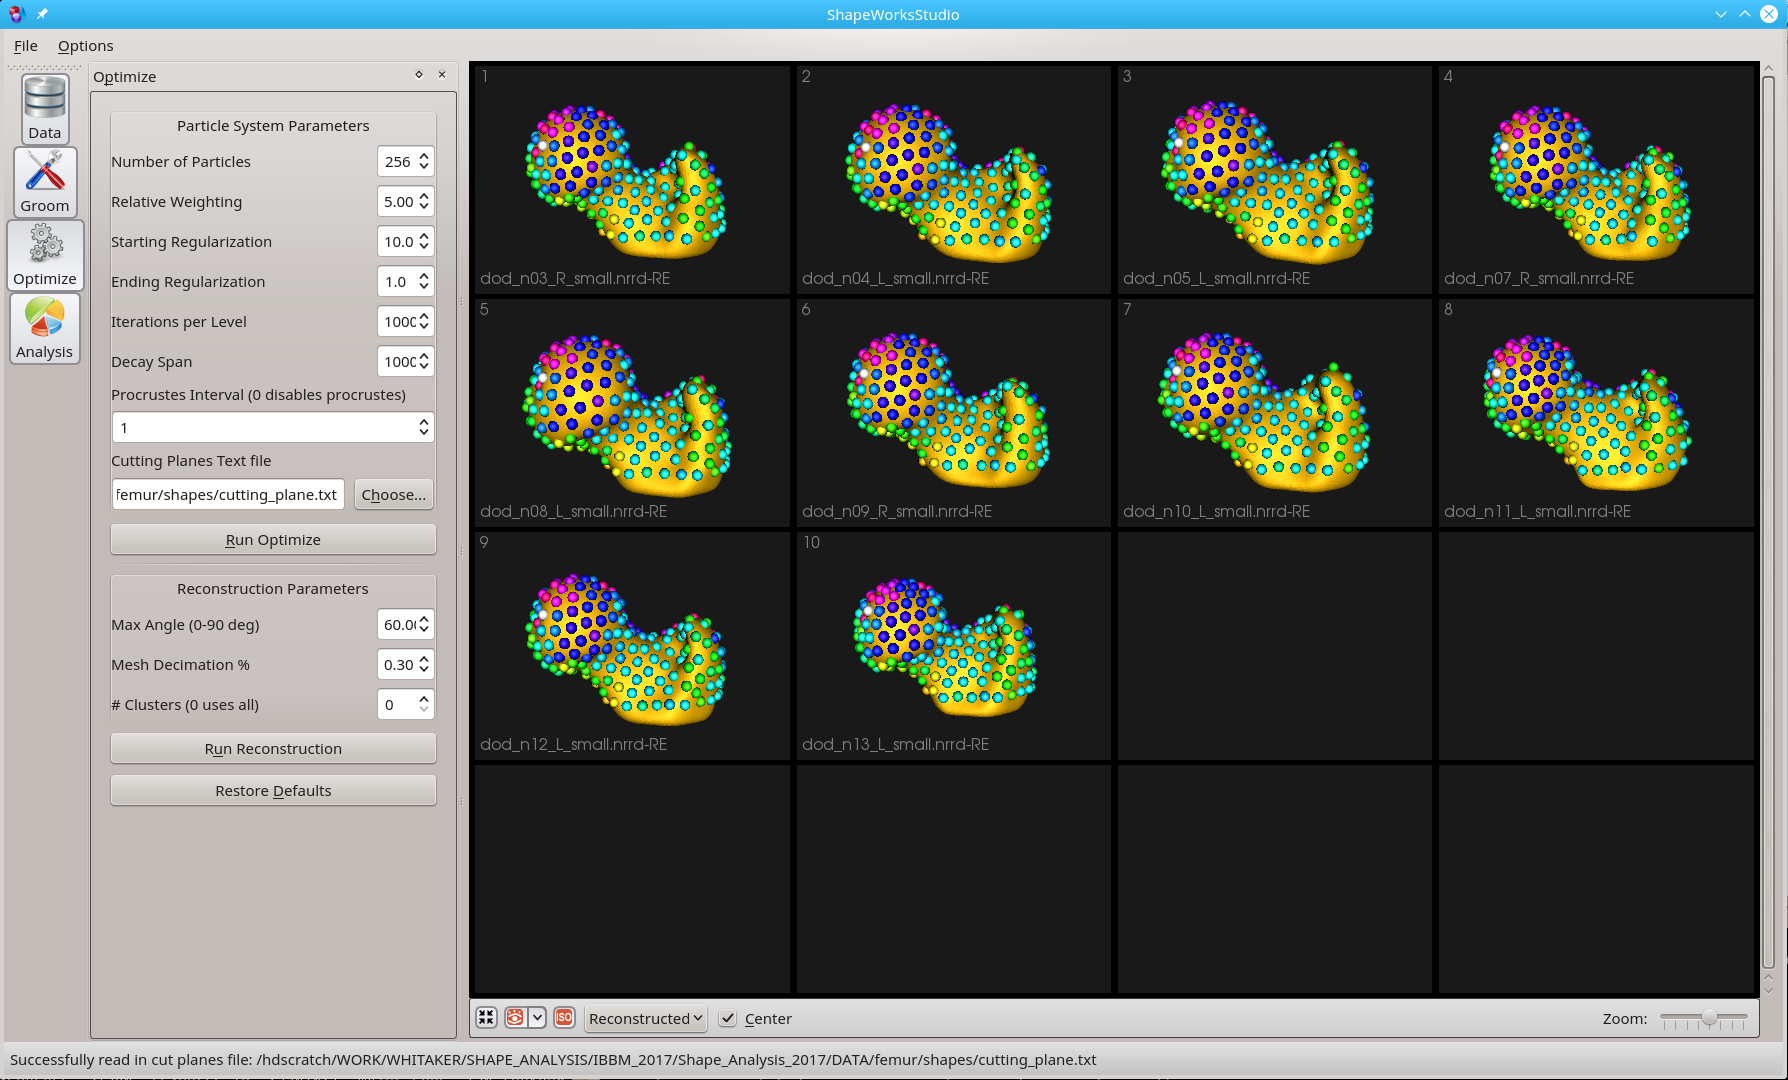
\includegraphics[width=0.83\textwidth]{figs_v2/femur_optimize_reconstructed_hover1.png}
	\caption{Optimized femur correspondence model using relative weighting $ = 5$ with one particle selected to visualize correspondence. Simply hover on the required particle and press 1, the particle will be colored in white and all other particles will be colored based on its distance to the selected particle. To recover the original display, type 1 or 2 while NOT hovering over any particles}
	\label{fig:femur_optimize_reconstructed_hover1}
\end{figure}

\begin{figure}[!htp]
	\centering
	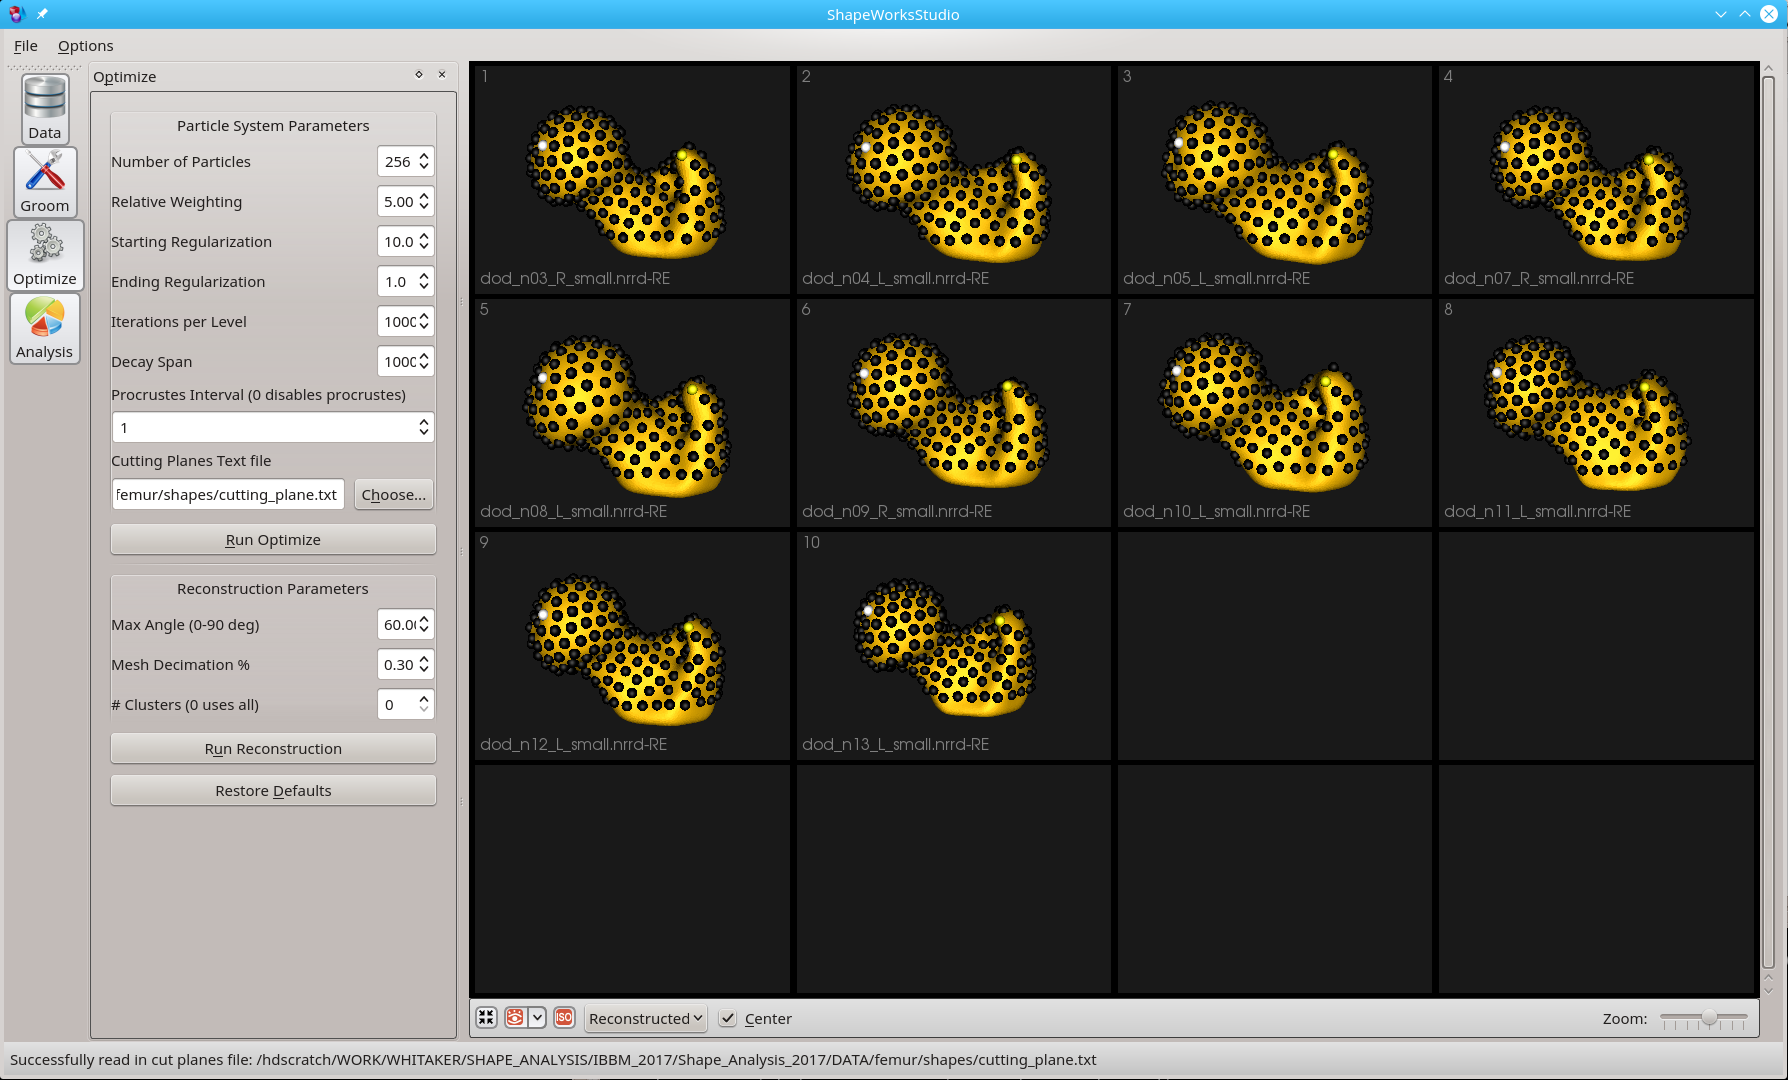
\includegraphics[width=0.83\textwidth]{figs_v2/femur_optimize_reconstructed_hover2.png}
	\caption{Optimized femur correspondence model using relative weighting $ = 5$ with two particles selected to visualize pairwise correspondence. Simply hover on the second required particle and press 2, the second particle will be colored in yellow and all other particles will be colored in black. To recover the original display, type 1 or 2 while NOT hovering over any particles}
	\label{fig:femur_optimize_reconstructed_hover2}
\end{figure}

\begin{figure}[!htp]
	\centering
	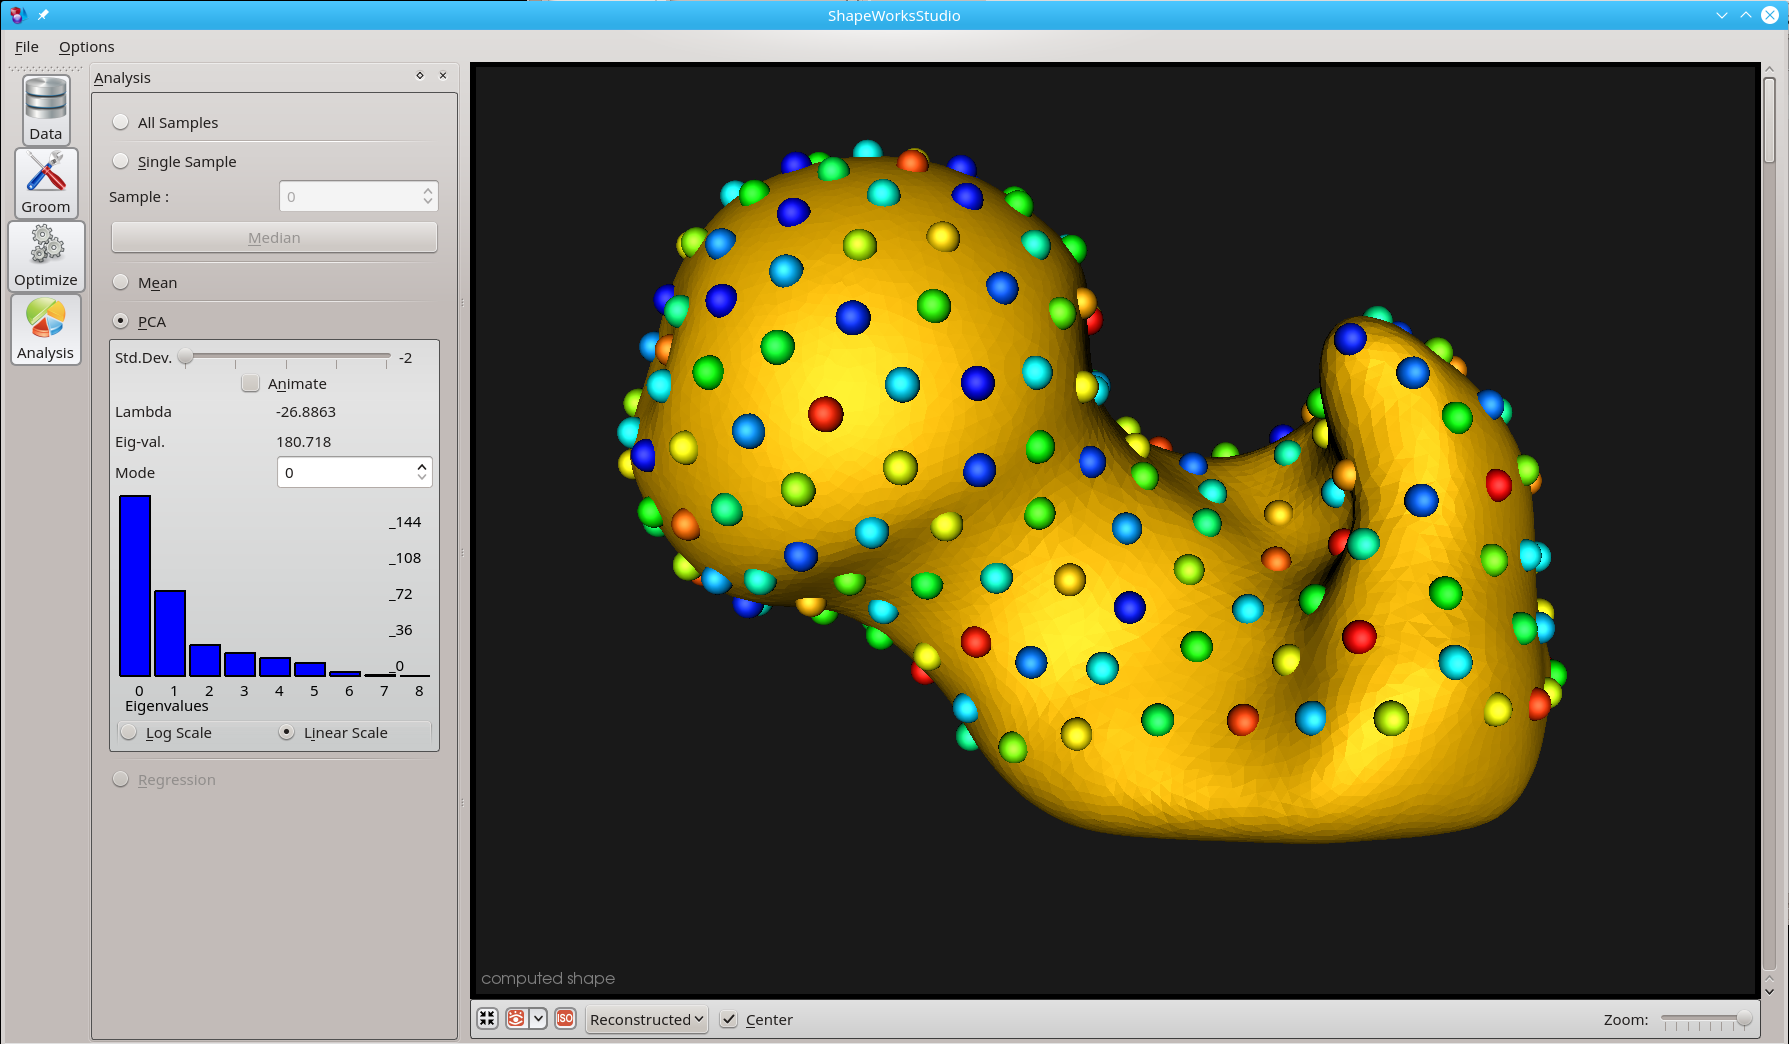
\includegraphics[width=0.32\textwidth]{figs_v2/femur_analyze_mode1_neg2std.png}
	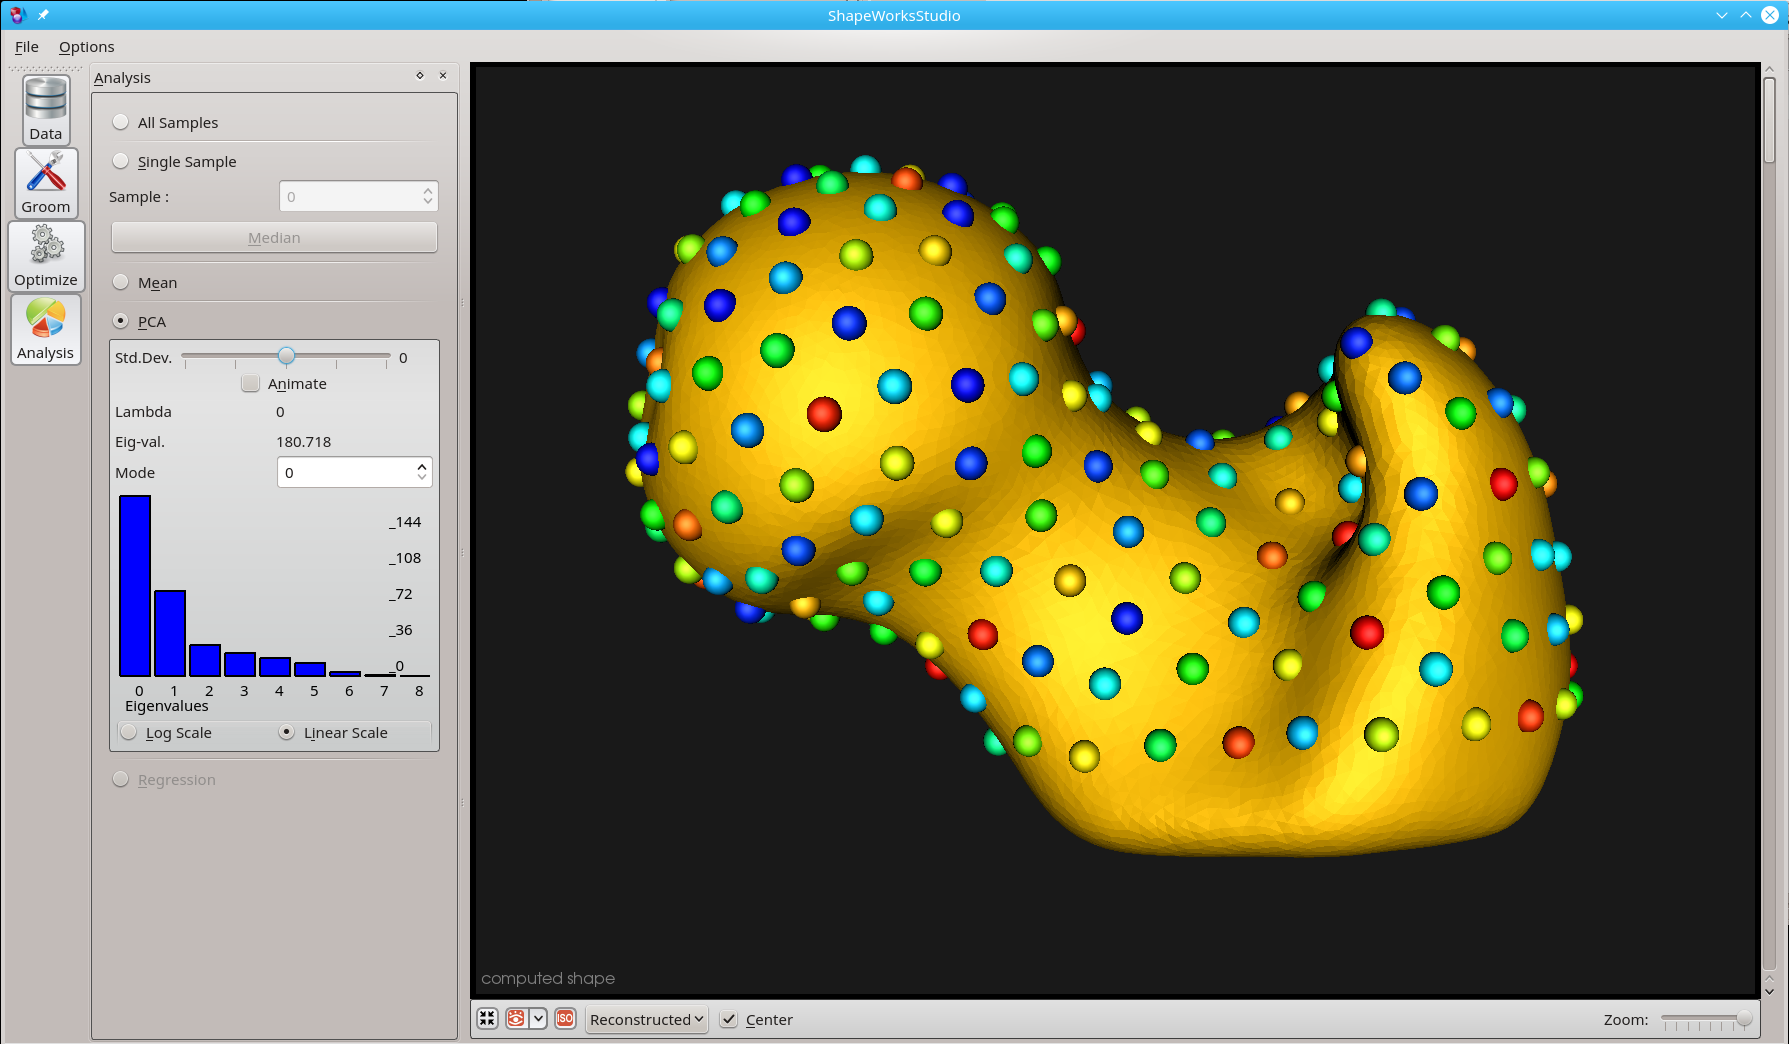
\includegraphics[width=0.32\textwidth]{figs_v2/femur_analyze_mode1_mean.png}
	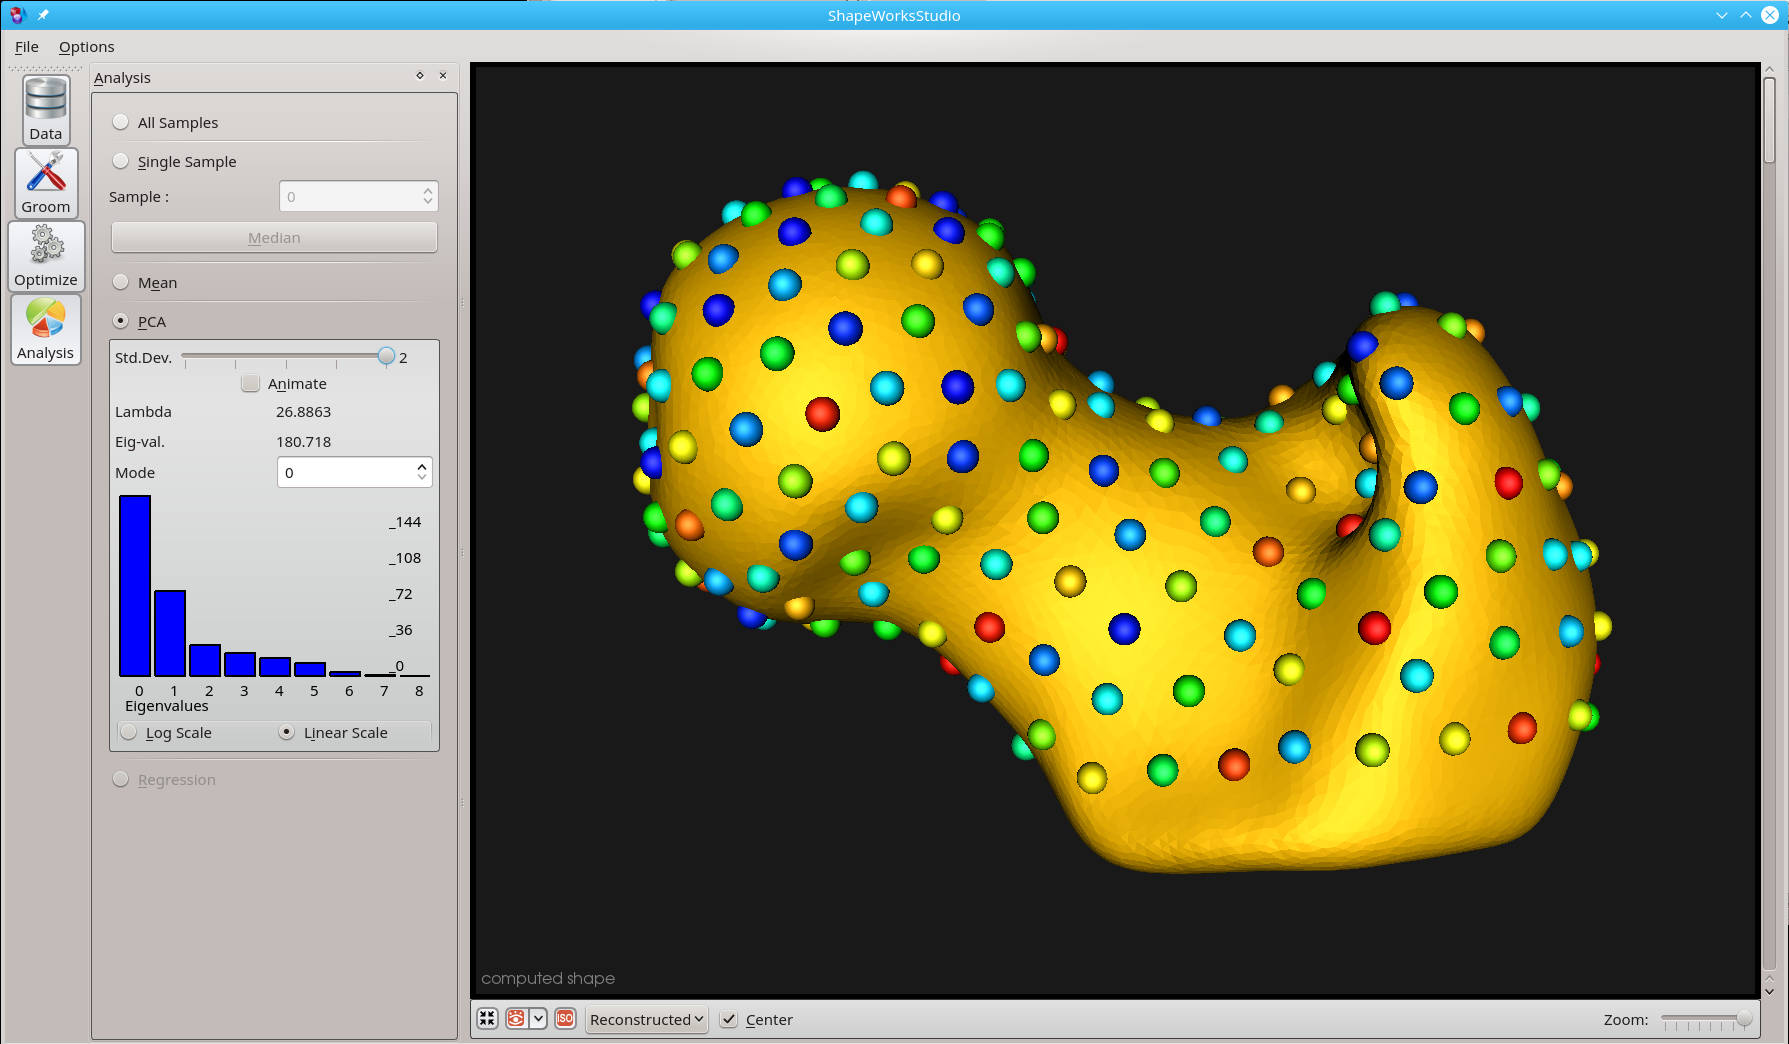
\includegraphics[width=0.32\textwidth]{figs_v2/femur_analyze_mode1_pos2std.png} \\
	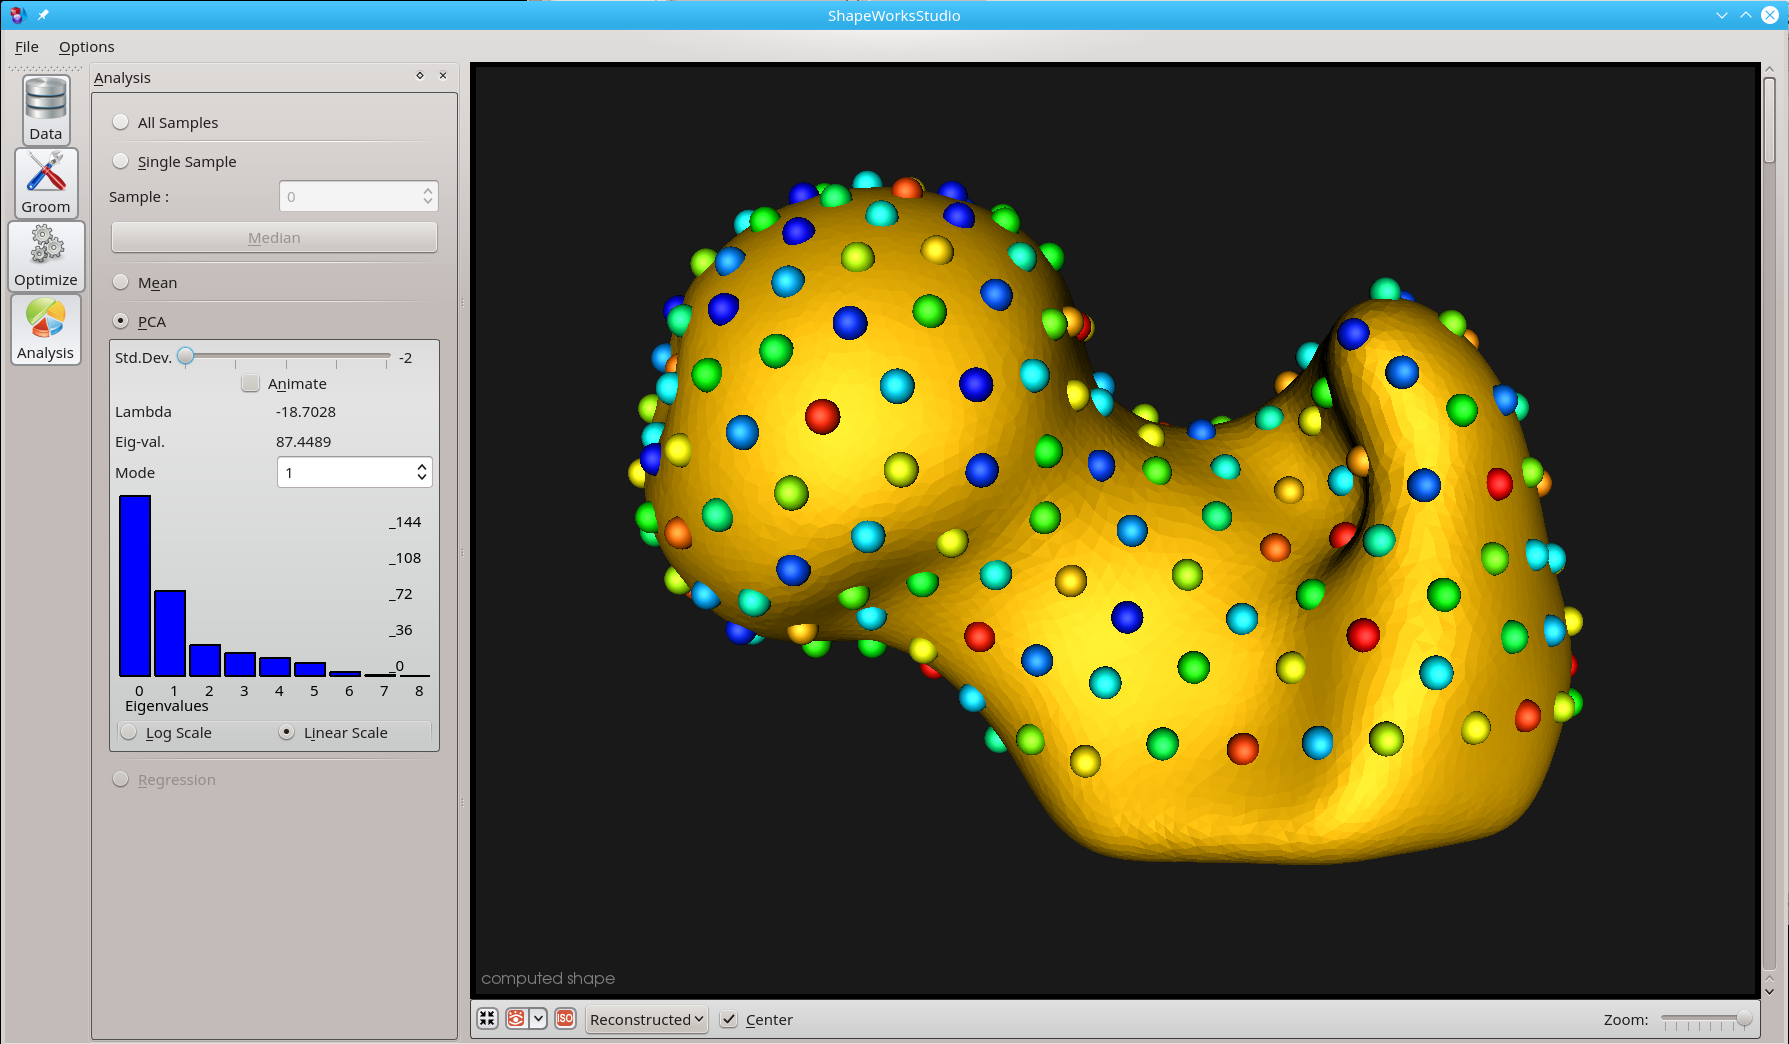
\includegraphics[width=0.32\textwidth]{figs_v2/femur_analyze_mode2_neg2std.png}
	\includegraphics[width=0.32\textwidth]{figs_v2/femur_analyze_mode1_mean.png}
	\includegraphics[width=0.32\textwidth]{figs_v2/femur_analyze_mode2_pos2std.png} \\
	\includegraphics[width=0.32\textwidth]{figs_v2/femur_analyze_mode3_neg2std.png}
	\includegraphics[width=0.32\textwidth]{figs_v2/femur_analyze_mode1_mean.png}
	\includegraphics[width=0.32\textwidth]{figs_v2/femur_analyze_mode3_pos2std.png} 	\\
	\includegraphics[width=0.32\textwidth]{figs_v2/femur_analyze_mode4_neg2std.png}
	\includegraphics[width=0.32\textwidth]{figs_v2/femur_analyze_mode4_mean.png}
	\includegraphics[width=0.32\textwidth]{figs_v2/femur_analyze_mode4_pos2std.png} 
	\caption{ Variations in PCA modes for the femur correspondence model (best seen using the animation option in studio). Top to bottom shows the first four dominant modes of the femur statistical model. Left to right shows variations in the PCA modes for -2 to 2 standard deviations. }
	\label{fig:femur_analyze_modes}
\end{figure}

\section{Important considerations and known issues}

\noindent\textbf{Image headers:} It is important that the image headers for your data contain correct and consistent image information. Pay special attention to the image spacing and origin information, as ShapeWorks software relies heavily on this information.

\vspace{0.1in}
\noindent\textbf{Setting parameters:} The authors highly recommend constructing a downsampled subset of your data to test parameter settings before running full optimizations. Create, for example, five or six test volumes that are no larger than $128^3$ pixels, so that a full initialization and optimization can be run in just a few minutes. 

\vspace{0.1in}
\noindent\textbf{Aliasing artifacts:} The authors highly recommend removing aliasing artifacts in your data, as they can adversly affect the quality of the correspondence optimization. You can use the Gaussian blurring included in the Studio release (Groom panel), however, if your shapes contains thin structures, you might want to consider other smoothing options that preserves the underlying topology.


\section{Contact, support and bug reports}

Please email any questions to \texttt{shapeworks-users@sci.utah.edu}. If there problems or bugs, please report them using the issue tracker on GitHub \texttt{https://github.com/SCIInstitute/ShapeWorksStudio/issues}. This includes feature requests. Feel free to add improvements using git pull requests. 

\bibliographystyle{osajnl} 
\bibliography{references.bib}
\end{document}
